% arara: xelatex: { shell: yes }
% arara: biber
% arara: xelatex: { shell: yes }
% arara: xelatex: { shell: yes }

%% This is the ctufit-thesis example file. It is used to produce theses
%% for submission to Czech Technical University, Faculty of Information Technology.
%%
%% Get the newest version from
%% https://gitlab.fit.cvut.cz/theses-templates/FITthesis-LaTeX
%%
%%
%% Copyright 2021, Eliska Sestakova and Ondrej Guth
%%
%% This work may be distributed and/or modified under the
%% conditions of the LaTeX Project Public Licenese, either version 1.3
%% of this license or (at your option) any later version.
%% The latest version of this license is in
%%  https://www.latex-project.org/lppl.txt
%% and version 1.3 or later is part of all distributions of LaTeX
%% version 2005/12/01 or later.
%%
%% This work has the LPPL maintenance status `maintained'.
%%
%% The current maintainer of this work is Ondrej Guth.
%% Contact ondrej.guth@fit.cvut.cz for bug reports.
%% Alternatively, submit bug reports into the tracker at
%% https://gitlab.fit.cvut.cz/theses-templates/FITthesis-LaTeX/issues
%%
%%

%%%%%%%%%%%%%%%%%%%%%%%%%%%%%%%%%%%%%%%%%
% CLASS OPTIONS
% language: czech/english/slovak
% thesis type: bachelor/master/dissertation
%%%%%%%%%%%%%%%%%%%%%%%%%%%%%%%%%%%%%%%%%
\documentclass[czech,bachelor,unicode]{template/ctufit-thesis}

%%%%%%%%%%%%%%%%%%%%%%%%%%%%%%%%%%
% FILL IN THIS INFORMATION
%%%%%%%%%%%%%%%%%%%%%%%%%%%%%%%%%%
\ctufittitle{Webová aplikace pro výuku programovacích jazyků} % replace with the title of your thesis
\ctufitauthorfull{Bc.\,Vojtěch Moravec} % replace with your full name (first name(s) and then family name(s) / surname(s)) including academic degrees
\ctufitauthorsurnames{Moravec} % replace with your surname(s) / family name(s)
\ctufitauthorgivennames{Vojtěch} % replace with your first name(s) / given name(s)
\ctufitsupervisor{Ing.\,Oldřich Malec} % replace with name of your supervisor/advisor (include academic degrees)
\ctufitdepartment{Katedra softwarového inženýrství} % replace with the department of your defence
\ctufityear{2024} % replace with the year of your defence
\ctufitdeclarationplace{Praze} % replace with the place where you sign the declaration
\ctufitdeclarationdate{\today} % replace with the date of signature of the declaration
\ctufitabstractCZE{%! Author = Vojta
%! Date = 25.11.2021

V této práci řeším, jak navrhnout a vytvořit prototyp webové aplikace, která má uživateli poskytnout jednotné rozhraní
pro vaření podle receptů, tedy správu receptů a surovin nebo například sdílení mezi uživateli.
Důraz je kladen na frontendovou část psanou ve Vue.js, ale popíšu i backend, který jsem tvořil pomocí platformy Firebase.
Nejdříve sesbírám požadavky od potencionálních uživatelů a zanalyzuji konkurenční řešení. Poté navrhnu design aplikace a
strukturu ukládání dat. Dále přiblížím technologie, které použiji k implementaci.
Na závěr aplikaci otestuji s pomocí respondentů, od kterých jsem získal požadavky, a doplním možná rozšíření do budoucna,
která by aplikaci učinila více komplexní a nabídla uživateli kompletní balíček bez potřeby použití dalších aplikací.
Výsledkem je veřejně přístupná aplikace, která pomůže každému, kdo hledá řešení pro ukládání receptů a dalších možností, které na nich staví.
}
\ctufitabstractENG{%! Author = Vojta
%! Date = 25.11.2021

This bachelor's thesis describes the design and implementation of a web application, which helps the user with using cooking recipes.
This is achieved by the management of recipes, ingredients, and sharing of those among the users. Emphasis is placed on the frontend part written in Vue.js.
I will also describe the backend, which was created using the development platform Firebase. I will start by collecting requirements from potential users
and by analyzing existing solutions. After that, I will create the design of the application and describe the structure of the data. Then I will introduce
the technologies used to implement the application. Finally, I will construct a user test and perform it with multiple respondents and describe possible extensions.
The result of this thesis is a web application, which is publicly accessible. It helps anyone who seeks a complete package for cooking recipes.
}
\ctufitkeywordsCZE{frontend, Vue, Vuetify, recepty na vaření, webová aplikace, serverless, Firebase} % TODO
\ctufitkeywordsENG{frontend, Vue, Vuetify, cooking recipes, web app, serverless, Firebase} % TODO
%%%%%%%%%%%%%%%%%%%%%%%%%%%%%%%%%%
% END FILL IN
%%%%%%%%%%%%%%%%%%%%%%%%%%%%%%%%%%

%%%%%%%%%%%%%%%%%%%%%%%%%%%%%%%%%%
% CUSTOMIZATION of this template
% Skip this part or alter it if you know what you are doing.
%%%%%%%%%%%%%%%%%%%%%%%%%%%%%%%%%%

\RequirePackage{iftex}[2020/03/06]
\iftutex % XeLaTeX and LuaLaTeX
    \RequirePackage{ellipsis}[2020/05/22] %ellipsis workaround for XeLaTeX
\else
    \RequirePackage[utf8]{inputenc}[2018/08/11] %this file encoding
    \RequirePackage{lmodern}[2009/10/30] % vector flavor of Computer Modern font
\fi

% hyperlinks
\RequirePackage[pdfpagelayout=TwoPageRight,colorlinks=false,allcolors=decoration,pdfborder={0 0 0.1}]{hyperref}[2020-05-15]

% uncomment the following to hide all hyperlinks
% \RequirePackage[pdfpagelayout=TwoPageRight,hidelinks]{hyperref}[2020-05-15]

\RequirePackage{pdfpages}[2020/01/28]

\setcounter{secnumdepth}{4} % numbering sections; 4: subsubsection



%%%%%%%%%%%%%%%%%%%%%%%%%%%%%%%%%%
% CUSTOMIZATION of this template END
%%%%%%%%%%%%%%%%%%%%%%%%%%%%%%%%%%


%%%%%%%%%%%%%%%%%%%%%%
% DEMO CONTENTS SETTINGS
% You may choose to modify this part.
%%%%%%%%%%%%%%%%%%%%%%
\usepackage{dirtree}
\usepackage{lipsum,tikz}
\usepackage{csquotes}
\addbibresource{text/bib-database.bib}
%\usepackage{listings} % typesetting of sources
\usepackage{minted}
\usepackage{graphicx} % typesetting of sources
\usepackage[allfiguresdraft]{draftfigure} % TODO: Comment this line to get images rendered
\usepackage{subfig}
\usepackage{tabularx}
\usepackage{xevlna}		% for non-breakable whitespaces

\renewcommand\theFancyVerbLine{\normalsize\arabic{FancyVerbLine}}

% Custom colors
\definecolor{recipeo-light-green}{RGB}{121, 255, 161}
\definecolor{recipeo-light-blue}{RGB}{29, 125, 238}
\definecolor{recipeo-dark-green}{HTML}{4CA262}
\definecolor{recipeo-dark-blue}{HTML}{4372B4}

%theorems, definitions, etc.
\theoremstyle{plain}
\newtheorem{theorem}{Věta}
\newtheorem{lemma}[theorem]{Tvrzení}
\newtheorem{corollary}[theorem]{Důsledek}
\newtheorem{proposition}[theorem]{Návrh}
\newtheorem{definition}[theorem]{Definice}
\theoremstyle{definition}
\newtheorem{example}[theorem]{Příklad}
\theoremstyle{remark}
\newtheorem{note}[theorem]{Poznámka}
\newtheorem*{note*}{Poznámka}
\newtheorem{remark}[theorem]{Pozorování}
\newtheorem*{remark*}{Pozorování}
\numberwithin{theorem}{chapter}
%theorems, definitions, etc. END
%%%%%%%%%%%%%%%%%%%%%%
% DEMO CONTENTS SETTINGS END
%%%%%%%%%%%%%%%%%%%%%%

\begin{document}
\frontmatter\frontmatterinit % do not remove these two commands

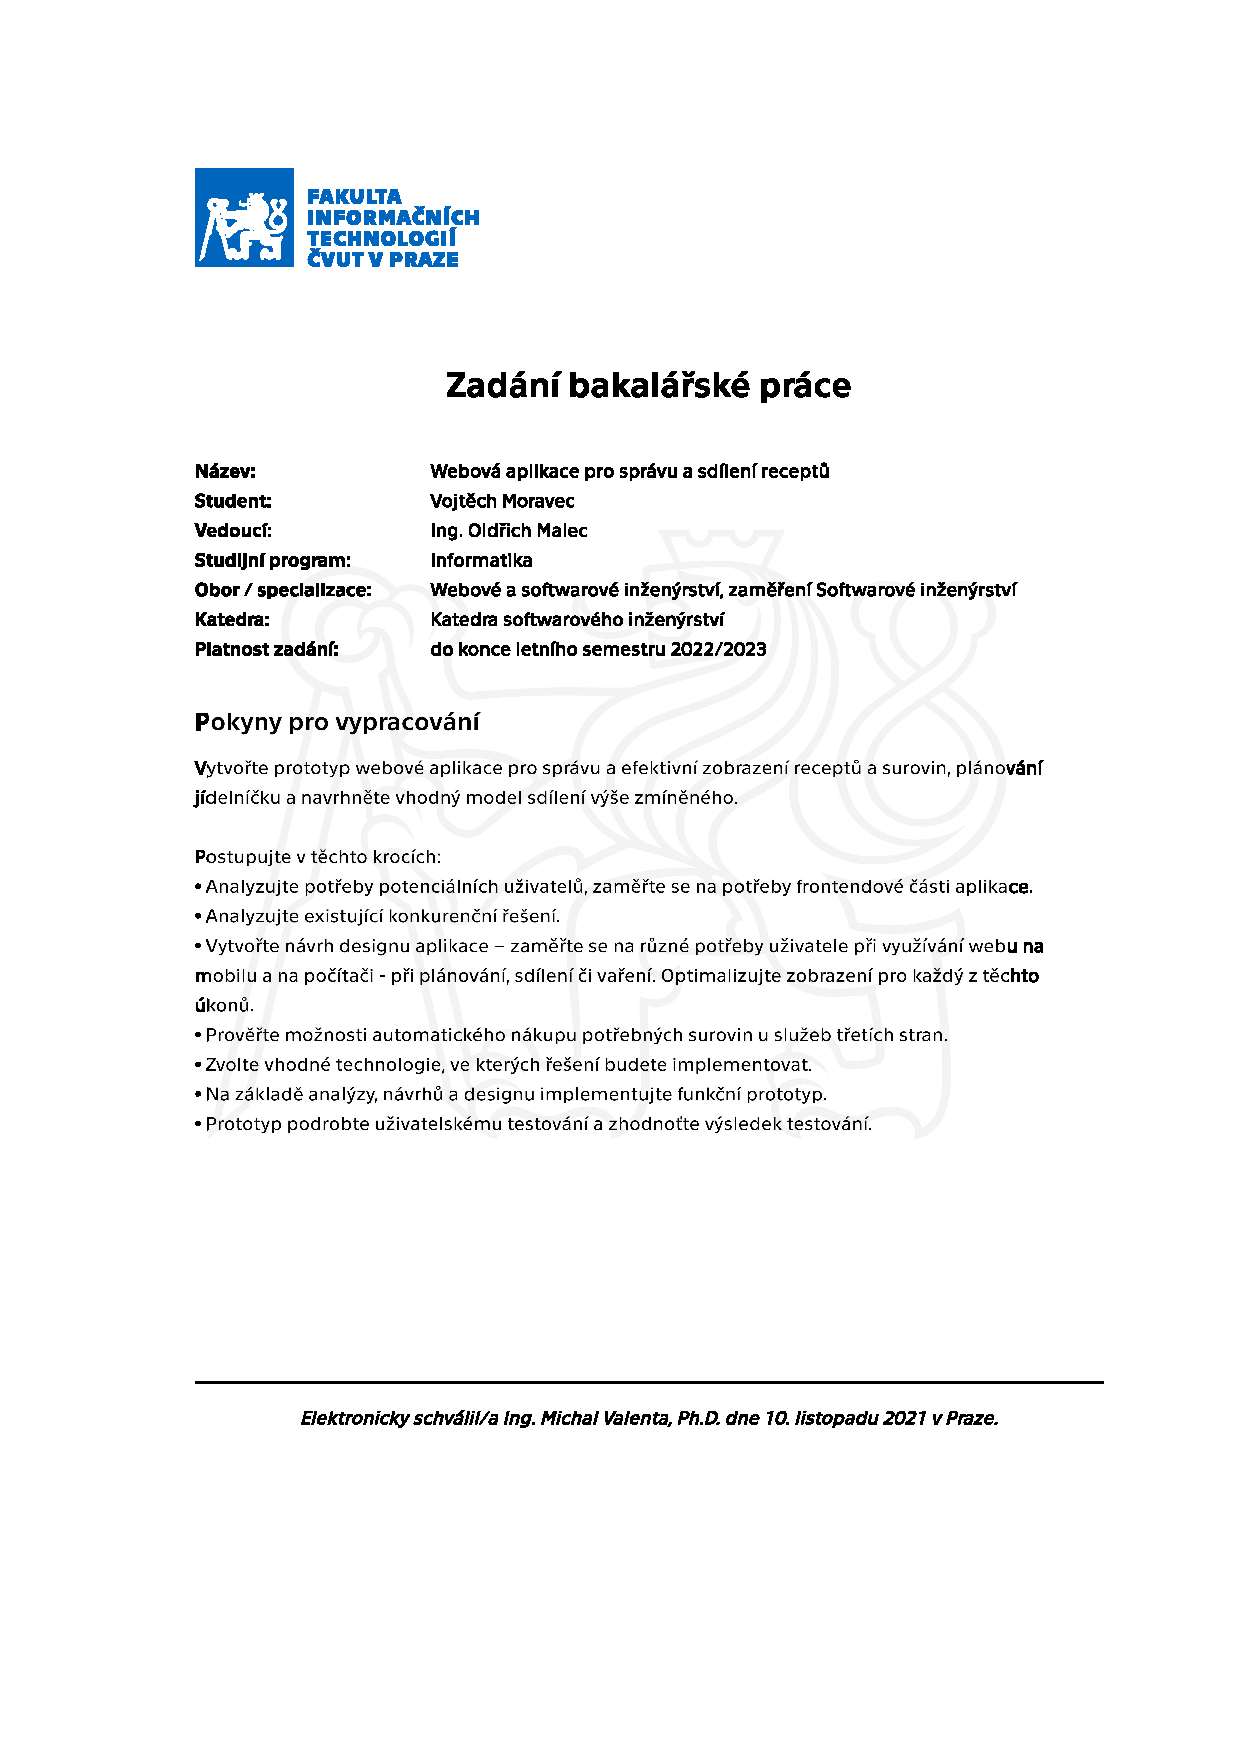
\includepdf{pdf/assignment-include.pdf} % replace that file with your thesis assignment provided by study office

\thispagestyle{empty}\cleardoublepage\maketitle % do not remove these three commands

\imprintpage % do not remove this command

\tableofcontents % do not remove this command
%%%%%%%%%%%%%%%%%%%%%%
% list of other contents: figures, tables, code listings, algorithms, etc.
% add/remove commands accordingly
%%%%%%%%%%%%%%%%%%%%%%
\listoffigures % list of figures
\begingroup
\let\clearpage\relax
\listoftables % list of tables
%\lstlistoflistings % list of source code listings generated by the listings package TODO: Minted switch
\listoflistings % list of source code listings generated by the minted package
\endgroup
%%%%%%%%%%%%%%%%%%%%%%
% list of other contents END
%%%%%%%%%%%%%%%%%%%%%%

%%%%%%%%%%%%%%%%%%%
% ACKNOWLEDGMENT
% FILL IN / MODIFY
% This is a place to thank people for helping you. It is common to thank your supervisor.
%%%%%%%%%%%%%%%%%%%
\begin{acknowledgmentpage}
	Chtěl bych poděkovat především vedoucímu této práce Ing.~Oldřichu~Malcovi za odborné vedení mé práce, za jeho čas a cenné rady.
    Dále bych chtěl poděkovat všem respondentům, kteří mi pomohli získat přehled o potřebách uživatelů. V neposlední řadě patří obrovské
    poděkování mé rodině, díky které jsem mohl studovat bez jakýchkoliv problémů.
\end{acknowledgmentpage}
%%%%%%%%%%%%%%%%%%%
% ACKNOWLEDGMENT END
%%%%%%%%%%%%%%%%%%%


%%%%%%%%%%%%%%%%%%%
% DECLARATION
% FILL IN / MODIFY
%%%%%%%%%%%%%%%%%%%
% INSTRUCTIONS
% ENG: choose one of approved texts of the declaration. DO NOT CREATE YOUR OWN. Find the approved texts at https://courses.fit.cvut.cz/SFE/download/index.html#_documents (document Declaration for FT in English)
% CZE/SLO: Vyberte jedno z fakultou schvalenych prohlaseni. NEVKLADEJTE VLASTNI TEXT. Schvalena prohlaseni najdete zde: https://courses.fit.cvut.cz/SZZ/dokumenty/index.html#_dokumenty (prohlášení do ZP)
\begin{declarationpage}
    Prohlašuji, že jsem předloženou práci vypracoval samostatně a že jsem uvedl veškeré
    použité informační zdroje v souladu s Metodickým pokynem o dodržování etických
    principů při přípravě vysokoškolských závěrečných prací.

    Beru na vědomí, že se na moji práci vztahují práva a povinnosti vyplývající ze zákona
    č. 121/2000 Sb., autorského zákona, ve znění pozdějších předpisů. V souladu s ust.
    § 2373 odst. 2 zákona č. 89/2012 Sb., občanský zákoník, ve znění pozdějších předpisů,
    tímto uděluji nevýhradní oprávnění (licenci) k užití této mojí práce, a to včetně všech
    počítačových programů, jež jsou její součástí či přílohou a veškeré jejich
    dokumentace (dále souhrnně jen „Dílo“), a to všem osobám, které si přejí Dílo užít.
    Tyto osoby jsou oprávněny Dílo užít jakýmkoli způsobem, který nesnižuje hodnotu
    Díla, avšak pouze k nevýdělečným účelům. Toto oprávnění je časově, teritoriálně
    i množstevně neomezené.
\end{declarationpage}
%%%%%%%%%%%%%%%%%%%
% DECLARATION END
%%%%%%%%%%%%%%%%%%%

\printabstractpage % do not remove this command

%%%%%%%%%%%%%%%%%%%
% SUMMARY
% FILL IN / MODIFY
% OR REMOVE ENTIRELY (upon agreement with your supervisor)
% (appropriate to remove in most theses)
%%%%%%%%%%%%%%%%%%%
%\begin{summarypage}
%\section*{Summary section}
%
%\lipsum[1][1-8]
%
%\section*{Summary section}
%
%\lipsum[2][1-6]
%
%\section*{Summary section}
%
%\lipsum[3]
%
%\section*{Summary section}
%
%\lipsum[2]
%
%\section*{Summary section}
%
%\lipsum[1][1-8] Lorem lorem lorem.
%\end{summarypage}
%%%%%%%%%%%%%%%%%%%
% SUMMARY END
%%%%%%%%%%%%%%%%%%%

%%%%%%%%%%%%%%%%%%%
% ABBREVIATIONS
% FILL IN / MODIFY
% OR REMOVE ENTIRELY
% List the abbreviations in lexicography order.
%%%%%%%%%%%%%%%%%%%
%! Author = vojmo
%! Date = 15.11.2021

\chapter{Seznam zkratek}

\begin{tabular}{rl}
    CLI     & Command Line Interface \\
    CSS     & Cascading Style Sheets \\
    FE      & Frontend \\
    IT      & Informační technologie \\
    JS      & JavaScript \\
    JSON    & JavaScript Object Notation \\
    NPM     & Node Package Manager \\
    PC      & Personal Computer \\
    SPA     & Single Page Application \\
    SSR     & Server Side Rendering \\
    UI      & User interface \\
    URL     & Uniform Resource Locator \\
\end{tabular}

%! Author = Vojta
%! Date = 21.1.2024

\chapter{Slovník}

\begin{tabular}{rp{0.7\textwidth}}
    Accordion           & Rozbalovací menu \tabularnewline
    Auth                & Autentizace \tabularnewline
    Auto-scroll         & Automatické posouvání \tabularnewline
    Badge               & Odznak \tabularnewline
    Build               & Sestavení aplikace do finální podoby \tabularnewline
    Button              & Tlačítko \tabularnewline
    Card                & Karta \tabularnewline
    Carousel            & Posuvný prvek \tabularnewline
    Components          & Komponenty \tabularnewline
    Composable          & Znovupoužitelná funkce zachovávající stav \tabularnewline
    Contact             & Kontakt \tabularnewline
    Container           & Kontejner \tabularnewline
    Checkbox            & Zaškrtávací políčko \tabularnewline
    Dashboard           & Stránka s přehledem \tabularnewline
    Deploy              & Nasazení aplikace do testovacího či prostředí \tabularnewline
    Dropdown            & Rozbalovací menu \tabularnewline
    Endpoint            & Bod API, který obsahuje logiku a odpovídá daty \tabularnewline
    Error               & Chyba \tabularnewline
    Features            & Funkce \tabularnewline
    Flexbox             & CSS technologie pro uspořádání prvků na stránce \tabularnewline
    Fork                & Vytvoření kopie repozitáře \tabularnewline
    Framework           & Softwarové řešení pro podporu programování, vývoje a organizaci jiných softwarových projektů \tabularnewline
    Frontend            & Část aplikace, kterou vidí uživatel a reaguje s ní \tabularnewline
    Getting started     & První kroky \tabularnewline
    Headless            & Aplikace, která nemá vlastní frontend a komunikuje pouze přes API \tabularnewline
    Header              & Hlavička \tabularnewline
    Hero sekce          & Úvodní sekce \tabularnewline
    Highlighter         & Zvýrazňovač \tabularnewline
    Hook                & Volání funkce \tabularnewline
    Hosting             & Služba hostování webové stránky \tabularnewline
    Hot reload          & Automatické načítání změn \tabularnewline
    Hover               & Najetí myši na prvek \tabularnewline
    Icon                & Ikona \tabularnewline
    Inject              & Vložit \tabularnewline
    Issues              & Problémy v repozitáři \tabularnewline
    Loading             & Načítání \tabularnewline
    Landing page        & Úvodní stránka \tabularnewline
    Layout              & Rozložení stránky \tabularnewline
    Metaframework       & Framework postavený nad jiným frameworkem \tabularnewline
    Notification        & Oznámení \tabularnewline
    Open source         & Otevřený zdrojový kód (kdokoliv k němu může přistoupit a zároveň do něj přispět) \tabularnewline
    Pagination          & Stránkování \tabularnewline
    Patch               & Oprava chyby \tabularnewline
    Pattern matching    & Porovnávání vzorů \tabularnewline
    Pop-up              & Vyskakovací okno \tabularnewline
    Popover             & Plovoucí okno \tabularnewline
    Pull request        & Žádost o změnu ve zdrojovém kódu \tabularnewline
    Push                & Nahrání změněného kódu do repozitáře \tabularnewline
\end{tabular}

\begin{tabular}{rp{0.7\textwidth}}
    Prop                & Vlastnost komponenty \tabularnewline
    Props               & Vlastnosti komponenty \tabularnewline
    Provide            & Poskytovat \tabularnewline
    References          & Reference \tabularnewline
    Section             & Sekce \tabularnewline
    Select              & Prvek pro výběr \tabularnewline
    Sidebar             & Postranní panel \tabularnewline
    Slot                & Místo pro vložení obsahu \tabularnewline
    Slots               & Místa pro vložení obsahu \tabularnewline
    Switch              & Přepínač \tabularnewline
    Table               & Tabulka \tabularnewline
    Tabs                & Karty \tabularnewline
    Textarea            & Víceřádkové textové pole \tabularnewline
    Text input          & Jednořádkové textové pole \tabularnewline
    Tooltip             & Pomocný text při najetí myši na prvek \tabularnewline
    Tree shaking        & Odstranění nepoužitých částí kódu \tabularnewline
    Utility-first       & Přístup k tvorbě stylů, kde se využívají jednoduché a malé třídy (tedy dává přednost funkčnosti) \tabularnewline
    Wireframe           & Drátěný model \tabularnewline
    Wrapper             & Obal \tabularnewline
\end{tabular}


% This part is to get rid of the `Kapitola 0` text on empty page
\makeatletter
\def\cleardoublepagecustom{\clearpage\if@twoside \ifodd\c@page\else
\hbox{}\thispagestyle{empty}\newpage\if@twocolumn\hbox{}\newpage\fi\fi\fi}
\makeatother

\cleardoublepagecustom
%%%%%%%%%%%%%%%%%%%
% ABBREVIATIONS END
%%%%%%%%%%%%%%%%%%%

\mainmatter\mainmatterinit % do not remove these two commands

%%%%%%%%%%%%%%%%%%%
% THE THESIS
% MODIFY ANYTHING BELOW THIS LINE
%%%%%%%%%%%%%%%%%%%

%! Author = Vojta
%! Date = 21.1.2024

\chapter{Úvod}
V moderním světě vývoje webových aplikací se neustále zvyšuje důraz na efektivitu, opakovanou použitelnost a rychlost implementace. Tyto vlastnosti jsou důležité zejména v kontextu stále rostoucích požadavků na kvalitu uživatelských rozhraní (UI) a uživatelského zážitku (UX). Vývojáři se proto stále častěji obracejí k využití UI knihoven, které jim poskytují předdefinované komponenty a nástroje pro rychlé a efektivní vytváření komplexních a esteticky příjemných rozhraní. Tyto knihovny jsou důležitou součástí vývoje aplikací, protože usnadňují implementaci složitých UI prvků.

Nicméně jeden z problému dnešních knihoven je ten, že vývojáři nemohou jednoduše modifikovat nebo rozšiřovat existující komponenty. To může vést k problémům při vytváření unikátních a přizpůsobených uživatelských rozhraní.

Tato práce se zabývá analýzou různých aspektů UI knihoven, včetně jejich designu, funkcí. Cílem je poskytnout ucelený pohled na UI knihovny, jejich výhody, výzvy a \emph{best practices} pro jejich využití ve webovém vývoji.


\chapter{Cíl}
Hlavním cílem této práce je vytvořit sbírku znovupoužitelných a snadno modifikovatelných komponent pro webové aplikace postavené na \emph{frameworku} Nuxt. Tato sbírka komponent má usnadnit počáteční fázi vývoje, nabídnout možnosti rozšíření a přizpůsobení podle individuálních potřeb. Práce se nezaměřuje pouze na vývoj samotných komponent, ale zahrnuje také jejich podrobnou dokumentaci a nástroje, které podporují všechny fáze tvoření aplikace – od návrhu až po nasazení.

V teoretické části práce je popsán výběr zvolených technologií a analýza existujících řešení, která mohou sloužit jako inspirace pro tvorbu komponent. Tato analýza zahrnuje detailní přehled různých přístupů k vývoji UI knihoven, jejich výhod a nevýhod, a posouzení, jak tyto přístupy ovlivňují efektivitu a flexibilitu vývoje. Důkladně jsou prozkoumány existující knihovny komponent, jako jsou například Nuxt UI a Radix UI, a jejich přínosy a omezení v kontextu konkrétních projektů. Rovněž jsou porovnány dva hlavní přístupy k integraci komponent do projektů – distribuce pomocí balíčků versus vlastnění kódu.

Praktická část se věnuje návrhu, vývoji a testování sbírky, dokumentace a možnostem budoucího rozšíření. Proces návrhu zahrnuje tvorbu návrhů jednotlivých komponent. Vývoj komponent je prováděn s důrazem na dodržování \emph{best practices} a použití moderních nástrojů a technologií, jako jsou Vue, Nuxt, TypeScript a Tailwind CSS. V této části jsou rovněž popsány konkrétní techniky používané při implementaci. Testování zahrnuje uživatelské testování, aby bylo zajištěno, že komponenty splňují stanovené požadavky a jsou snadno použitelné.

%! Author = Vojta
%! Date = 21.1.2024

\chapter{Analýza}

\section{Kvalitativní průzkum}
Vzhledem k tomu, že se jedná o projekt, který je určený hlavně pro využití autora, není kvalitatní průzkum příliš relevantní.
Místo toho se práce zaměřuje na porovnání existujících řešení, jejich výhod a nevýhod a názorů komunity.
Nicméně v jedné z následujících kapitol jsou výsledky z testování a výčet následných úprav.

\section{Existující řešení}

Existující řešení lze rozdělit do dvou skupin. První skupinou jsou knihovny, které nabízejí sadu komponent jako balíček, který
se do projektu přidá jako závislost. Poté se komponenty importují a používají v kódu. Jejich stylování lze upravit, ale většinou
pouze pomocí předpřipravených proměnných nebo limitovaným rozhraním. Úprava jejich funkcionality je většinou velmi omezená. Jakmile
chce uživatel upravit větší části, musí přistoupit k ohybání kódu, což často vede k neudržitelnému kódu.

Druhou skupinou jsou knihovny, které nejsou připraveny pro použití jako balíček. Jejich kód je dostupný pro zkopírování do projektu,
popř. mají dostupné CLI, které umožňuje komponenty přidat pomocí jednoduchého příkazu. Tato skupina míří na lepší znovupoužitelnost kódu
a zároveň na vyšší možnosti rozšíření a úprav.

\clearpage

\subsection{Knihovny s principem balíčkování}

\subsubsection{NuxtUI}
Jako zástupce knihoven na principu balíčkování jsem si vybral NuxtUI. Tuto knihovnu jsem využil na několika projektech, takže jsem si
dokázal udělat představu o jejích výhodách a nevýhodách. Líbilo se mi, že nabízí velké množství komponent, které jsou propracované a hezky
nastylované. Na druhou stranu jsem se často potýkal s tím, že jsem chtěl upravit funkčnost komponenty, ale nebylo to možné. Většinou jsem
musel přistoupit k vytvoření ohnutí ruzných částí. Tyto úpravy byly často velmi složité a neudržitelné.

\begin{itemize}
    \item \textbf{Výhody}
    \begin{itemize}
        \item Velké množství komponent
        \item Propracované styly
        \item Připravené pro použití
    \end{itemize}
    \item \textbf{Nevýhody}
    \begin{itemize}
        \item Omezené možnosti úprav
        \item Složité úpravy stylů

        \item Složité úpravy funkcionality
    \end{itemize}
\end{itemize}

\subsection{Knihovny s principem vlastnění kódu}
Knihovny, kde výsledný kód vlastníte většinou obsahují komponenty, které jsou jednodušší. Jejich výhodou je, že je lze snadno upravit, protože
kód není schovaný v balíčku. Nevýhodou je, že některé složitejší operace si uživatel musí vytvořit sám. Je tu ale jedna vyjímka, na kterou se chci
zaměřit, protože na podobném principu chci stavět i svojí kolekci.

% https://www.radix-ui.com/primitives/docs/overview/introduction
\subsubsection{Radix UI}
RadixUI představuje open-source knihovnu UI komponent, která je zaměřena na tvorbu kvalitních a přístupných designových systémů a webových aplikací.
Jde především o Radix Primitives, což jsou nízkoúrovňové UI komponenty s důrazem na přístupnost a možnost úprav vývojářů za cílem vytvoření vlastní knihovny.
Tyto komponenty lze využívat buď jako základní vrstvu designového systému nebo je postupně implementovat do stávajících projektů. \cite{RadixUIPrimitives}

\subsubsection{shadcn/ui}
Shadcn/ui je inovativní open-source knihovna UI komponent, která je navržena tak, aby vylepšila webový vývoj, zejména pro projekty využívající React.
Hlavní předností této knihovny je její lehkost, díky čemuž se snadno integruje do projektů bez nutnosti zatěžujících závislostí. Knihovna staví
zejména na komponentách Radix UI, které kladou důrat na přístupnost, což zajišťuje, že komponenty jsou inkluzivní a použitelné pro všechny uživatele. \cite{ShadcnUI}

Dalším významným aspektem knihovny Shadcn/ui je integrace s frameworkem Tailwind CSS, který poskytuje efektivní a přívětivé prostředí pro vývojáře,
preferující tento CSS framework orientovaný na utilitu. Výhody Tailwind CSS jsou popsány v kapitole věnované technologiím. Tato integrace umožňuje snadnou úpravu
a rozšíření stylů. Shadcn/ui vyniká svou snadnou použitelností a detailní kontrolou nad komponentami. Vývojáři mohou přímo přistupovat ke zdrojovému kódu
jednotlivých komponent, což umožňuje jejich efektivní úpravy pro specifické případy užití a požadavky aplikace.

Ruční instalace nebo kopírování každé komponenty může být pro některé vývojáře zdlouhavé, zejména pro ty, kteří jsou zvyklí importovat komponenty z balíčků.
Ačkoli přímý přístup ke kódu komponent prospívá modularitě a rozšiřitelnosti, může vést k rozšíření objemu kódu.

% Headless UI

\begin{itemize}
    \item \textbf{Výhody}
    \begin{itemize}
        \item Jednoduché úpravy
        \item Kód vlastní uživatel
        \item Aktualizace knihovny neovlivní kód
    \end{itemize}
    \item \textbf{Nevýhody}
    \begin{itemize}
        \item Omezená funkcionalita
        \item Větší objem spravovaného kódu
    \end{itemize}
\end{itemize}


% \subsection{Knihovny}

% \section{Body pro analýzu}

% \subsection{Existující řešení}

% \begin{itemize}
%     \item Knihovny
%     \begin{itemize}
%         \item NuxtUI
%     \end{itemize}
%     \item Princip kopírování kódu
%     \begin{itemize}
%         \item Radix UI
%         \item shadcn/ui
%         \item TailwindUI
%         \item HeadlessUI
%         \item Adobe Spectrum (React Aria)
%     \end{itemize}
%     \item CLI
%     \begin{itemize}
%         \item Create T3 App
%         \item VS Code Extension
%     \end{itemize}
    
%     \item dspace
    
%     \item Kvalitativní průzkum
% \end{itemize}

%! Author = Vojta
%! Date = 21.1.2024

\chapter{Technologie}
\label{chap:technologie}

\section{Úvod}
Tato kapitola poskytuje podrobný přehled a analýzu technologií použitých v rámci diplomové práce. Správný výběr technologických nástrojů je zásadní nejen pro funkčnost a efektivitu finálního produktu, ale také ovlivňuje proces vývoje, údržbu a možnosti dalšího rozvoje projektu. Základem projektu jsou moderní technologie a frameworky, které jsou velmi populární v oblasti webového vývoje. Mezi klíčové technologie patří frontendový framework Vue společně s metaframeworkem Nuxt, jazyk Typescript a Tailwind pro stylování. Každá z těchto technologií byla vybrána na základě zkušeností autora, potřeb projektu a jejich schopnosti efektivně adresovat požadavky na vývojářskou a uživatelskou přívětivost. Následující sekce poskytne rozbor důvodů vedoucích k výběru těchto nástrojů a popis, jak jednotlivé technologie spolupracují na dosažení stanovených cílů.

\section{Dokumentace a komponenty}
Tato sekce se věnuje technologiím a nástrojům, které byly použity pro dokumentaci a vývoj komponent.

\subsection{Vue}
Vue.js je framework pro Javascript zaměřený na tvorbu uživatelských rozhraní. Vychází z běžných webových technologií, jako jsou HTML, CSS a Javascript, a přináší model programování založený na komponentách a deklarativním přístupu, který usnadňuje vývoj rozhraní různých úrovní složitosti.

Dvě klíčové funkce Vue:

\begin{itemize}
  \item Deklarativní vykreslování: Vue rozšiřuje standardní HTML pomocí šablony syntaxe, která umožňuje deklarativně specifikovat výstup HTML založený na stavech v Javascriptu.
  \item Reaktivita: Vue efektivně monitoruje změny ve stavech Javascriptu a při těchto změnách automaticky a efektivně aktualizuje DOM. \cite{WhatIsVue}
\end{itemize}

Vue je známé svou jednoduchostí a flexibilitou, což z něj činí ideální volbu pro vývojáře různých úrovní zkušeností. V rámci této diplomové práce je Vue použito jako základní technologie pro tvorbu komponent. Avšak komponenty nemusí být 100\% kompatibilní s čistým Vue, protože se zde používají některé funkce, které jsou dostupné pouze v rámci frameworku Nuxt.

\subsection{Nuxt}
Nuxt je moderní a výkonný open-source framework založený na Vue, který je navržen pro intuitivní a efektivní vývoj webových aplikací a stránek. Tento framework se vyznačuje tím, že automaticky řeší mnoho opakujících se úkolů vývojářů, což jim umožňuje soustředit se na tvorbu samotné aplikace. Nuxt využívá konvence a strukturované adresářové uspořádání pro automatizaci procesu vývoje a nabízí možnost vlastní konfigurace a přizpůsobení výchozích chování.

Nuxt má narozdíl od čistého Vue schopnosti server-side renderingu (SSR). Tato funkce zajišťuje rychlejší načítání stránek a lepší SEO, protože celý obsah stránky je serverem vygenerován dříve, než začne běžet klientský Javascript. Nuxt tento přístup kombinuje v takzvaném hybrid renderingu a má tedy výhody tradičního server-side renderingu s interaktivitou a pokročilými uživatelskými rozhraními single-page aplikací (SPA). \cite{NuxtRenderingModes}

\subsection{Tailwind}
Tailwind je moderní a oblíbený CSS framework \cite{StateOfCSS} \cite{StateOfFrontend}, který se zaměřuje na tzv. utility-first přístup. Tento přístup umožňuje vývojářům rychle a efektivně vytvářet vlastní komponenty a designy s použitím nízkoúrovňových CSS tříd, které jsou přímo integrovány do HTML markupu.

Jednou z hlavních výhod Tailwind je možnost psát méně vlastního CSS. Vývojáři mohou využívat předdefinované třídy, jako jsou flexbox a padding utility, což znamená, že většina stylů je opakovaně použitelná a zřídka je potřeba psát nové CSS. Tailwind také eliminuje potřebu vymýšlet názvy tříd, protože vývojáři vybírají třídy z předdefinovaného designového systému. To znamená, že nemusí přemýšlet o \uv{dokonalých} názvech tříd pro určité styly a komponenty nebo si pamatovat složité názvy. \cite{TailwindUtilityFirst}

Tailwind je známý svou flexibilitou a kontrolou nad tím, jak aplikace vypadá, což poskytuje větší prostor pro vytváření jedinečných webů. Na rozdíl od jiných CSS frameworků, jako je Bootstrap nebo Materialize, Tailwind nenabízí plně stylované komponenty, jako jsou tlačítka nebo dropdown menu. Místo toho nabízí utility třídy, které umožňují vytvořit vlastní opakovaně použitelné komponenty.

Přestože Tailwind nabízí mnoho výhod, může být jeho použití obtížné pro ty, kteří nejsou zkušení s CSS, a může způsobovat zmatek kvůli množství informací uložených v HTML souboru. Navíc při instalaci Tailwindu jsou výchozí CSS styly resetovány \cite{TailwindPreflight}, takže je nutné je pro všechny elementy znovu vytvořit.

Tailwind je v této diplomové práci použit pro stylování komponent a stránek. Také je využit pro tvorbu motivů a brandingu pomocí jeho konfiguračního souboru a CSS proměnných.

\subsection{Typescript}
Typescript je nadstavba jazyka Javascript, která přidává statické typování a další pokročilé vlastnosti, jež zvyšují kvalitu a udržitelnost kódu ve velkých softwarových projektech. Díky kompatibilitě s Javascriptem umožňuje Typescript vývojářům využívat veškeré existující knihovny a frameworky, zároveň ale poskytuje výhody striktnějšího typového systému, jako jsou například lepší nástroje pro refaktoring, snazší navigace v kódu a vyšší bezpečnost během kompilace. V diplomové práci je Typescript využíván pro zlepšení spolehlivosti aplikace a minimalizaci chyb za běhu, což je zvláště důležité při vývoji komplexních systémů s mnoha interakcemi mezi komponenty. Přidání typů do kódu umožňuje vytvářet lepší dokumentaci a zlepšit komunikaci mezi členy vývojového týmu, což zjednodušuje rozvoj a údržbu projektu. V kombinaci s frameworkem Vue a Nuxt, Typescript přináší výrazné vylepšení v rychlosti vývoje a kvalitě výsledného produktu. \cite{Typescript}

% Porovnání TS vs. JS a proč v tomto projektu dává smysl použít TS

\subsection{Nuxt Content}
Nuxt Content je headless CMS založený na verzovacím systému Git pro Vue vývojáře. Umožňuje vytvářet obsah pomocí Markdown a JSON a dotazovat se na něj pomocí API podobného MongoDB. \cite{NuxtContent}

Nuxt Content je modul pro framework Nuxt, který usnadňuje práci s obsahem. Tento modul umožňuje vývojářům psát obsah přímo v Markdown, YAML, JSON, a XML souborech a efektivně je integrovat do Nuxt aplikací. Obsah je možné snadno načítat a zobrazovat díky jednoduchému API, které Nuxt Content nabízí. Kromě snadného načítání dat, modul poskytuje nástroje pro full-textové vyhledávání, což je velmi užitečné dokumentace, blogy a další aplikace, které vyžadují efektivní správu obsahu. Integrace s Vue komponentami je přímá a bezproblémová, což výrazně zlepšuje workflow vývojářů a umožňuje jim věnovat více času na kreativní aspekty projektu, místo zbytečného řešení technických detailů správy obsahu.

V této diplomové práci je Nuxt Content využit pro dokumentaci komponent a strukturovaný obsah, který je snadno editovatelný a spravovatelný v rámci Git repozitáře. Nuxt Content je ideální volbou, protože nevyžaduje žádnou další infrastrukturu.

\subsection{Shiki}
Shiki je knihovna pro syntax highlighting, která je založena na stejném mechanismu, jaký používá Visual Studio Code. Tato technologie poskytuje vysoce přesné a vizuálně atraktivní zvýrazňování syntaxe pro širokou škálu programovacích jazyků. Shiki umožňuje snadnou integraci do různých webových projektů díky svému API a podporuje načítání různých barevných témat, což umožňuje vývojářům přizpůsobit vzhled zvýraznění kódu svým specifickým potřebám. Efektivita a flexibilita Shiki v integraci a konfiguraci z něj činí ideální nástroj pro projekty, které vyžadují zobrazení zdrojového kódu v dokumentaci nebo výukových materiálech, přičemž zachovává konzistenci a čitelnost prezentovaného kódu. \cite{Shiki}

V této diplomové práci je Shiki použit pro zvýrazňování syntaxe v dokumentaci a ukázkových kódech, což zvyšuje čitelnost obsahu a usnadňuje vývojářům rychleji porozumět kódu.

\begin{figure}[H]
  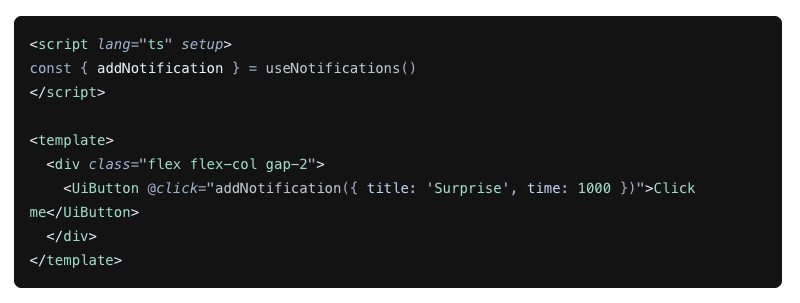
\includegraphics[width=\textwidth]{images/shiki}
  \caption{Zvýraznění kódu pomocí Shiki} \label{picture:shiki}
\end{figure}

\subsection{Headless UI}
Nestylované, přístupné UI komponenty, navržené tak, aby se jednoduše používaly s Tailwind CSS. \cite{HeadlessUI}

Headless UI je sada přístupných UI komponent, které jsou navrženy tak, aby byly snadno integrovatelné do jakéhokoliv designu nebo frontendového frameworku. Tato knihovna poskytuje základní funkční strukturu pro běžné UI prvky, jako jsou rozbalovací menu, přepínače a dialogová okna, ale neobsahuje žádné vlastní styly, což umožňuje vývojářům plně ovládat vzhled těchto komponent. Headless UI je ideální pro projekty, které vyžadují vysokou míru přizpůsobení a chtějí používat specifický designový jazyk bez nutnosti bojovat s předdefinovanými styly. Komponenty jsou navrženy s ohledem na přístupnost, což zajišťuje, že aplikace jsou použitelné pro širokou škálu uživatelů, včetně těch s omezenými schopnostmi. Headless UI tak usnadňuje vytváření robustních a esteticky příjemných webových aplikací, které jsou zároveň přístupné a uživatelsky přívětivé.

V této diplomové práci je Headless UI použit pro tvorbu základních UI komponent, jako jsou modální okna, navigační lišty či další prvky. Tato knihovna poskytuje flexibilitu a kontrolu nad vzhledem komponent, což je důležité pro jednoduché úpravy a rozšíření.

\subsection{Floating UI}
Floating UI je Javascriptová knihovna navržená pro pozicování plovoucích prvků, jako jsou tooltipy, popovery a dropdown menu, a umožňuje také vytváření interakcí pro tyto prvky. Knihovna se zaměřuje na robustní ukotvení absolutně pozicovaných plovoucích prvků vedle referenčních prvků s funkcemi, které zabraňují kolizím s okrajem zobrazení, čímž zajišťuje, že plovoucí prvky zůstanou vždy viditelné a optimálně umístěné.

Floating UI podporuje různé platformy včetně webu, React, React Native a Vue, a je vysoce modulární, což umožňuje vývojářům použít jen tolik funkcionality, kolik potřebují, což může vést k optimalizaci velikosti balíčku. Dále je knihovna navržena tak, aby byla flexibilní a umožňovala snadnou integraci bez omezení na specifické technologie nebo frameworky. \cite{FloatingUI}

V této diplomové práce se Floating UI používá pro tvorbu interaktivních prvků, jako jsou tooltipy a popovery, které zvyšují uživatelskou interaktivitu a zlepšují uživatelskou zkušenost. Důležité je především zabránění přetékání prvků mimo obrazovku a zajištění, že plovoucí prvky jsou vždy viditelné a snadno přístupné.

\subsection{Embla Carousel}
Embla Carousel je malá, open source knihovna pro Javascript, která se zaměřuje na tvorbu pohyblivých prvků, jako jsou carousely, s vysokou přesností pohybu a skvělou reakcí na gesta. Tato knihovna je navržena tak, aby byla nezávislá na jiných knihovnách a nevyžaduje žádné další závislosti. \cite{EmblaCarousel}

Embla Carousel nabízí možnost snadné integrace do různých frameworků jako React, Vue, Svelte a Solid, díky čemuž je flexibilní pro různé typy projektů. Využívá moderní CSS vlastnosti, jako je flexbox, pro definování velikosti a mezer mezi prvky a podporuje i pokročilé funkce, jako je automatické přehrávání a responzivní nastavení.

K dispozici jsou různé pluginy, které rozšiřují základní funkčnost, včetně možností pro automatické přehrávání, auto-scroll, a adaptaci výšky. Embla také poskytuje rozsáhlé API pro pokročilé manipulace a přizpůsobení carouselů, což umožňuje vývojářům plně ovládat chování a vzhled carouselů podle potřeb projektu.

V této práci je Embla Carousel použit pro tvorbu carousel komponenty. Díky vysoké flexibilitě poskytuje nepřeberné možnosti konfigurace a přizpůsobení.

\section{CLI}
Tato sekce se věnuje technologiím a nástrojům, které byly použity pro vývoj CLI pro instalaci komponent.

\subsection{Commander.js}
Commander.js je oblíbená knihovna pro Node.js, která usnadňuje vytváření příkazových řádkových rozhraní (CLI). Umožňuje vývojářům definovat příkazy, volby a parametry pro jejich aplikace v jednoduchém a strukturovaném formátu. Commander.js poskytuje funkce, jako je automatické generování nápovědy, parsování příkazů a argumentů, a podporu pro subpříkazy, což umožňuje vývojářům snadno rozšiřovat funkčnost svých aplikací bez nutnosti psát rozsáhlý kód pro zpracování vstupů. Díky své flexibilitě a jednoduchosti použití se Commander.js stal standardním nástrojem pro mnoho projektů založených na Node.js. \cite{CommanderJS}

V této diplomové práci je Commander.js použit pro vytvoření CLI pro instalaci komponent.

Jako alternativa se nabízí Citty z ekosystému UnJS. Má podobné funkce jako Commander, avšak v době tvorby této práce byla tato knihovna v rané fázi vývoje a nebyla dostatečně stabilní pro použití v produkčním prostředí. \cite{Citty}

\subsection{Ora}
Ora je minimalistická a efektivní knihovna pro Node.js, která umožňuje vývojářům přidat elegantní indikátory načítání (tzv. spinners) do jejich CLI. Tyto indikátory jsou užitečné pro zobrazování stavu dlouhotrvajících operací, aniž by uživatele zatěžovaly nadměrnými informacemi. Ora nabízí širokou škálu přednastavených stylů a umožňuje také snadnou personalizaci, včetně změny textu, barvy a symbolů spinneru. Tato knihovna je oblíbená pro svou snadnou integraci a schopnost výrazně zlepšit uživatelskou zkušenost CLI aplikací tím, že poskytuje okamžitou vizuální zpětnou vazbu během procesů, které mohou trvat několik sekund nebo i déle. \cite{Ora}

V této diplomové práci je Ora použit pro zobrazení indikátorů načítání během procesů instalace komponent.

\subsection{Prompts}
Prompts je knihovna pro Node.js, která umožňuje vývojářům snadno vytvářet interaktivní CLI. S pomocí této knihovny je možné efektivně spravovat uživatelské vstupy pomocí různých typů dotazů, jako jsou text, heslo, potvrzení a výběr z možností. Prompts podporuje asynchronní logiku, umožňuje validaci vstupů a podmíněné zobrazení dotazů, což vývojářům poskytuje flexibilitu pro vytváření složitějších scénářů interakcí. Tato knihovna je oblíbená pro svou jednoduchost, moderní API a minimální závislosti, což ji činí ideální volbou pro projekty, kde je potřeba rychle a efektivně zpracovávat uživatelské vstupy. \cite{Prompts}

V této diplomové práci je knihovna Prompts použita pro interaktivní získávání informací od uživatele během procesu instalace komponent.

\subsection{Execa}
Execa je moderní knihovna pro Node.js, která zjednodušuje práci s externími procesy a příkazy shellu. Tato knihovna je navržena tak, aby vylepšila standardní Node.js metodu child\_process a poskytla lepší zkušenost s pokročilými funkcemi, jako je podpora asynchronních operací, vylepšená oblast viditelnosti výstupů procesů a lepší manipulace s chybami. Execa umožňuje snadné spouštění shell příkazů a jejich sledování v reálném čase, což je zvláště užitečné v automatizovaných skriptech a nástrojích pro vývoj. Díky execa lze také snadno získat textový výstup příkazů, což umožňuje vývojářům efektivně zpracovávat data bez nutnosti manuálního parsingu. \cite{Execa}

V této diplomové práci je knihovna Execa použita pro instalaci závislostí během instalace komponent.

\subsection{Zod}
Zod je knihovna pro Typescript, která slouží k vytváření schémat a validaci dat s cílem zajistit správnost typů během kompilace i za běhu. Zod umožňuje vývojářům definovat strukturu dat pomocí silného typového systému Typescriptu, což vede ke snížení chyb způsobených neplatnými daty. Jednou z klíčových výhod Zodu je, že integrované validace se automaticky odrážejí ve vygenerovaných typech, což znamená, že jakékoli data splňující validaci jsou automaticky správně typována. Tato knihovna také podporuje složitější validační struktury, včetně vnořených objektů, pole, volitelných polí a unie typů, což ji činí ideálním řešením pro aplikace, které vyžadují přísnou kontrolu vstupních dat. \cite{Zod}

V této diplomové práci je knihovna Zod použita pro definici schémat a validaci dat během procesu instalace komponent.

\subsection{Tsup}
Tsup je minimalistický a rychlý bundler pro Typescript a Javascript, postavený na technologii esbuild. Umožňuje vývojářům efektivně sestavovat své projekty s výrazným zlepšením v rychlosti sestavení oproti tradičním nástrojům jako je Webpack nebo Rollup. Tsup nabízí jednoduché CLI s několika konfiguračními možnostmi, což usnadňuje jeho používání a integraci do různých projektů. Mezi klíčové funkce patří podpora pro tree-shaking, generování deklarací Typescript, a podpora pro ESM a CommonJS moduly. Díky své závislosti na esbuild, tsup poskytuje nejen rychlost, ale také efektivitu při minimalizaci a optimalizaci výsledného kódu.  \cite{Tsup}

V této diplomové práci je tsup použit pro sestavení výsledného balíčku CLI pro instalaci komponent.

\section{Infrastruktura}
Tato sekce se věnuje technologiím a nástrojům, které byly použity pro správu kódu a jeho následné nasazení.

\subsection{pnpm workspaces}
pnpm workspaces jsou součástí správce balíčků pnpm, které umožňují efektivní správu více balíčků v rámci jednoho repozitáře (monorepo). Tato funkcionalita usnadňuje sdílení závislostí mezi projekty, což minimalizuje redundanci a zvyšuje efektivitu správy kódu. Workspaces podporují spojení více projektů pod jednou střechou s jednotnou správou závislostí, což je ideální pro velké projekty s mnoha podprojekty nebo knihovnami. Díky pnpm workspaces lze jednoduše instalovat závislosti pro všechny workspaces najednou, zatímco se zachovává úspora místa na disku a rychlost díky strategii pnpm pro sdílení závislostí. \cite{PnpmWorkspaces}

V této diplomové práci jsou pnpm workspaces použity pro efektivní správu kódu v rámci monorepozitáře. Díky tomu, že jsou oba projekty (CLI a dokumentace) součástí jednoho repozitáře, je možné jednoduše testovat jejich propojení bez nutnosti stahování více repozitářů a jejich propojování, což zjednodušuje vývoj a údržbu.


\subsection{Changesets}
Changesets je nástroj, který pomáhá spravovat, verzovat a zveřejňovat změny v projektech s mnoha balíčky, typicky v monorepozitářích. Tento systém umožňuje vývojářům přidávat \uv{changeset}~soubory do git repozitáře, které popisují změny v balíčcích a jejich dopad na semantické verzování. Když přichází čas na vydání nové verze, Changesets automaticky generuje changelogy a aktualizuje verze balíčků podle pravidel semantického verzování. Tato metoda zajišťuje, že uživatelé knihovny mají jasné informace o tom, co každá verze zahrnuje. Changesets tak přináší transparentnost a předvídatelnost do procesu vývoje softwaru, což je zvláště cenné v prostředích, kde spolupracuje mnoho vývojářů. \cite{Changesets}

V této diplomové práci je Changesets použit pro správu změn a verzování balíčků v rámci monorepozitáře. Tento nástroj zajišťuje, že všechny změny jsou správně dokumentovány a verzovány, což usnadňuje vydávání nových verzí.

\subsection{npm}
npm (Node Package Manager) je systém pro správu balíčků, který je standardně používán pro Javascriptový runtime Node.js. npm umožňuje vývojářům snadno sdílet a spravovat závislosti kódu v jejich Javascriptových projektech. Na oficiálních stránkách npm je dostupný obrovský repozitář obsahující přes 2,5 milionu balíčků, které může komunita využívat a přispívat do nich (v rámci open source repozitářů). Balíčky mohou obsahovat vše od malých knihoven až po komplexní frameworky. \cite{Npm}

Přidání balíčku do npm je relativně jednoduchý proces, který začíná vytvořením účtu. Po přihlášení může vývojář vytvořit nový balíček pomocí příkazu npm init, který vede k nastavení balíčku včetně jeho názvu, verze, a závislostí. Po konfiguraci lze balíček publikovat na npm pomocí příkazu npm publish. Je důležité správně nastavit soubor package.json, který obsahuje metadata a závislosti balíčku. Vývojáři musí také zvážit licencování a další právní aspekty, aby byl jejich kód správně chráněn a licencován pro užití ostatními.

npx je nástroj přibalený s npm, který zjednodušuje spouštění balíčků nainstalovaných ve vašem Node.js prostředí nebo přímo z npm repozitáře bez nutnosti je explicitně instalovat. npx je užitečný zejména pro jednorázové spouštění balíčků nebo pro vyzkoušení nových nástrojů bez zatěžování vašeho lokálního vývojového prostředí. Když spustíte příkaz pomocí npx, například npx nuxi init my-app, npx automaticky stáhne potřebný balíček a jeho závislosti, spustí jej a po dokončení operace tyto dočasné instalace odstraní, čímž udržuje vaše prostředí čisté.

V této diplomové práci je npm použito pro publikaci balíčku CLI pro instalaci komponent. Poté se pro jeho spuštění využívá npx.

\subsection{Github}
GitHub je jedna z největších a nejznámějších platforem pro správu softwarových projektů a verzování kódu pomocí systému Git. Umožňuje vývojářům hostovat a verzovat kód, spravovat projekty a sestavovat software společně s miliony dalších uživatelů po celém světě. GitHub poskytuje nástroje pro kolaborativní vývoj, jako jsou pull requesty (připojení nového kódu do dalších větví), správa větví a issues pro každý projekt. Platforma se stala populárním nástrojem pro open source projekty, ale je rovněž populární mezi společnostmi pro soukromý vývoj softwaru díky svým robustním funkcím pro správu přístupu a integraci s různými externími službami. Dále, GitHub rozšiřuje své funkce o GitHub Actions, což jsou automatizační nástroje pro CI/CD procesy, které umožňují automatizovat testování a nasazování aplikací přímo z repozitářů na GitHubu. \cite{Github}

V této diplomové práci je GitHub použit pro správu kódu a verzování projektu. Díky GitHub Actions jsou automatizovány procesy testování a nasazování aplikace.

\subsection{Cloudflare}
Cloudflare je společnost poskytující širokou škálu služeb zaměřených na zlepšení bezpečnosti a výkonu internetových aplikací a webů. Cloudflare funguje primárně jako CDN (Content Delivery Network), které pomáhá zrychlit načítání webových stránek tím, že ukládá obsah na geograficky rozptýlených serverech a nabízí jej uživatelům z nejbližší možné lokality. Kromě toho Cloudflare poskytuje řešení pro ochranu před DDoS útoky, zabezpečení webových aplikací (WAF), bezpečné DNS služby a optimalizaci provozu. \cite{Cloudflare}

Cloudflare Developer Platform nabízí vývojářům nástroje a API pro vytváření, testování a nasazování aplikací přímo na jejich edge network. Tato platforma zahrnuje řadu produktů jako Workers (serverless computing), který umožňuje vývojářům spouštět Javascript a WebAssembly kód na Cloudflare servery blízko uživatelů, což výrazně snižuje latenci a zvyšuje výkon aplikací. Avšak cenou za tuto rychlost je nutnost dodržovat určitá pravidla a omezit se na určité technologie, které jsou podporovány edge runtimem. \cite{CloudflareDeveloperPlatform}

Cloudflare Pages je platforma pro hosting statických webů a web aplikací, která je integrovaná přímo do Cloudflare infrastruktury. Je ideální pro projekty, které vyžadují rychlé načítání a globální dostupnost bez nutnosti spravovat serverovou infrastrukturu. Pages podporuje moderní frameworky a build nástroje jako React, Vue, Angular, včetně Nuxtu, a mnoho dalších, a automaticky konfiguruje HTTPS a SSL pro všechny nasazené stránky. \cite{CloudflarePages}

Hlavní výhody Cloudflare Pages zahrnují:

\begin{itemize}
    \item Snadné nasazení: Cloudflare Pages jsou navrženy pro snadnou integraci s GitHubem, což umožňuje vývojářům nasadit své aplikace přímo z repozitářů.
    \item Automatizované buildy: Každý push do hlavní větve repozitáře automaticky spustí proces sestavení a nasazení nové verze aplikace.
    \item Bezpečnost a rychlost: Využívání Cloudflare CDN a bezpečnostních funkcí zajišťuje, že aplikace jsou nejen rychle dostupné odkudkoli, ale také chráněné před běžnými útoky.
\end{itemize}

V této diplomové práci jsou Cloudflare Pages použity pro nasazení dokumentace a ukázek. Díky integraci s GitHubem je možné jednoduše nasadit novou verzi aplikace po každé změně v repozitáři.

%! Author = Vojta
%! Date = 21.1.2024

\chapter{Návrh}

\section{Úvod}
Návrh je důležitým krokem v procesu vývoje, který předchází samotné implementaci a testování. V této kapitole bude podrobně rozebrán postup a myšlenkové procesy, které vedou k vytvoření sbírky komponent přívětivé jak pro uživatele, tak pro vývojáře. Nejprve bude popsán vývoj a struktura dokumentace, která je nezbytná pro správné použití a rozšíření UI kolekce, dále návrh samotných komponent a příprava Figma kitu, který slouží jako most mezi designéry a vývojáři. Také bude vysvětlen význam a využití bloků, které umožňují rychlejší a efektivnější vývoj webových aplikací. Nakonec bude popsán návrh CLI, které umožňuje snadné přidávání komponent do existujících projektů.

\section{Dokumentace}
Součástí každého softwarového projektu by měla být kvalitní dokumentace (ačkoliv se tak často neděje). Pro účely této sbírky znovupoužitelných UI komponent je potřeba připravit dokumentaci, která nejen vysvětluje jak používat jednotlivé komponenty, ale také poskytuje ucelený pohled na architekturu a filozofii za celým projektem. Tato sekce se zabývá obsahem dokumentace a její strukturou.

\subsection{Obsah dokumentace}
Hlavním cílem dokumentace je poskytnout vývojářům všechny potřebné informace.

\begin{description}
  \item[Úvod do principů a filozofie knihovny] Vysvětlení v čem se knihovna liší od typických UI knihoven.
  \item[Návod k použití] Průvodce krok za krokem jak začít využívat komponenty knihovny.
  \item[Podpůrné materiály] Doprovodné zdroje, například Figma kit a tipy pro řešení problémů.
  \item[Přehled komponent] Detailní popis každé komponenty, včetně jejího účelu, možností konfigurace a příkladů použití.
\end{description}

Dokumentace bude rozdělena do dvou hlavních sekcí: \uv{Getting Started} a \uv{Components}. Sekce \uv{Getting Started} bude poskytovat uživatelům všechny základní informace potřebné pro rychlý start s knihovnou, včetně instalace, konfigurace a prvních kroků s komponentami. To pomůže novým uživatelům snadno se orientovat v možnostech knihovny a začít s jejím používáním. Sekce \uv{Components} se bude zabývat detailním popisem jednotlivých komponent, včetně jejich vlastností, možností přizpůsobení a příkladů použití.

\subsection{Dokumentace konkrétních komponent}
Stránka dokumentace pro každou konkrétní komponentu bude jasně strukturovaná a poskytuje ucelené informace, které usnadní její použití. Na začátku stránky bude uveden název komponenty a pod ním krátký popis, který objasňuje, k čemu komponenta slouží. Bude následovat sekce s ukázkou komponenty, doplněná o příslušný zdrojový kód, který bude ilustrovat, jak lze komponentu použít. Návod k instalaci bude popisovat, jak komponentu přidat do projektu, ať už pomocí CLI nástroje nebo prostřednictvím manuálního kopírování kódu. Na stránce vývojáři naleznou také seznam props a slotů, které umožňují přizpůsobit komponentu specifickým potřebám. Stránka může dále obsahovat další poznámky a varování ohledně specifik komponenty, jako jsou potenciální chyby, omezení, nebo doporučené postupy.

\section{Figma Kit}
Figma Kit je vyvinut s cílem poskytnout designérům a vývojářům snadno použitelnou sadu komponent, které jim umožní efektivně navrhovat a prototypovat aplikace. Kit obsahuje komponenty UI kolekce, přesně tak, jak jsou definovány ve finální implementaci, což zajišťuje, že designy jsou plně kompatibilní s konečnou implementací. Připravené jsou komponenty jako tlačítka, inputy, plovoucí prvky a mnoho dalšího, což designérům umožňuje sestavit uživatelské rozhraní rychle a s vysokou mírou přesnosti.

Pro vývojáře je pak snadné převést designy vytvořené v Figmě do kódu, protože mohou snadno identifikovat, které komponenty mají být použity. Díky definovaným proměnným lze snadno přizpůsobit barvy, velikosti a další vlastnosti komponent, které vývojáři mohou specifikovat v rámci projektu.

U každé komponenty se nachází odkaz do dokumentace, kde mohou jak designéři, tak vývojáři najít podrobné informace o tom, k čemu komponenta je a jaké jsou její možnosti.

\begin{figure}[H]
  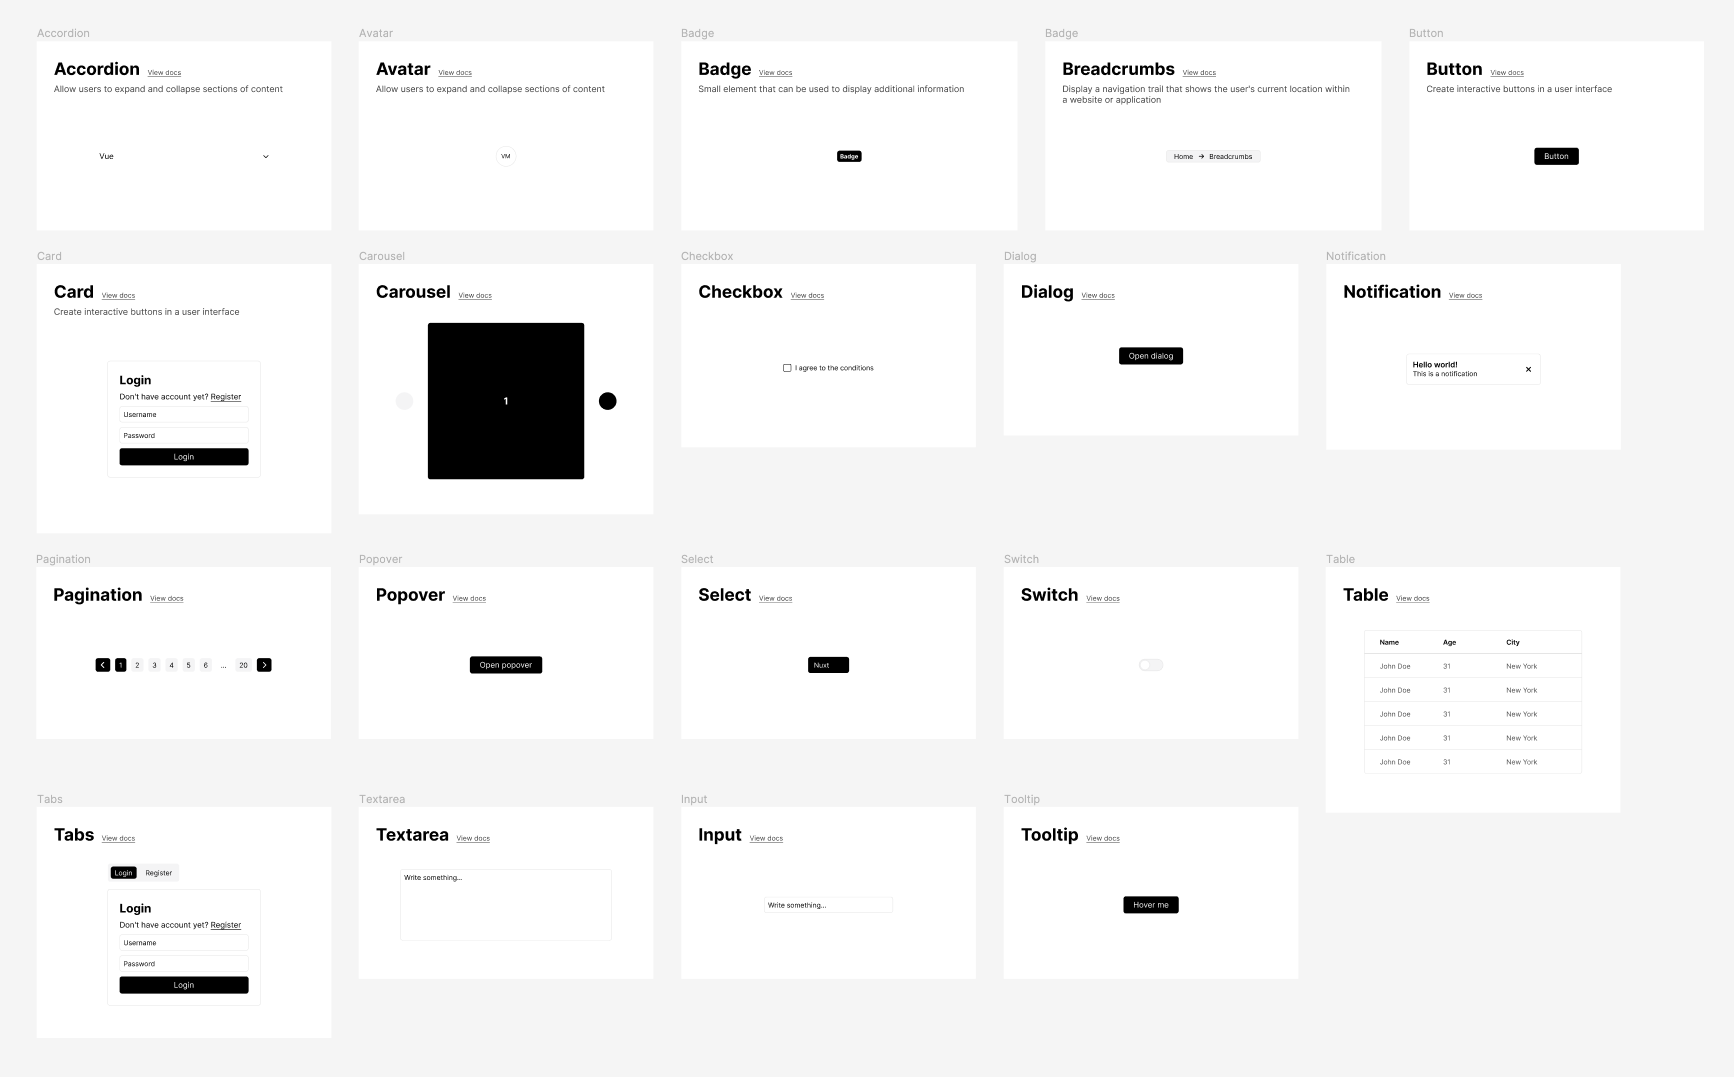
\includegraphics[width=\textwidth]{images/figma-kit}
  \caption{Komponenty ve Figmě} \label{picture:figma-kit}
\end{figure}

\section{Komponenty}
Výběr těchto komponent byl založen na jejich základní funkčnosti a častém využití ve webových aplikacích. Každá z těchto komponent přináší konkrétní užitečné vlastnosti, které zlepšují uživatelský zážitek a zjednodušují vývojový proces. Tento soubor základních komponent vytváří pevný základ pro další rozšiřování sbírky. V budoucnu bude sbírka doplněna o další komponenty, které budou reagovat na specifické potřeby a požadavky vývojářů.

\subsection{Accordion}
Accordion je komponenta určená k zobrazení a skrytí obsahu v rozbalovacích sekcích. Umožňuje uživatelům zobrazit pouze relevantní část informací a zbytek skrýt, čímž šetří místo na obrazovce a zvyšuje přehlednost. Accordion se často používá pro často kladené otázky (FAQ) nebo detaily produktů.

\begin{figure}[H]
  \centering
  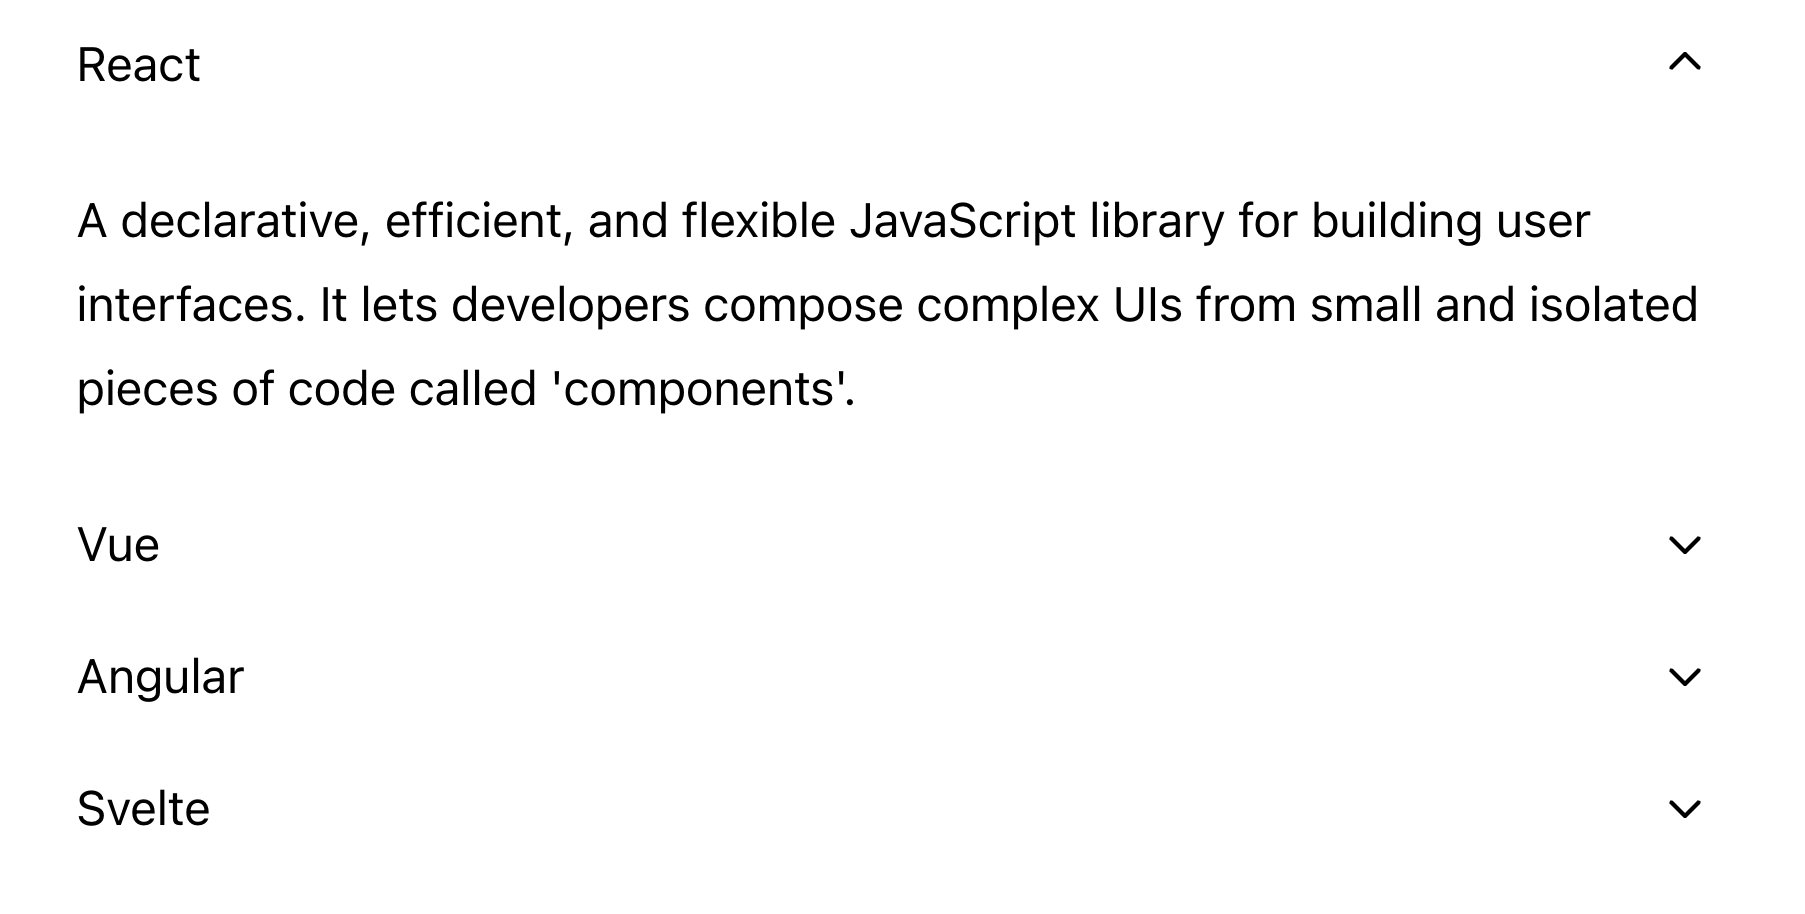
\includegraphics[width=10cm]{images/accordion}
  \captionsetup{justification=centering,margin=2cm}
  \caption{Accordion} \label{picture:accordion}
\end{figure}

\subsection{Avatar}
Avatar je vizuální reprezentace uživatele, obvykle v podobě kruhového nebo čtvercového obrázku. Používá se k identifikaci uživatelů v aplikacích, například v uživatelských profilech, seznamu kontaktů nebo diskuzních fórech. Avatar může obsahovat iniciály uživatele, ikonu nebo fotografii.

\begin{figure}[H]
  \centering
  
\includegraphics[width=2cm]{images/avatar}
  \captionsetup{justification=centering,margin=2cm}
  \caption{Avatar} \label{picture:avatar}
\end{figure}

\subsection{Badge}
Badge je komponenta používaná k zobrazení malého označení nebo indikátoru, který poskytuje dodatečnou informaci. Typickým použitím je například zobrazení štítků, počtu nepřečtených zpráv, oznámení nebo označení nových funkcí v aplikaci.

\begin{figure}[H]
  \centering
  
\includegraphics[width=2cm]{images/badge}
  \captionsetup{justification=centering,margin=2cm}
  \caption{Badge} \label{picture:badge}
\end{figure}

\subsection{Breadcrumbs}
Breadcrumbs slouží k navigaci a orientaci uživatelů na webových stránkách nebo v aplikacích. Zobrazuje hierarchii stránek, což uživatelům umožňuje rychle se vrátit na předchozí úrovně nebo domovskou stránku. Breadcrumbs zlepšují uživatelskou zkušenost tím, že usnadňují navigaci v komplexních strukturách.

\begin{figure}[H]
  \centering
  
\includegraphics[width=5cm]{images/breadcrumbs}
  \captionsetup{justification=centering,margin=2cm}
  \caption{Breadcrumbs} \label{picture:breadcrumbs}
\end{figure}

\subsection{Button}
Button je základní interaktivní komponenta, která umožňuje uživatelům provádět akce, jako je odeslání formuláře, zahájení procesu nebo navigace na jinou stránku. Buttony mohou mít různé styly a velikosti, aby odpovídaly specifickým požadavkům aplikace nebo designu.

\begin{figure}[H]
  \centering
  
\includegraphics[width=3cm]{images/button}
  \captionsetup{justification=centering,margin=2cm}
  \caption{Button} \label{picture:button}
\end{figure}

\subsection{Card}
Card je vizuální komponenta, která obklopuje obsah a poskytuje kontext. Karty jsou často používány k organizaci informací do samostatných bloků, které mohou obsahovat obrázky, texty a akční tlačítka. Cards se využívají v dashboardech, produktech nebo profilech uživatelů.

\begin{figure}[H]
  \centering
  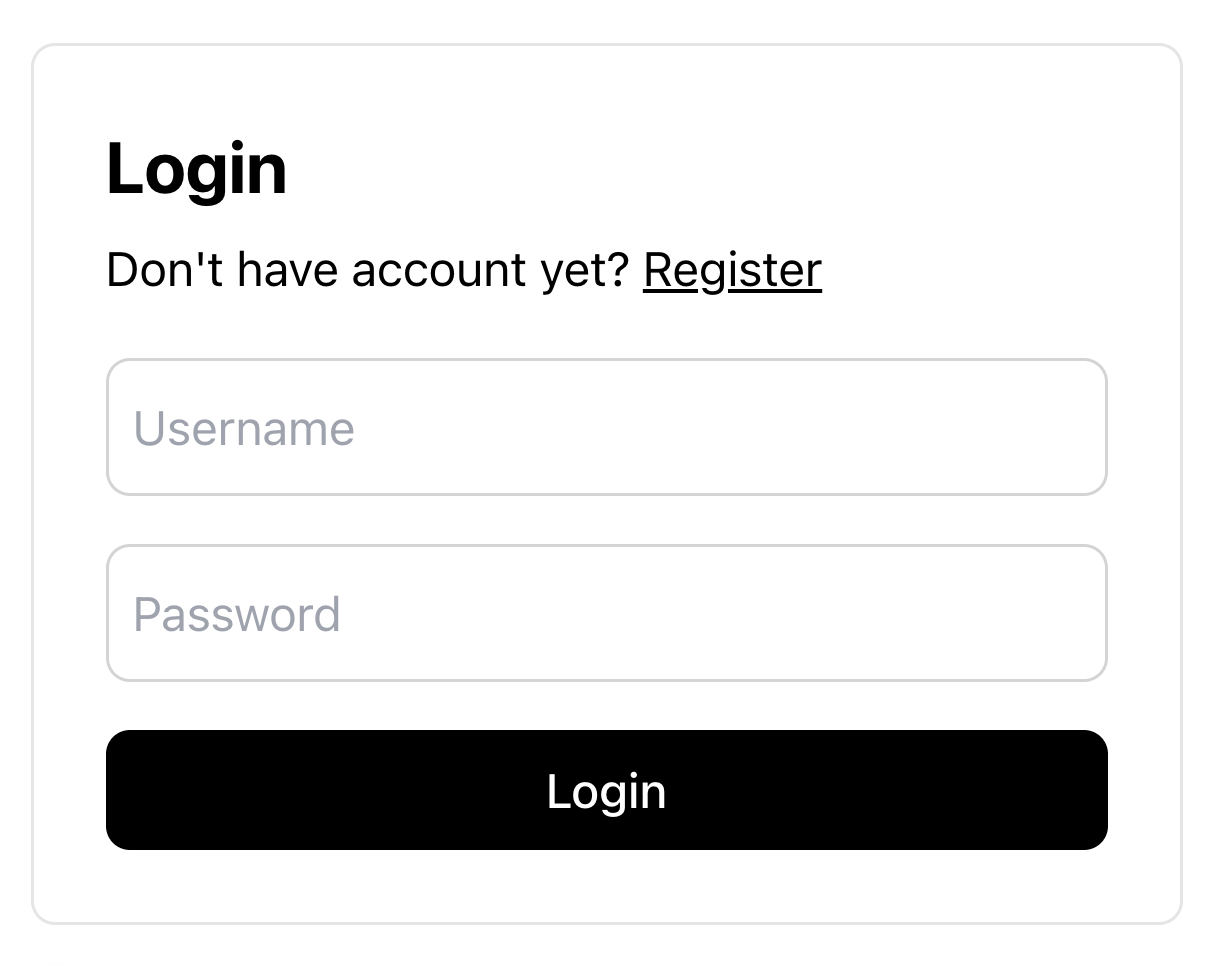
\includegraphics[width=7cm]{images/card}
  \captionsetup{justification=centering,margin=2cm}
  \caption{Card} \label{picture:card}
\end{figure}

\subsection{Carousel}
Carousel je komponenta umožňující zobrazení více položek (obrázků, karet) v rotující nebo posuvné formě. Umožňuje efektivně využít prostor a zobrazit více obsahu na omezené ploše, což je ideální pro prezentaci galerií, doporučených produktů nebo novinek.

\begin{figure}[H]
  \centering
  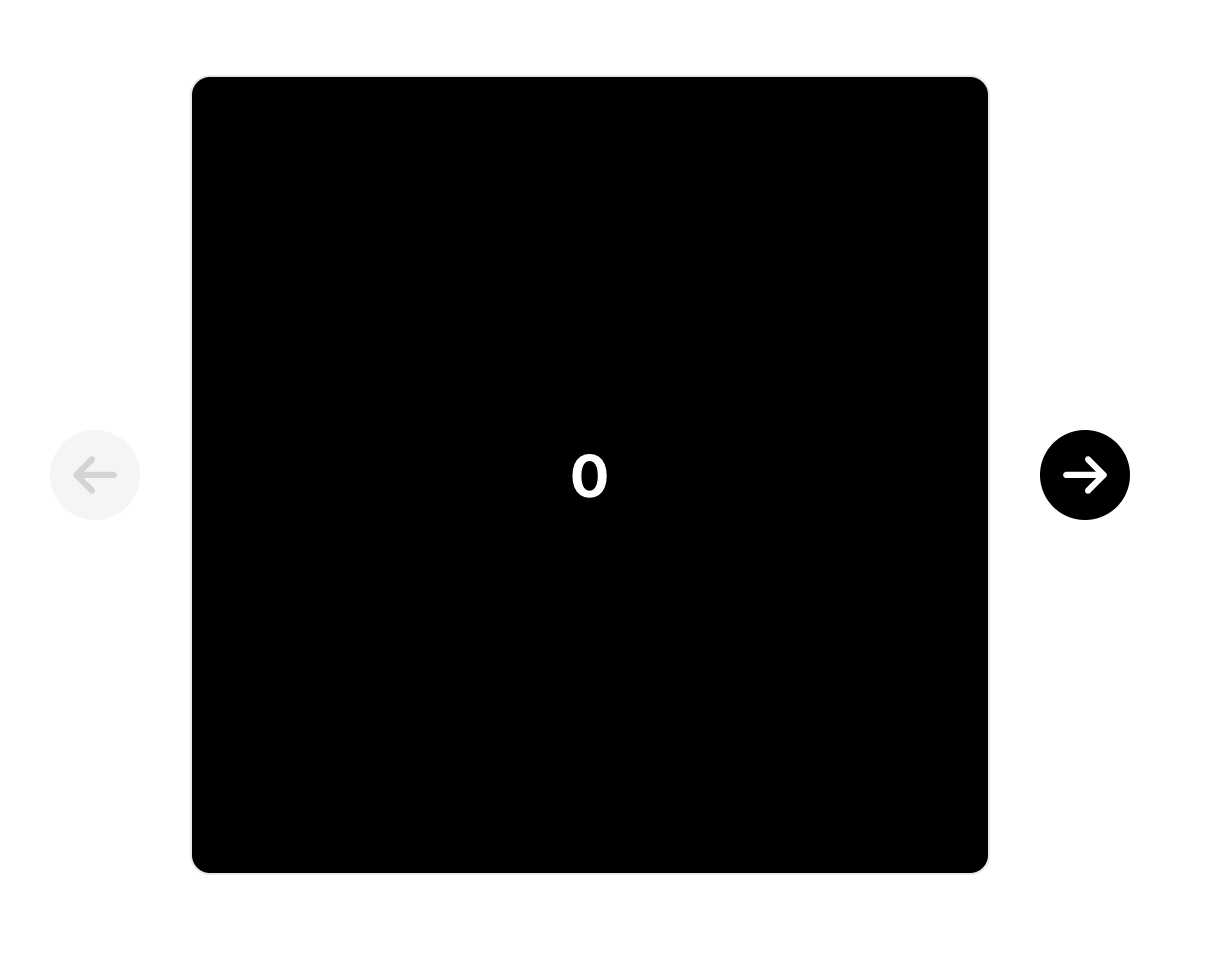
\includegraphics[width=7cm]{images/carousel}
  \captionsetup{justification=centering,margin=2cm}
  \caption{carousel} \label{picture:carousel}
\end{figure}

\subsection{Checkbox}
Checkbox je vstupní komponenta, která umožňuje uživatelům vybrat jednu nebo více možností z nabídky. Používá se v formulářích, nastaveních a dalších interaktivních prvcích, kde je potřeba více výběrů.

\begin{figure}[H]
  \centering
  
\includegraphics[width=5cm]{images/checkbox}
  \captionsetup{justification=centering,margin=2cm}
  \caption{checkbox} \label{picture:checkbox}
\end{figure}

\subsection{Dialog}
Dialog je modální okno, které se objevuje nad hlavním obsahem stránky, aby poskytlo důležité informace nebo vyžádalo potvrzení akce od uživatele. Dialogy jsou používány pro potvrzovací zprávy, formuláře nebo upozornění, která vyžadují okamžitou pozornost uživatele.

\subsection{Icon}
Icon je grafický symbol reprezentující akci, objekt nebo koncept. Ikony se používají ke zlepšení vizuální komunikace v uživatelských rozhraních, často jako doplněk textových popisků. Mohou být použity v tlačítkách, navigačních lištách nebo jako vizuální indikátory. Pro použití ikon existuje modul Nuxt Icon, který zpřístupňuje mnoho ikon pro efektivní použití v aplikacích. Tento modul je velmi pokročilý a proto je v dokumentaci doporučené jej použít.

\subsection{Loading}
Loading je komponenta, která indikuje probíhající proces nebo načítání obsahu. Pomáhá uživatelům pochopit, že akce je v procesu a vyžaduje čas. Loading indikátory mohou mít různé formy, například točící se kolečko, prodlužující se pruh nebo blikající tečky.

\begin{figure}[H]
  \centering
  \subfloat{
\includegraphics[width=2cm]{images/loading-circle}}
  \hspace{1cm}
  \subfloat{
\includegraphics[width=3cm]{images/loading-dots}}\\
  \subfloat{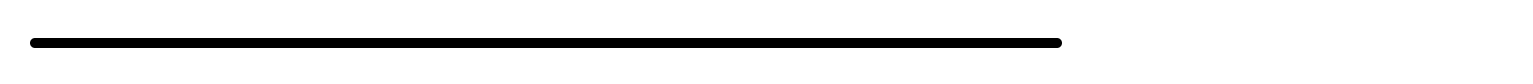
\includegraphics[width=10cm]{images/loading-progress}}
  \captionsetup{justification=centering,margin=2cm}
  \caption{Loading}
\end{figure}

\subsection{Notification}
Notification je komponenta pro zobrazení krátkých zpráv nebo upozornění uživatelům. Může informovat o úspěšných akcích, varováních, chybách nebo nových událostech. Notifikace mohou být dočasné nebo trvalé, a obvykle se zobrazují v rohu obrazovky.

\begin{figure}[H]
  \centering
  
\includegraphics[width=7cm]{images/notification}
  \captionsetup{justification=centering,margin=2cm}
  \caption{notification} \label{picture:notification}
\end{figure}

\clearpage

\subsection{Pagination}
Pagination je komponenta, která rozděluje obsah do více stránek a poskytuje ovládací prvky pro navigaci mezi nimi. Používá se v aplikacích a na webových stránkách s velkým množstvím dat, aby se usnadnila jejich přehlednost a navigace.

\begin{figure}[H]
  \centering
  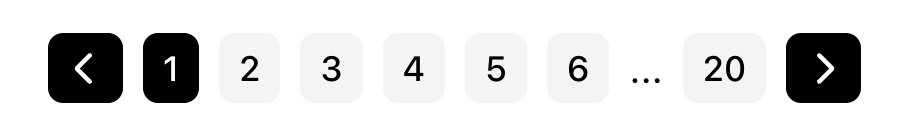
\includegraphics[width=7cm]{images/pagination}
  \captionsetup{justification=centering,margin=2cm}
  \caption{pagination} \label{picture:pagination}
\end{figure}

\subsection{Popover}
Popover je komponenta, která zobrazuje dodatečný obsah v malém okně, které se objevuje pod obsahem po interakci uživatele. Popover se často používá pro kontextové nabídky, tipy nebo formuláře, které vyžadují uživatelovu pozornost, aniž by opustil aktuální stránku.

\begin{figure}[H]
  \centering
  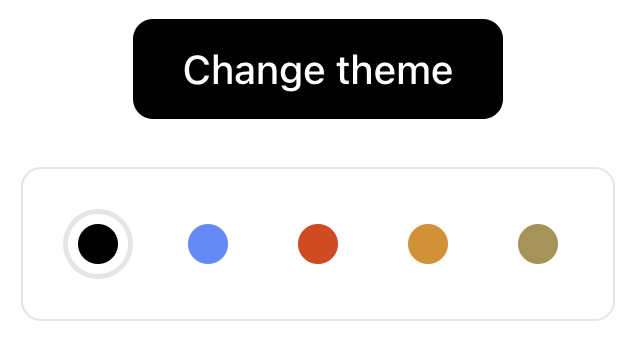
\includegraphics[width=5cm]{images/popover}
  \captionsetup{justification=centering,margin=2cm}
  \caption{popover} \label{picture:popover}
\end{figure}

\subsection{Select}
Select je vstupní komponenta umožňující uživatelům vybrat jednu možnost z rozbalovací nabídky. Používá se v formulářích a nastaveních, kde je potřeba vybrat z předdefinovaného seznamu hodnot. Select komponenty mohou být jednoduché nebo víceúrovňové.

\begin{figure}[H]
  \centering
  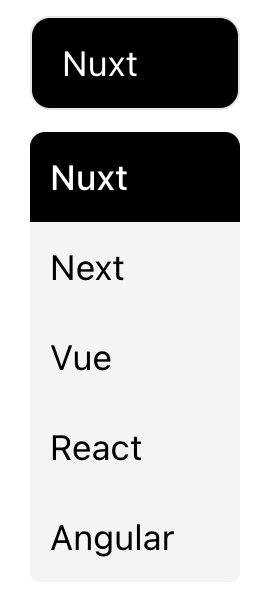
\includegraphics[width=3cm]{images/select}
  \captionsetup{justification=centering,margin=2cm}
  \caption{select} \label{picture:select}
\end{figure}

\subsection{Sidebar}
Sidebar je vertikální panel, který poskytuje navigaci nebo další obsah vedle hlavního obsahu stránky. Sidebary se používají pro menu, seznamy položek nebo další interaktivní prvky, které zůstávají přístupné během procházení hlavního obsahu.

\subsection{Switch}
Switch je komponenta, která umožňuje uživatelům přepínat mezi dvěma stavy, obvykle zapnuto a vypnuto. Používá se pro nastavení, která mají binární volbu, jako je povolení nebo zakázání funkcí.

\begin{figure}[H]
  \centering
  \subfloat{
\includegraphics[width=2cm]{images/switch}\label{picture:documentation:switch}}
  \hspace{1cm}
  \subfloat{
\includegraphics[width=2cm]{images/switch-on}\label{picture:documentation:switch-on}}
  \captionsetup{justification=centering,margin=2cm}
  \caption{Switch}
\end{figure}

\subsection{Table}
Table je komponenta pro zobrazení strukturovaných dat ve formě tabulky. Tabulky se používají k organizaci informací do řádků a sloupců, což umožňuje snadné srovnání a analýzu dat. Jsou běžně používány v dashboardech, reportech a dalších datově orientovaných aplikacích.

\begin{figure}[H]
  \centering
  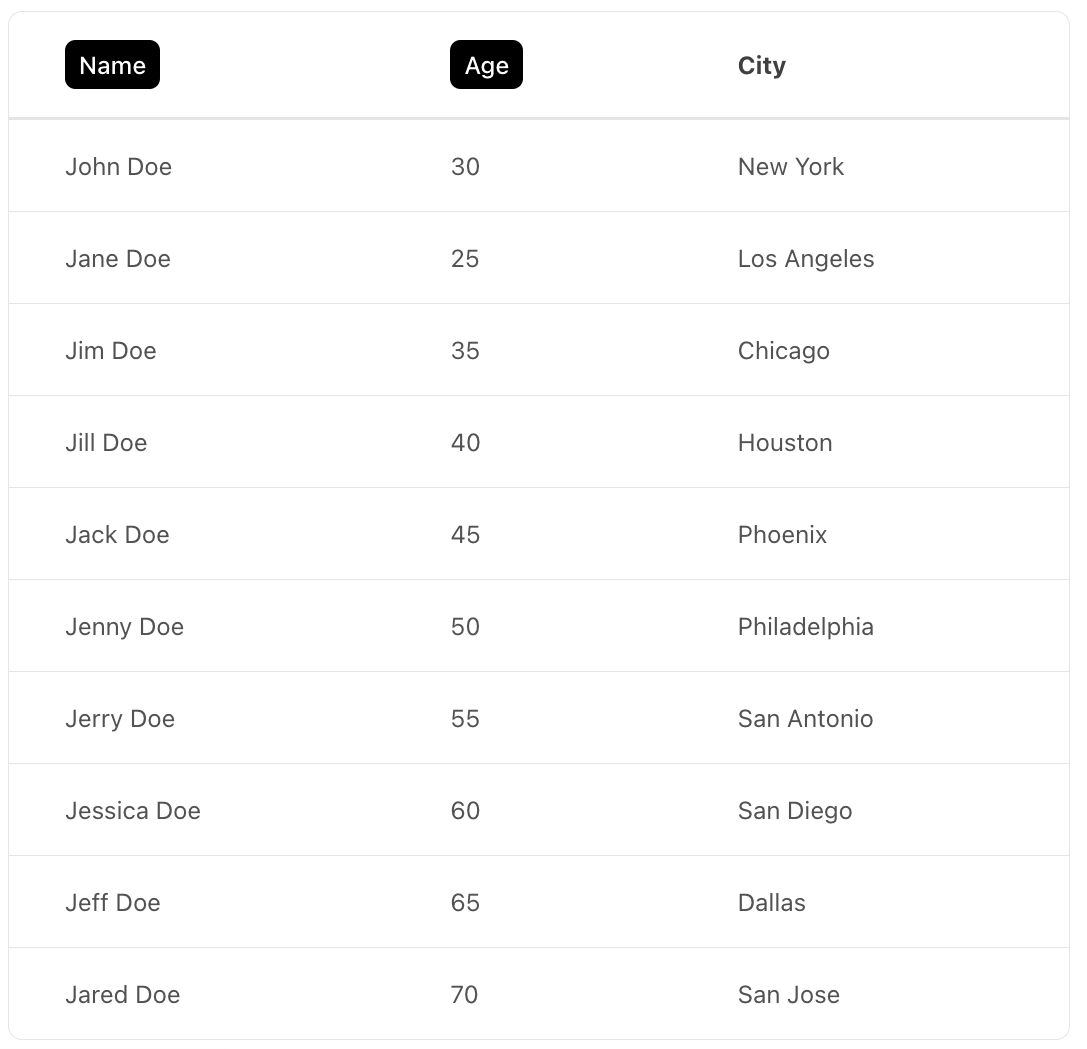
\includegraphics[width=10cm]{images/table}
  \captionsetup{justification=centering,margin=2cm}
  \caption{table} \label{picture:table}
\end{figure}

\clearpage

\subsection{Tabs}
Tabs jsou komponenty, které umožňují uživatelům přepínat mezi různými částmi obsahu na jedné stránce. Tabulky zlepšují organizaci a přehlednost, když je potřeba prezentovat velké množství informací v omezeném prostoru. Každá karta obsahuje jiný obsah, který se zobrazí po kliknutí na záložku.

\begin{figure}[H]
  \centering
  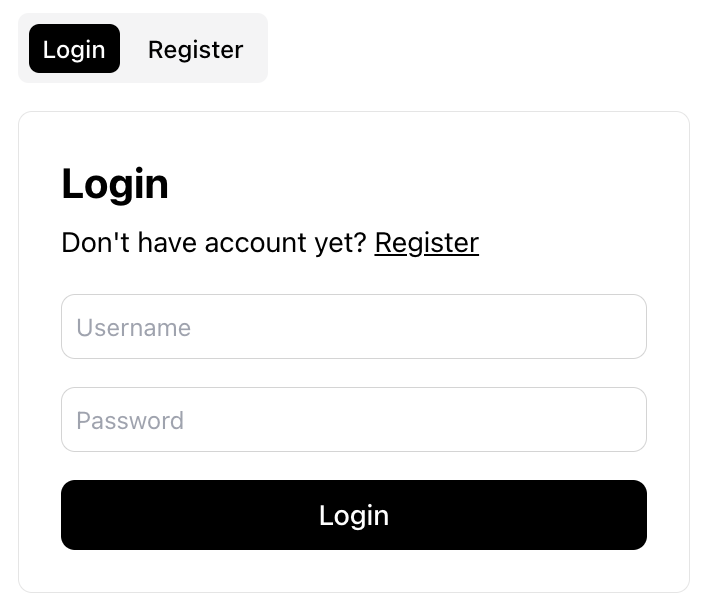
\includegraphics[width=7cm]{images/tabs}
  \captionsetup{justification=centering,margin=2cm}
  \caption{tabs} \label{picture:tabs}
\end{figure}

\subsection{Textarea}
Textarea je vstupní komponenta, která umožňuje uživatelům zadat víceřádkový text. Používá se v formulářích, kde je potřeba více místa pro text, například v komentářích, poznámkách nebo popisech.

\begin{figure}[H]
  \centering
  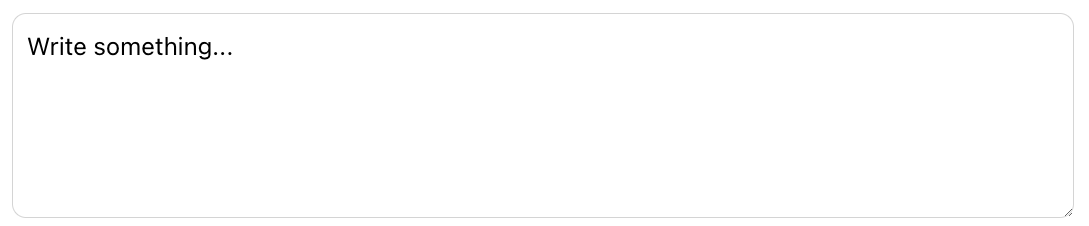
\includegraphics[width=10cm]{images/textarea}
  \captionsetup{justification=centering,margin=2cm}
  \caption{textarea} \label{picture:textarea}
\end{figure}

\subsection{Text input}
Text input je základní vstupní pole, které umožňuje uživatelům zadávat text. Používá se v formulářích pro zadání jednoduchých textových informací, jako jsou jména, e-maily nebo hesla. Text input může mít různé typy, například text, email, password nebo number.

\begin{figure}[H]
  \centering
  
\includegraphics[width=10cm]{images/textinput}
  \captionsetup{justification=centering,margin=2cm}
  \caption{textinput} \label{picture:textinput}
\end{figure}

\subsection{Tooltip}
Tooltip je komponenta, která poskytuje dodatečné informace o prvku, když na něj uživatel najede myší nebo se na něj jiným způsobem zaměří. Tooltipy se používají ke zlepšení uživatelského zážitku tím, že poskytují kontext nebo vysvětlení bez nutnosti zabírat místo na obrazovce.

\begin{figure}[H]
  \centering
  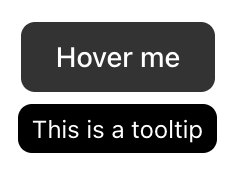
\includegraphics[width=3cm]{images/tooltip}
  \captionsetup{justification=centering,margin=2cm}
  \caption{tooltip} \label{picture:tooltip}
\end{figure}

\clearpage

\section{Bloky}
Bloky jsou větší, komplexní komponenty, které fungují jako samostatné sekce webových aplikací. Dělí se na dva typy a to sice pro jedno použití a znovupoužitelné. Mezi komponenty pro jedno použití patří např. úvodní stránka. Tyto bloky většinou obsahují statický obsah, který se nemění a je na vývojářích, aby textace a obsah doplnili dle potřeby. Naopak znovupoužitelné bloky jsou komponenty, které se mohou použít na více místech aplikace. Mezi ně patří např. sekce, které se mohou nacházet na jedné stránce několikrát. \footnote{Tento nápad byl přidán během tvorby této práce i do knihovny shadcn/ui. Vzhledem k přidání do této úspěšné knihovny se potrzuje, že tato myšlenka je správná a má smysl.}

Bloky značně zlepšují efektivitu vývoje tím, že standardizují často používané UI prvky do předdefinovaných šablon. Díky tomu mohou vývojáři snadno implementovat a opakovaně používat komplexní UI struktury bez nutnosti opětovného kódování nebo redesignu těchto částí pro každý nový projekt.

Hlavní přínosy bloků spočívají v jejich schopnosti snižovat redundantní kód a zvyšovat znovupoužitelnost komponent napříč projekty. Díky konzistentní implementaci jednotlivých bloků mohou vývojáři efektivně reagovat na nové požadavky nebo změny v designu bez rozsáhlých úprav celé aplikace.

\begin{figure}[H]
  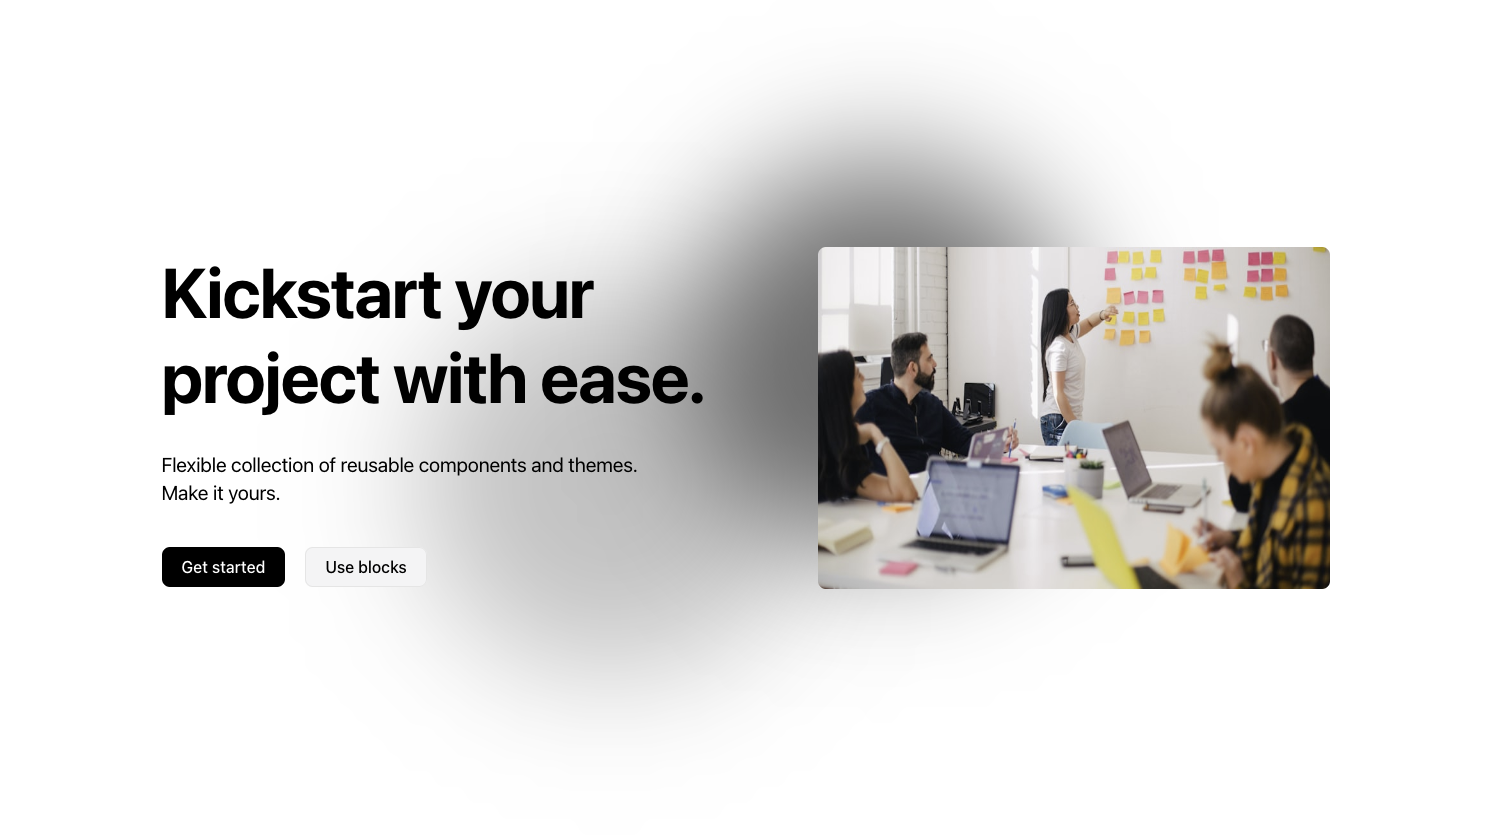
\includegraphics[width=\textwidth]{images/hero-block}
  \caption{Blok na úvodní stránku} \label{picture:hero-block}
\end{figure}

\subsection{Hero}

Hero sekce je úvodní část stránky, která zaujme návštěvníky a poskytuje hlavní informace nebo klíčové sdělení. Obvykle se nachází v horní části stránky a obsahuje poutavý obrázek nebo video, výrazný nadpis a krátký popis. Je navržena tak, aby upoutala pozornost uživatelů a povzbudila je k dalšímu prozkoumání webu nebo provedení určité akce, například kliknutí na tlačítko s výzvou k akci (CTA).

\subsection{Section}

Section je univerzální blok, který rozděluje obsah stránky do logických částí. Každá sekce může mít vlastní obsah, jako jsou texty, obrázky nebo interaktivní prvky, a slouží k organizaci informací na stránce tak, aby byly přehledné a snadno čitelné. Sekce pomáhají strukturovat stránku a usnadňují uživatelům orientaci a nalezení relevantních informací.

\subsection{Features}

Features blok slouží k prezentaci hlavních funkcí nebo výhod produktu či služby. Obvykle se skládá z řady ikon nebo obrázků doplněných krátkými popisy, které stručně a jasně vysvětlují, co produkt nebo služba nabízí. Tento blok pomáhá uživatelům rychle pochopit, jaké benefity mohou očekávat, a usnadňuje rozhodování o koupi nebo dalším využití.

\subsection{References}

References blok je určen k zobrazení referencí, recenzí nebo citací od spokojených zákazníků či partnerů. Tento blok zvyšuje důvěryhodnost a kredibilitu produktu nebo služby tím, že poskytuje sociální důkazy o jeho kvalitě a spolehlivosti. Obsahuje často fotografie, jména a krátké výpovědi od skutečných uživatelů, což pomáhá budovat důvěru u potenciálních zákazníků.

\subsection{Contact}

Contact blok slouží k zobrazení kontaktních informací a formulářů, které umožňují uživatelům snadno se spojit s provozovatelem webu nebo podpůrným týmem. Tento blok obvykle obsahuje informace jako jméno, telefonní číslo a e-mailová adresa. Může také obsahovat kontaktní formulář, který uživatelům umožňuje rychle zaslat zprávu nebo dotaz přímo z webové stránky.

\subsection{Auth}

Auth blok se používá pro autentizaci uživatelů, tedy pro přihlášení, registraci nebo obnovení hesla. Obsahuje formuláře, které uživatelům umožňují zadávat své přihlašovací údaje, vytvářet nové účty nebo obnovit zapomenuté heslo. Tento blok je navržen pro webové aplikace, které vyžadují bezpečný přístup k uživatelským účtům a osobním informacím.

\subsection{Blog}

Blog blok slouží k zobrazení seznamu článků nebo příspěvků na blogu. Tento blok obvykle obsahuje náhledy článků s titulky, krátkými úryvky a odkazy na celé články. Blog sekce pomáhá udržovat web aktuální a informativní, zlepšuje SEO a poskytuje uživatelům hodnotný obsah, který je může zaujmout a přivést zpět na web.

\subsection{Header}

Header je horní část webové stránky, která obvykle obsahuje logo, navigační menu a další prvky, jako jsou odkazy na přihlášení, nákupní košík nebo vyhledávací pole. Header je důležitým prvkem každé webové stránky, protože poskytuje uživatelům rychlý přístup k hlavním sekcím webu a usnadňuje navigaci. Důraz na jednoduchost a přehlednost v headeru zlepšuje uživatelskou zkušenost a orientaci.

\section{CLI}
Pro usnadnění práce s UI knihovnou je potřeba vyvinout CLI, které pomůže s inicializací a přidávání komponent do projektů.

\subsection{Inicializace}
Inicializace knihovny prostřednictvím CLI zajišťuje, že jsou přidány všechny závislosti a další potřebné soubory jsou připraveny k použití ihned po vytvoření nového projektu. Příkaz pro inicializaci může vypadat například takto \mintinline{console}|npx @v-moravec/ui init|. V rámci tohoto příkazu je potřeba zkontrolovat, zda již soubory neexistují. Pokud by existovaly, měl by uživatel dostat možnost zvolit, zda chce přepsat stávající soubory nebo pokračovat bez změn. V případě chybějících souborů se automaticky vytvoří nové.

Získání souborů a závislotí by mělo být automatizováno, aby se zabránilo chybám a zjednodušil se vývoj knihovny. Nejjednodušší způsob je soubory vytáhnout do API dokumentace, odkud je možné s nimi pracovat na úrovní CLI. Pro tuto automatizaci je možné využít vlastních Nuxt modulů. Jako inspiraci lze použít modul, který využívá knihovna NuxtUI. \cite{NuxtUISourceCodeModule}

\subsection{Přidání komponent}
Přidání komponent a bloků využije stejného principu jako inicializace projektu. Příkaz pro přidání komponenty může vypadat například takto:\\

\mintinline{console}|npx @v-moravec/ui add [...componentName/blockName]|\\

Při přidání komponenty je potřeba zkontrolovat, zda již soubory neexistují. Pokud by existovaly, měl by uživatel dostat možnost zvolit, zda chce přepsat stávající soubory nebo pokračovat bez změn. V případě chybějících souborů se automaticky vytvoří nové.

Z hlediska zdrojového kódu komponent a bloků bude potřeba více modulů, které na API vystaví všechny potřebné informace. Také bude potřeba v rámci každého souboru zjistit jeho závislosti a to na externích knihovnách, komponentách v rámci knihovny a dalších souborech, jako například composables. Toho je možné dosáhnout pomocí pattern matchingu.

\subsection{Publikace balíčku}
Jak bylo popsáno v sekci o technologiích, pro správu verzí balíčku se používá nástroj Changesets. Workflow pak vypadá následovně:

\begin{enumerate}
  \item Vytvoření změn v kódu.
  \item Vytvoření nové verze pomocí Changeset.
  \item Nahrání změn na GitHub.
  \item Spuštění GitHub Actions workflow pro publikaci balíčku.
  \item Publikace nové verze balíčku.
\end{enumerate}

Díky této automatizaci je možné rychle a bezpečně publikovat nové verze balíčku, aniž by bylo nutné manuálně upravovat potřebné soubory.

\section{Závěr}
V této kapitole byly popsány kroky a procesy vedoucí k navržení sbírky znovupoužitelných Nuxt komponent. Byly identifikovány a zdokumentovány prvky, které ovlivňují design a implementaci UI komponent.

Hlavním cílem navrhované sbírky komponent je vytvoření robustního základu, který umožní efektivní vývoj webových aplikací s využitím moderních frontend technologií. Tento návrh reflektuje nejnovější trendy ve vývoji webových aplikací a také přináší řadu nástrojů, které podporují celý životní cyklus vývoje od návrhu po nasazení a údržbu.

V další kapitole Implementace se práce zaměří na vytvoření navržených komponent. Diskutovány budou také výzvy a řešení, která byla během implementace identifikována.



%! Author = Vojta
%! Date = 21.1.2024

\chapter{Implementace}\label{ch:implementation}

\section{Úvod}
V této kapitole bude zaměřena pozornost na implementaci sbírky znovupoužitelných Nuxt komponent. Implementace je fází vývoje, kde jsou teoretické návrhy a plánování transformovány do praktických a funkčních výsledků. Tato fáze zahrnuje konkrétní kroky a postupy potřebné k vytvoření komponent, dokumentace a CLI, které splňují stanovené požadavky a cíle.

Cílem této kapitoly je podrobně popsat strukturu projektu, jednotlivé části implementace a jejich vzájemné propojení. Dále bude věnována pozornost dokumentaci komponent, jejich kódu a blokům, které tvoří základ pro uživatelsky přívětivé a efektivní rozhraní. Implementace také zahrnuje tvorbu a použití příkazového řádku (CLI), který usnadňuje práci s komponentami a jejich integraci do různých projektů.

\section{Struktura projektu}
Pro zajištění efektivní správy a rozvoje projektu byla použita struktura monorepozitáře. Monorepozitář umožňuje uchovávat kód pro více balíčků v jednom repozitáři, což usnadňuje správu závislostí a zajišťuje konzistenci napříč celým projektem.

\subsection{Struktura monorepozitáře}
Struktura monorepozitáře je vidět na výpisu kódu \ref{lst:monorepo-structure}.

\begin{listing}[h]
\caption{Struktura monorepozitáře}
\label{lst:monorepo-structure}
\begin{code}[bash]
/v-moravec-ui
|-- /packages
|   |-- /cli
|   |   |-- /src
|   |   |   |-- /commands
|   |   |   |   |-- /add.ts
|   |   |   |   |-- /init.ts
|   |   |   |-- /utils
|   |   |   |   |-- /getPackageManager.ts
|   |   |   |   |-- /handleError.ts
|   |   |   |   |-- /checkNuxtProject.ts
|   |   |   |   |-- /installDependencies.ts
|   |   |   |   |-- /removeDuplicates.ts
|   |   |   |-- constants.ts
|   |   |   |-- index.ts
|-- /apps
|   |-- /docs
|   |   |-- /components
|   |   |   |-- /ui
|   |   |   |-- /block
|-- package.json
|-- pnpm-workspace.yaml
\end{code}
\end{listing}

\subsection{Popis jednotlivých částí}

\begin{itemize}
    \item /packages: Tento adresář obsahuje jednotlivé balíčky, které jsou součástí monorepozitáře.
    \item /cli: Tento balíček obsahuje CLI nástroje pro správu projektu. V adresáři src/commands se nachází jednotlivé příkazy jako add.ts a init.ts. V adresáři src/utils jsou různé užitečné funkce. Další soubory zahrnují constants.ts a index.ts, které obsahují základní konfiguraci a vstupní bod CLI nástroje.
    \item /apps: Tento adresář obsahuje jednotlivé aplikace. V tomto případě se jedná pouze o dokumentační aplikaci. V budoucnu mohou být přidány další aplikace, jako je například ukázková aplikace využívající komponenty.
    \item /docs: Dokumentační aplikace, která demonstruje použití vytvořených komponent a bloků. V adresáři components se nachází další podadresáře jako ui a block.
    \item /ui: Zde jsou umístěny všechny základní komponenty, které jsou součástí sbírky.
    \item /block: Zde jsou umístěny bloky, které kombinují jednotlivé komponenty do složitějších struktur.
    \item package.json: Hlavní soubor pro správu závislostí a skriptů na úrovni celého monorepozitáře.
    \item pnpm-workspace.yaml: Konfigurační soubor pro pnpm, který definuje strukturu workspace a zahrnuje všechny balíčky a aplikace.
\end{itemize}

Díky této struktuře je možné jednoduše vyvíjet komponenty, jejich dokumentaci a CLI bez nutnosti spravovat více repozitářů a závislostí.

\section{Dokumentace}
Implementace začala vytvořením nového projektu pomocí příkazu, který inicializuje projekt s připraveným Nuxt Content modulem.\\

\mintinline{console}|npx nuxi@latest init v-moravec-ui -t content|\\

Tento příkaz vytvoří základní strukturu projektu a přidá potřebné závislosti, což umožňuje rychlý start vývoje. Po vytvoření projektu byly přidány další moduly nezbytné pro vývoj, jako je Tailwind CSS, Nuxt Icon, Nuxt Color Mode a Nuxt SEO. Tyto moduly poskytují širokou škálu funkcí pro stylování, správu ikon, podporu tmavého režimu a optimalizaci SEO.

Aby bylo možné využít komponenty v rámci dokumentace, bylo potřeba je označit jako globální v souboru \emph{nuxt.config.ts}. V rámci dokumentace je to dobré řešení pro minimalizaci duplikace kódu a zjednodušení práce s komponentami, ale pro koncové aplikace není nutné toto nastavení přidávat. Ukázka kódu \ref{lst:global-components} zobrazuje, jak lze označit komponenty jako globální.

\begin{listing}[h]
    \caption{Označení komponent jako globální}
    \label{lst:global-components}
    \begin{code}
components: {
  dirs: [
    {
      path: '~/components/ui',
      global: true,
      prefix: 'Ui',
    },
    '~/components',
  ],
},
\end{code}
\end{listing}

Nastavení Tailwind CSS vyžadovalo specifikaci složek, které má při \emph{buildu} procházet a hledat styly, aby byly zahrnuty pouze potřebné styly díky využití \emph{tree shakingu}. Toto nastavení bylo přidáno do souboru tailwind.config.ts. \emph{Tree shaking} umožňuje minimalizaci velikosti výsledného balíčku tím, že odstraní nepoužívané styly, což zlepšuje výkon aplikace. Ukázka kódu \ref{lst:tailwind-config} ukazuje, jak lze nastavit Tailwind CSS na procházení složek se zdrojovým kódem. Kromě toho je zde zobrazena i struktura, která se používá pro definování barev, velikostí a dalších vlastností.

\begin{listing}[h]
    \caption{Konfigurační soubor pro Tailwind}
    \label{lst:tailwind-config}
    \begin{code}
import type { Config } from 'tailwindcss'
import typography from '@tailwindcss/typography'
import containerQueries from '@tailwindcss/container-queries'

export default <Partial<Config>>{
    darkMode: 'class',
    content: ['components/**/*.{vue,ts}', 'layouts/**/*.vue', 'pages/**/*.vue'],
    theme: {
        extend: {
            colors: {
                background: 'hsl(var(--background))',
                primary: {
                    DEFAULT: 'hsl(var(--primary))',
                    contrast: 'hsl(var(--primary-contrast))',
                },
                secondary: {
                    DEFAULT: 'hsl(var(--secondary))',
                    contrast: 'hsl(var(--secondary-contrast))',
                },
                disabled: {
                    DEFAULT: 'hsl(var(--disabled))',
                    contrast: 'hsl(var(--disabled-contrast))',
                },
                border: 'hsl(var(--border))',
            },
            borderRadius: {
                sm: 'calc(var(--radius) - 4px)',
                md: 'calc(var(--radius) - 2px)',
                lg: 'var(--radius)',
                xl: 'calc(var(--radius) + 4px)',
                '2xl': 'calc(var(--radius) + 8px)',
                '3xl': 'calc(var(--radius) + 16px)',
            },
        },
    },
    plugins: [typography, containerQueries],
}
\end{code}
\end{listing}

\section{Komponenty}
Jedna ze zajímavějších věcí, kterou bylo potřeba vyřešit, je, jak psát znovupoužitelné komponenty. Je možné používat \emph{sloty}, které mají jména, případně použít \emph{wrappery} neboli obaly, které zachovávají logiku v sobě. V rámci konkurenčních řešení se často používají \emph{wrappery}, ačkoliv to je pravděpodobně způsobeno tím, že se jedná o řešení pro React, potažmo o řešení převzaté z původní React verze. Ve Vue je jednodušší řešení přímo pomocí pojmenovaných \emph{slotů} - poté se kód zjednodušší a nemusí se používat direktivy jako \emph{provide} a \emph{inject}, které zhoršují čitelnost kódu.

Pojmenované \emph{sloty} jsou užitečné pro složitější komponenty, které vyžadují více oblastí pro různé části obsahu. Pojmenované \emph{sloty} se definují pomocí atributu name na <slot> značce a obsah se vkládá pomocí template tagu s atributem v-slot.

\begin{listing}[h]
    \caption{Pojmenované sloty - definice}
    \label{lst:named-slots}
    \begin{code}[jsx]
<!-- Card.vue -->
<template>
  <div class="card">
    <header>
      <slot name="header"></slot>
    </header>
    <main>
      <slot></slot>
    </main>
    <footer>
      <slot name="footer"></slot>
    </footer>
  </div>
</template>
\end{code}
\end{listing}

\begin{listing}[h]
    \caption{Pojmenované sloty - použití}
    \label{lst:named-slots-usage}
    \begin{code}[html]
<!-- ParentComponent.vue -->
<template>
    <Card>
    <template #header>
        <h1>Card Header</h1>
    </template>
    <p>This is the main content.</p>
    <template #footer>
        <p>Card Footer</p>
    </template>
    </Card>
</template>
\end{code}
\end{listing}

\clearpage

\subsection{Použité závislosti}

\subsubsection{Nuxt Icon}
Tvorba vlastních ikon je časově náročná a může být složitá. Ideální je využít již hotové ikony, které jsou k dispozici na internetu. Je více možností, jak toho dosáhnout, například lze kopírovat SVG kód a uložit jej do assetů nebo třeba do Vue komponent. To může být ale neefektivní a nepřehledné. Pro použití ikon z online zdrojů existuje modul Nuxt Icon, který zpřístupňuje mnoho ikon pro efektivní použití v aplikacích. Tento modul je velmi pokročilý, a proto je v dokumentaci doporučené jej použít. Do budoucna je možné přidat obal, aby se zachovalo konzistentní pojmenování komponent.

\subsubsection{Floating UI}
Plovoucí prvky nejsou triviální na implementaci. Je potřeba zajistit, aby byly viditelné vždy, když je uživatel potřebuje. Pro tento účel byla použita knihovna Floating UI, která poskytuje jednoduché rozhraní pro vytváření plovoucích prvků. Tato knihovna je velmi užitečná pro vytváření interaktivních prvků, jako jsou tlačítka, odkazy a formuláře. Byl vytvořen jednoduchý \emph{wrapper} formou \emph{composable}. Díky této \emph{composable} je možné vytvářet plouvoucí prvky v komponentách pomocí jednoho řádku s parametry.

\begin{listing}[H]
    \caption{Composable obalující Floating UI}
    \label{lst:floating-ui}
    \begin{code}
import type { Placement, Strategy, MaybeElement } from '@floating-ui/vue'
import { useFloating, autoUpdate, offset, flip, shift } from '@floating-ui/vue'

export const useUiFloating = ({
  placement = 'bottom',
  offsetSize = 5,
  strategy = 'fixed',
}: Partial<{
  placement: Placement
  offsetSize: number
  strategy: Strategy
}>) => {
  const anchor = ref<MaybeElement<HTMLElement>>(null)
  const floating = ref<MaybeElement<HTMLElement>>(null)

  const { floatingStyles } = useFloating(anchor, floating, {
    strategy,
    placement,
    whileElementsMounted: autoUpdate,
    middleware: [shift(), flip({ fallbackAxisSideDirection: 'end' }), offset(offsetSize)],
  })

  return { anchor, floating, floatingStyles } as const
}
\end{code}
\end{listing}

\begin{listing}[H]
    \caption{Použití composable v komponentě}
    \label{lst:floating-ui-usage}
    \begin{code}
const { anchor, floating, floatingStyles } = useUiFloating({ placement: props.placement, offsetSize: props.offsetSize })
\end{code}
\end{listing}

V budoucnu je možné, že nebude potřeba používat žádné knihovny díky nativní implementaci přímo v prohlížečích. Všechny moderní prohlížeče toto nové API podporují, avšak pro lepší podporu starších browserů je lepší použití výše zmíněné knihovny. \cite{PopoverAPI}

\subsubsection{Embla Carousel}
Jedna z dalších komponent, která je složitá na implementaci, je \emph{carousel}. Pro tento účel byla použita knihovna Embla Carousel. Byl vytvořen \emph{wrapper} nad jejím API v rámci několika komponent, které je možné dodatečně stylovat a ovlivňovat jejich chování.

\subsubsection{Headless UI}
Jak bylo popsáno v dřívějších kapitolách, pro implementaci některých prvků byla použita knihovna Headless UI. Více informací o této knihovně je v kapitolách Analýza a Technologie.

\clearpage

\section{Kód komponent a bloků}
Bylo potřeba vymyslet, jak zobrazit kód bez jeho duplikace. V tom pomohl zdrojový kód knihovny Nuxt UI. Tato knihovna využívá principu vygenerování \emph{endpointů} pro zobrazení zdrojového kódu přímo ze souborů s komponentami, popřípadě ze souborů s ukázkami použití. \cite{NuxtUISourceCodeModule}

Pomocí několika modulů, které byly vytvořeny pro tento účel, bylo možné poskytnout kód komponent, bloků a dalších pomocných souborů na API aplikace, která obsahuje dokumentaci. Díky tomuto způsobu je možné kód zobrazit v dokumentaci a také použít v rámci CLI pro přidání komponent do projektu.

V první části bylo potřeba získat informace o komponentách a blocích. To bylo dosaženo pomocí \emph{hooku}, který poskytuje seznam všech komponent a bloků. Tento seznam byl filtrován podle určitých kritérií a následně byl uložen do proměnné. Ukázka kódu \ref{lst:module} ukazuje, jak byl získán seznam komponent a bloků.

\begin{listing}[H]
    \caption{Prvotní získání informací o komponentách}
    \label{lst:module}
    \begin{code}
nuxt.hook('components:extend', async (_components) => {
    components = _components
        .filter(
        (v) =>
            v.shortPath.includes('components/content/examples/') ||
            v.shortPath.includes('components/block/') ||
            v.shortPath.includes('components/ui/') ||
            v.shortPath.includes('components/content/blocks/')
        )
        .reduce((acc, component) => {
        acc[component.pascalName] = component
        return acc
        }, {})
    await stubOutput()
})
\end{code}
\end{listing}

Také bylo využito dalšího \emph{hooku} \mintinline{javascript}|nuxt.hook('vite:extend', (vite: any) => {})|, který umožňuje při startu \emph{buildu} volat funkci, ve které se všechny komponenty zpracují a přidají do proměnné. Konkrétně se volá funkce \mintinline{javascript}|await fetchComponents()|. V rámci této funkce se získané komponenty transformují do chtěné podoby. Následující ukázka vynechává kontroly dat, které nejsou nijak zajímavé a ukazuje pouze základní transformaci dat.

\clearpage

\begin{listing}[H]
    \caption{Transformace dat komponent}
    \label{lst:module}
    \begin{code}
const code = await fsp.readFile(component.shortPath, 'utf-8')

components[component.pascalName] = {
    code,
    shortPath: component.shortPath,
    pascalName: component.pascalName,
}
\end{code}
\end{listing}

Poté se obsah proměnné uloží do souboru a jeho obsah se vrací v rámci \emph{endpointu} API. Je nutné přidat \emph{endpoint} do souboru \emph{server/api/component-list.get.ts}, který obsahuje logiku pro získání dat. Jak se soubory spojí, je ukázáno v příloze \ref{lst:link-to-endpoint}, obsah samotného \emph{endpointu} v ukázce \ref{lst:code-example-endpoint}.

Ještě jedna důležitá část, která se v rámci ukázek kódu neřeší, jsou různé závislosti na balíčky, další komponenty a podpůrné soubory jako \emph{composables}. Aby bylo možné zjednodušit proces instalace nových komponent, bylo potřeba přidat tato data. Proto vznikly další moduly pro komponenty, bloky a \emph{composables}. Transformace dat je zobrazena v ukázce \ref{lst:cli-data-transform}.

Pro zobrazení kódu má Nuxt Content zabudovanou funkci. \cite{NuxtContentCodeHighlighting} Avšak bylo potřeba si vytvořit ještě vlastní komponentu, která bude zobrazovat kód získaný z API, protože zvýraznění kódu je nativně podporované pouze v Markdown souborech. Tato komponenta využívá Shiki \emph{highlighteru}, tedy stejný princip, jaký používá Nuxt Content. Ukázka kódu \ref{lst:code-highlighter} ukazuje, jak je možné vytvořit komponentu pro zobrazení kódu.

\section{CLI}
Vytvoření příkazu, který CLI umožňuje použít, vypadá následovně:

\begin{listing}[H]
    \caption{Příkaz pro přidání komponent a bloků}
    \label{lst:cli-install}
    \begin{code}
export const add = new Command()
.name('add')
.description('add components and blocks to your application')
.argument('[componentsAndBlocks...]', 'components and blocks to add')
.action(async (componentsAndBlocks, opts) => {
    // Logika pro přidání komponent a bloků
})        
\end{code}
\end{listing}

\clearpage

Pro kontrolu, zda jsou všechna data z API v pořádku, byl použit Zod. Zde je ukázka vytvoření schématu a použití pro validaci dat:

\begin{listing}[H]
    \caption{Validace dat pomocí Zod}
    \label{lst:cli-install}
    \begin{code}
const componentAndBlockSchema = z.object({
  code: z.string(),
  uiDependencies: z.string().array().optional(),
  dependencies: z.string().array().optional(),
  composableDependencies: z.string().array().optional(),
  shortPath: z.string(),
  pascalName: z.string(),
})

const componentsAndBlocksSchema = z.record(z.string(), z.array(componentAndBlockSchema))

const components = componentsAndBlocksSchema.safeParse(await (await fetch(BASE_URL + '/component-list')).json())
const blocks = componentsAndBlocksSchema.safeParse(await (await fetch(BASE_URL + '/block-list')).json())

if (!components.success) {
    return handleError(components.error)
}
if (!blocks.success) {
    return handleError(blocks.error)
}

// Pokračování práce s daty
\end{code}
\end{listing}

\section{Závěr}
V této kapitole byla podrobně popsána implementace sbírky znovupoužitelných Nuxt komponent. Byly popsány jednotlivé části projektu, jejich struktura a vzájemné propojení, čímž byl vytvořen komplexní nástroj pro vývoj a použití této kolekce. Dokumentace komponent byla zpracována tak, aby usnadnila jejich používání, což zajišťuje jejich efektivní integraci do různých projektů. Velká pozornost byla věnována nejen samotnému kódu komponent, ale také tvorbě pomocných nástrojů.
%! Author = Vojta
%! Date = 25.11.2021

\chapter{Testování}

\subsection{Body pro testování}
\begin{itemize}
    \item Uživatelské testování
\end{itemize}


%! Author = Vojta
%! Date = 21.1.2024

\chapter{Možnosti rozšíření}

V této kapitole se zaměříme na možnosti rozšíření sbírky znovupoužitelných Nuxt komponent. Po úspěšné implementaci základní sady komponent je důležité zvážit, jakým způsobem lze tuto sbírku dále rozšiřovat a přizpůsobovat novým požadavkům.

Budou zde prozkoumány možnosti přidávání nových komponent, bloků a funkcionalit, které mohou zvýšit hodnotu a využitelnost celé sbírky. Dále se bude diskutovat o integraci dalších nástrojů a technologií, které mohou usnadnit vývoj a zlepšit uživatelskou zkušenost.

Cílem této kapitoly je poskytnout ucelený pohled na možnosti rozšíření a ukázat, jak lze existující sbírku komponent nadále zdokonalovat a přizpůsobovat novým výzvám a příležitostem.

\section{Přidání komponent a bloků}
Aktuální kolekce komponent zahrnuje základní sadu komponent, které byly navrženy tak, aby pokrývaly širokou škálu běžných požadavků ve webových aplikacích. Testování ukázalo, že tyto komponenty jsou přehledné, snadno použitelné a poskytují dobrý základ pro rychlé vytvoření webových stránek. Nicméně existuje prostor pro rozšíření sbírky o další komponenty a bloky, které mohou poskytnout uživatelům větší flexibilitu a možnosti přizpůsobení.

\subsection{Přidání bloků}
Rozšíření sbírky o více bloků a jejich verzí umožňuje uživatelům přizpůsobit si aplikace s větší flexibilitou a znovupoužitelností. Bloky mohou být navrženy tak, aby pokrývaly širokou škálu běžných i specifických případů, od navigačních prvků po složité sekce. Zde je výpis několika bloků, které by mohly být přidány do sbírky:

\begin{description}
  \item[Pricing] Blok pro zobrazení cenových plánů nebo balíčků.
  \item[Sponzoři/Partneři] Sekce, která zobrazuje loga sponzorů nebo partnerů.
  \item[FAQ sekce] Sekce s často kladenými otázkami.
  \item[Error stránky] Stránky pro zobrazení chybových stavů.
  \item[About sekce] Tato sekce je často velmi specifická pro dané téma stránek. Avšak nějaké obecné koncepty mohou být zahrnuty.
  \item[Interaktivnější bloky] Pro složitější aplikace jako jsou eshopy nebo platformy pro správu obsahu je potřeba přidat další bloky. Jako příklad takového bloku může být stránka produktu nebo třeba košík.
\end{description}

\subsection{Přidání komponent}
Dodatek nových komponent do knihovny by měl reflektovat aktuální trendy ve webovém designu, zatímco zároveň by měl pokrývat nové požadavky uživatelů. Například integrace komponent pro pokročilé uživatelské interakce.

\begin{description}
  \item[Calendar] Komponenta pro různá zobrazení kalendáře.
  \item[Command pallete] Komponenta pro rychlé vyhledávání a spouštění akcí.
  \item[Date picker] Komponenta pro výběr data.
  \item[Skeleton] Komponenta pro zobrazení načítání obsahu.
  \item[Slider] Komponenta pro výběr hodnoty nebo intervalu.
\end{description}

\section{Přidání ukázkových stránek/aplikací}
Vytvoření sad ukázkových stránek nebo aplikací využívajících komponent poskytuje uživatelům možnost rychlejšího vývoje. Tyto stránky mohou zahrnovat různé scénáře použití od jednoduchých landing stránek po složitější platformy.

\section{Přidání možností konfigurace}
Umožnění uživatelům konfigurovat komponenty pomocí vlastního konfiguračního souboru nabízí vyšší úroveň personalizace a kontrolu. Uživatelé již nyní mohou definovat globální nastavení, jako jsou motivy, typografie a barvy, které budou automaticky aplikovány na všechny komponenty. Nicméně někteří uživatelé mohou chtít konfigurovat např. umístění komponent a bloků a jejich prefix. Prozatím pro konzisteci napříč projekty není možné tyto nastavení měnit, avšak v budoucnu je možné přehodnotit tuto možnost.

\section{Figma Kit}
Momentálně je Figma Kit spíše statický, jeho aktualizace o responzivní design a interaktivní prvky umožní designérům a vývojářům lepší spolupráci a rychlejší iteraci designů. Tato rozšíření mohou zahrnovat varianty komponent pro různé obrazovky a zařízení, interaktivní stavy pro hover a kliknutí, a integrované prototypování funkcí. Poskytnutí těchto nástrojů v Figma kitu umožní týmům efektivně testovat a upravovat UI/UX designy před jejich implementací.

\section{Testy komponent}
Automatizované testování může být zajímavé rozšíření pro zajištění kvality a udržitelnosti knihovny komponent. Použití robustního testovacího \emph{frameworku}, který umožňuje jak jednotkové testy, tak integrační a end-to-end testy, značně zvyšuje spolehlivost a snižuje pravděpodobnost chyb při budoucích aktualizacích komponent. Použití nástrojů jako \emph{@nuxt/test-utils} nebo Cypress poskytuje komplexní pokrytí testů a integrovanou podporu pro simulaci uživatelských interakcí a asertace stavu UI. Navrhnout testovací scénáře, které mapují běžné a okrajové případy užití komponent, zvyšuje důvěru v kód a usnadňuje kontinuální integraci a nasazení. Na druhou stranu je otázka, jak tyto testy integrovat do koncových aplikací a zda je to vůbec možné.

\section{Vytváření stylů}
Vývoj \uv{Theme Creator} nástroje, který bude integrován přímo do dokumentace, umožní uživatelům v reálném čase vizualizovat a upravovat vzhled komponent. Tento nástroj by měl nabídnout intuitivní rozhraní pro výběr barev, fontů, zaoblení hran a dalších stylistických prvků. Takový nástroj značně usnadní proces designu a vývoje tím, že poskytne okamžitou zpětnou vazbu na změny provedené v tématu a umožní uživatelům exportovat výsledné styly pro použití ve svých projektech.

%! Author = Vojta
%! Date = 21.1.2024

\chapter{Závěr}

Cílem této diplomové práce bylo analyzovat současný stav UI knihoven a na základě toho navrhnout a implementovat vlastní řešení. V průběhu práce se podařilo vytvořit komplexní ekosystém, který zahrnuje několik důležitých součástí.

Mezi hlavní části tohoto ekosystému patří:

\begin{description}
  \item[Dokumentace] Dokumentace je dostupná online na adrese \url{https://ui.vojtamoravec.cz}, což umožňuje snadnou dostupnost a aktualizaci informací pro uživatele knihovny.
  \item[Knihovna komponent ve Figmě] Na adrese \url{https://www.figma.com/community/file/1331024596435699926/v-moravec-ui} se nachází knihovna komponent, která je navržena tak, aby usnadnila designérům a vývojářům spolupráci a integraci návrhů do kódu.
  \item[CLI nástroj] Pomáhá s instalací a správou komponent v rámci projektu.
\end{description}

V průběhu práce byly identifikovány a dokumentovány prvky, které ovlivňují design a implementaci komponent a samotné dokumentace. Byly popsány kroky vedoucí k navržení sbírky znovupoužitelných Nuxt komponent, které reflektují nejnovější trendy ve vývoji webových aplikací. Návrh a implementace zahrnovaly moderní frontend technologie a nástroje, které podporují celý životní cyklus vývoje od návrhu po nasazení a údržbu.

Testování provedené v rámci této práce odhalilo jak silné stránky, tak oblasti pro zlepšení kolekce komponent. Dokumentace byla obecně hodnocena kladně, ale bylo také jasné, že existuje prostor pro její zlepšení, zejména v ukázkách možností komponent. Jednoduchá rozšiřitelnost a flexibilita komponent byly hodnoceny jako důležité prvky kolekce, které umožňují snadnou integraci a rychlý vývoj webových stránek.

V závěru je třeba zdůraznit, že práce na této komponentové knihovně není ukončena. Plánují se další vylepšení a rozšíření, aby byla zajištěna jeho dlouhodobá udržitelnost a užitečnost pro vývojáře. Budoucí rozšíření zahrnují přidání nových bloků, komponent, ukázkových stránek a aplikací, možnosti konfigurace, Figma Kitu a testování komponent, což vše přispěje ke zlepšení kvality a uživatelského zážitku.

Tato diplomová práce tak poskytuje pevný základ pro další vývoj a rozšiřování komponentové knihovny, která bude sloužit jako užitečný nástroj pro vývojáře při vytváření moderních webových aplikací.


% % Do not forget to include Introduction
%---------------------------------------------------------------
\chapter{Ut enim ad minim veniam}
%---------------------------------------------------------------
\setcounter{page}{1}

\begin{chapterabstract}
	\lipsum[1]
\end{chapterabstract}

\lipsum[2][1-4]{} [1]

\lipsum[4]

%---------------------------------------------------------------
\section{Ut enim ad minim veniam}
%---------------------------------------------------------------

\lipsum[6-7]

\begin{figure}
\centering
%\includegraphics[scale=0.4]{pic/index}
\resizebox{\textwidth}{!}{
\begin{tikzpicture}[level/.style={sibling distance=60mm/#1}]
\node [circle,draw] (z){$n$}
  child {node [circle,draw] (a) {$\frac{n}{2}$}
    child {node [circle,draw] (b) {$\frac{n}{2^2}$}
      child {node {$\vdots$}
        child {node [circle,draw] (d) {$\frac{n}{2^k}$}}
        child {node [circle,draw] (e) {$\frac{n}{2^k}$}}
      }
      child {node {$\vdots$}}
    }
    child {node [circle,draw] (g) {$\frac{n}{2^2}$}
      child {node {$\vdots$}}
      child {node {$\vdots$}}
    }
  }
  child {node [circle,draw] (j) {$\frac{n}{2}$}
    child {node [circle,draw] (k) {$\frac{n}{2^2}$}
      child {node {$\vdots$}}
      child {node {$\vdots$}}
    }
  child {node [circle,draw] (l) {$\frac{n}{2^2}$}
    child {node {$\vdots$}}
    child {node (c){$\vdots$}
      child {node [circle,draw] (o) {$\frac{n}{2^k}$}}
      child {node [circle,draw] (p) {$\frac{n}{2^k}$}
        child [grow=right] {node (q) {$=$} edge from parent[draw=none]
          child [grow=right] {node (q) {$O_{k = \lg n}(n)$} edge from parent[draw=none]
            child [grow=up] {node (r) {$\vdots$} edge from parent[draw=none]
              child [grow=up] {node (s) {$O_2(n)$} edge from parent[draw=none]
                child [grow=up] {node (t) {$O_1(n)$} edge from parent[draw=none]
                  child [grow=up] {node (u) {$O_0(n)$} edge from parent[draw=none]}
                }
              }
            }
            child [grow=down] {node (v) {$O(n \cdot \lg n)$}edge from parent[draw=none]}
          }
        }
      }
    }
  }
};
\path (a) -- (j) node [midway] {+};
\path (b) -- (g) node [midway] {+};
\path (k) -- (l) node [midway] {+};
\path (k) -- (g) node [midway] {+};
\path (d) -- (e) node [midway] {+};
\path (o) -- (p) node [midway] {+};
\path (o) -- (e) node (x) [midway] {$\cdots$}
  child [grow=down] {
    node (y) {$O\left(\displaystyle\sum_{i = 0}^k 2^i \cdot \frac{n}{2^i}\right)$}
    edge from parent[draw=none]
  };
\path (q) -- (r) node [midway] {+};
\path (s) -- (r) node [midway] {+};
\path (s) -- (t) node [midway] {+};
\path (s) -- (l) node [midway] {=};
\path (t) -- (u) node [midway] {+};
\path (z) -- (u) node [midway] {=};
\path (j) -- (t) node [midway] {=};
\path (y) -- (x) node [midway] {$\Downarrow$};
\path (v) -- (y)
  node (w) [midway] {$O\left(\displaystyle\sum_{i = 0}^k n\right) = O(k \cdot n)$};
\path (q) -- (v) node [midway] {=};
\path (e) -- (x) node [midway] {+};
\path (o) -- (x) node [midway] {+};
\path (y) -- (w) node [midway] {$=$};
\path (v) -- (w) node [midway] {$\Leftrightarrow$};
\path (r) -- (c) node [midway] {$\cdots$};
\end{tikzpicture}}
\caption{~Lorem ipsum dolor sit amet}\label{img:index}
\end{figure}

%---------------------------------------------------------------
\section{Ut enim ad minim veniam}
%---------------------------------------------------------------

\lipsum[2-4]

%---------------------------------------------------------------
\subsection{Ut enim ad minim veniam}
%---------------------------------------------------------------

Curabitur ligula sapien, pulvinar a vestibulum quis, facilisis vel sapien. Duis condimentum augue id magna semper rutrum. Aliquam ornare wisi eu metus. Fusce aliquam vestibulum ipsum. Vivamus ac leo pretium faucibus\ref{img:index}.

\begin{itemize}
    \item Ut enim ad minim veniam, quis nostrud
    \item Ut enim ad minim
    \item Ut enim ad minim veniam, quis
    \begin{itemize}
        \item Ut enim ad
        \item Ut enim ad
        \begin{itemize}
            \item Ut enim
            \item Ut enim
            \begin{itemize}
            \item Ut enim
            \item Ut enim
        \end{itemize}
        \end{itemize}
    \end{itemize}
\end{itemize}

\section{Class aptent taciti}

\lipsum[2]

\subsection{Class aptent taciti}

\lipsum[6-7]

\begin{enumerate}
    \item Ut enim ad minim veniam, quis nostrud
    \item Ut enim ad minim
    \item Ut enim ad minim veniam, quis
    \begin{enumerate}
        \item Ut enim ad
        \item Ut enim ad
        \begin{enumerate}
            \item Ut enim
            \item Ut enim
            \begin{enumerate}
            \item Ut enim
            \item Ut enim
        \end{enumerate}
        \end{enumerate}
    \end{enumerate}
\end{enumerate}


%---------------------------------------------------------------
\section{Ut enim ad minim veniam, quis nostrud}
%---------------------------------------------------------------

Ut enim ad minim veniam, quis nostrud exercitation ullamco laboris nisi ut aliquip ex ea commodo consequat. Nulla non arcu lacinia neque faucibus fringilla. Vestibulum erat nulla, ullamcorper nec, rutrum non, nonummy ac, erat. Aliquam erat volutpat. Proin pede metus, vulputate nec, fermentum fringilla, vehicula vitae, justo.\footnote{Ut enim ad minim veniam, quis nostrud exercitation.} Etiam dictum tincidunt diam. In laoreet, magna id viverra tincidunt, sem odio bibendum justo, vel imperdiet sapien wisi sed libero. Nulla est. Maecenas fermentum, sem in pharetra pellentesque, velit turpis volutpat ante, in pharetra metus odio a lectus. Duis aute irure dolor in reprehenderit in voluptate velit esse cillum dolore eu fugiat nulla pariatur.

%\begin{lstlisting}[caption={~Zbytečný kód},label=list:8-6,captionpos=t,float,abovecaptionskip=-\medskipamount,belowcaptionskip=\medskipamount,language=C]
%    #include<stdio.h>
%    #include<iostream>
%    // A comment
%    int main(void)
%    {
%        printf("Hello World\n");
%        return 0;
%    }
%\end{lstlisting}

%%%%%%%%%%%%%%%%%%%%%%%%%%%%%%%%%
% alternative using package minted for source highlighting
% package minted requires execution with `-shell-escape'
% e.g., `xelatex -shell-escape ctufit-thesis.tex'
\begin{listing}
\caption{Zbytečný kód}\label{list:8-6}
\begin{minted}{C}
    #include<stdio.h>
    #include<iostream>
    // A comment
    int main(void)
    {
        printf("Hello World\n");
        return 0;
    }
\end{minted}
\end{listing}
% %%%%%%%%%%%%%%%%%%%%%%%%%%%%%%%%%
Nullam feugiat, turpis at pulvinar vulputate, erat libero tristique tellus, nec bibendum odio risus sit amet ante. Aenean id metus id velit ullamcorper pulvinar. Fusce wisi. Integer lacinia. Aliquam id dolor. Pellentesque pretium lectus id turpis. Suspendisse sagittis ultrices augue. In laoreet, magna id viverra tincidunt, sem odio bibendum justo, vel imperdiet sapien wisi sed libero. Sed ac dolor sit amet purus malesuada congue. \cite{Crochemore2002}

Class aptent taciti sociosqu ad litora torquent per conubia nostra, per inceptos hymenaeos. Fusce suscipit libero eget elit. Etiam dui sem, fermentum vitae, sagittis id, malesuada in, quam. Aliquam id dolor. Curabitur bibendum justo non orci. Duis viverra diam non justo. Curabitur ligula sapien, pulvinar a vestibulum quis, facilisis vel sapien. Duis condimentum augue id magna semper rutrum. Aliquam ornare wisi eu metus. Fusce aliquam vestibulum ipsum. Vivamus ac leo pretium faucibus. \cite{Motwani2014}

%---------------------------------------------------------------
\subsection{Ut enim ad minim veniam, quis nostrud}
%---------------------------------------------------------------

Ut enim ad minim veniam, quis nostrud exercitation ullamco laboris nisi ut aliquip ex ea commodo consequat. Nulla non arcu lacinia neque faucibus fringilla. Vestibulum erat nulla, ullamcorper nec, rutrum non, nonummy ac, erat. Aliquam erat volutpat. Proin pede metus, vulputate nec, fermentum fringilla, vehicula vitae, justo. Etiam dictum tincidunt diam. In laoreet, magna id viverra tincidunt, sem odio bibendum justo. \cite{Sestakova2018}

\begin{table}\centering
\caption[Příklad tabulky]{~Zadávání matematiky}\label{tab:matematika}
\begin{tabular}{l|l|c|c}
	Typ		& Prostředí		& \LaTeX{}ovská zkratka	& \TeX{}ovská zkratka	\tabularnewline \hline
 	Text		& \verb|math|		& \verb|\(...\)|	& \verb|$...$|	\tabularnewline \hline
 	Displayed	& \verb|displaymath|	& \verb|\[...\]|	& \verb|$$...$$|	\tabularnewline
\end{tabular}
\end{table}


Nulla est. Maecenas fermentum, sem in pharetra pellentesque, velit turpis volutpat ante, in pharetra metus odio a lectus. Duis aute irure dolor in reprehenderit in voluptate velit esse cillum dolore eu fugiat nulla pariatur. Nullam feugiat, turpis at pulvinar vulputate, erat libero tristique tellus, nec bibendum odio risus sit amet ante. Aenean id metus id velit ullamcorper pulvinar.

\subsubsection{Class aptent taciti}

\begin{definition}[Optional label]
Class aptent taciti sociosqu ad litora torquent per conubia nostra, per inceptos hymenaeos. Fusce suscipit libero eget elit. Etiam dui sem, fermentum vitae, sagittis id, malesuada in, quam. Aliquam id dolor. Curabitur bibendum justo non orci.
\end{definition}

\begin{example}
Class aptent taciti sociosqu ad litora torquent per conubia nostra, per inceptos hymenaeos. Fusce suscipit libero eget elit. Etiam dui sem, fermentum vitae, sagittis id, malesuada in, quam. Aliquam id dolor. Curabitur bibendum justo non orci.
\end{example}

\begin{theorem}
Class aptent taciti sociosqu ad litora torquent per conubia nostra, per inceptos hymenaeos. Fusce suscipit libero eget elit. Etiam dui sem, fermentum vitae, sagittis id, malesuada in, quam. Aliquam id dolor. Curabitur bibendum justo non orci.
\end{theorem}

\begin{proof}
Fusce suscipit libero eget elit. Etiam dui sem, fermentum vitae, sagittis id, malesuada in, quam. Aliquam id dolor. Curabitur bibendum justo non orci.
\end{proof}

\begin{corollary}
Fusce suscipit libero eget elit. Etiam dui sem, fermentum vitae, sagittis id, malesuada in, quam. Aliquam id dolor. Curabitur bibendum justo non orci.
\end{corollary}

\begin{proposition}
Fusce suscipit libero eget elit. Etiam dui sem, fermentum vitae, sagittis id, malesuada in, quam. Aliquam id dolor. Curabitur bibendum justo non orci.
\end{proposition}

\begin{note}
Fusce suscipit libero eget elit. Etiam dui sem, fermentum vitae, sagittis id, malesuada in, quam. Aliquam id dolor. Curabitur bibendum justo non orci.
\end{note}

\begin{remark}
Fusce suscipit libero eget elit. Etiam dui sem, fermentum vitae, sagittis id, malesuada in, quam. Aliquam id dolor. Curabitur bibendum justo non orci.
\end{remark}

\begin{lemma}
Class aptent taciti sociosqu ad litora torquent per conubia nostra, per inceptos hymenaeos. Fusce suscipit libero eget elit. Etiam dui sem, fermentum vitae, sagittis id, malesuada in, quam. Aliquam id dolor. Curabitur bibendum justo non orci.
\end{lemma}

\lipsum[1-2]

\subsection{Class aptent taciti sociosqu}

\lipsum[4-5]

%---------------------------------------------------------------
\chapter{Lorem ipsum}
%---------------------------------------------------------------

\begin{chapterabstract}
	Lorem ipsum dolor sit amet, consectetuer adipiscing elit. Curabitur sagittis hendrerit ante. Class aptent taciti sociosqu ad litora torquent per conubia nostra, per inceptos hymenaeos. Cras pede libero, dapibus nec, pretium sit amet, tempor quis. Sed vel lectus. Donec odio tempus molestie, porttitor ut, iaculis quis, sem. Cras pede libero, dapibus nec, pretium sit amet, tempor quis. Sed vel lectus.
\end{chapterabstract}

Lorem ipsum dolor sit amet, consectetuer adipiscing elit. Curabitur sagittis hendrerit ante. Class aptent taciti sociosqu ad litora torquent per conubia nostra, per inceptos hymenaeos. Cras pede libero, dapibus nec, pretium sit amet, tempor quis. Sed vel lectus. Donec odio tempus molestie, porttitor ut, iaculis quis, sem. Suspendisse sagittis ultrices augue. Donec ipsum massa, ullamcorper in, auctor et, scelerisque sed, est. In sem justo, commodo ut, suscipit at, pharetra vitae, orci. Pellentesque pretium lectus id turpis. \cite{Kopka2004}

\section{Donec odio tempus molestie}

\lipsum[2] \cite{def:1, def:2}

\subsection{Class aptent taciti}

\lipsum[2-3]

\begin{description}
\item[Kapitola 1] Lorem ipsum dolor sit amet, consectetuer adipiscing elit. Curabitur sagittis hendrerit ante. Class aptent taciti sociosqu ad litora torquent per conubia nostra, per inceptos hymenaeos. Cras pede libero, dapibus nec, pretium sit amet, tempor quis.

\item[Kapitola 2] Lorem ipsum dolor sit amet, consectetuer adipiscing elit. Curabitur sagittis hendrerit ante. Class aptent taciti sociosqu ad litora torquent per conubia nostra, per inceptos hymenaeos. Cras pede libero, dapibus nec, pretium sit amet, tempor quis.

\item[Kapitola 3] Lorem ipsum dolor sit amet, consectetuer adipiscing elit. Curabitur sagittis hendrerit ante. Class aptent taciti sociosqu ad litora torquent per conubia nostra, per inceptos hymenaeos. Cras pede libero, dapibus nec, pretium sit amet, tempor quis.

\item[Kapitola 4] Lorem ipsum dolor sit amet, consectetuer adipiscing elit. Curabitur sagittis hendrerit ante. Class aptent taciti sociosqu ad litora torquent per conubia nostra, per inceptos hymenaeos. Cras pede libero, dapibus nec, pretium sit amet, tempor quis.
\end{description}

\lipsum[2]

\section{Lorem ipsum dolor sit amet}

\lipsum[3-5]
 % include `examples.tex' from `text/' subdirectory

\appendix\appendixinit % do not remove these two commands

\chapter{Snímky dokumentace}

\begin{figure}[h]
  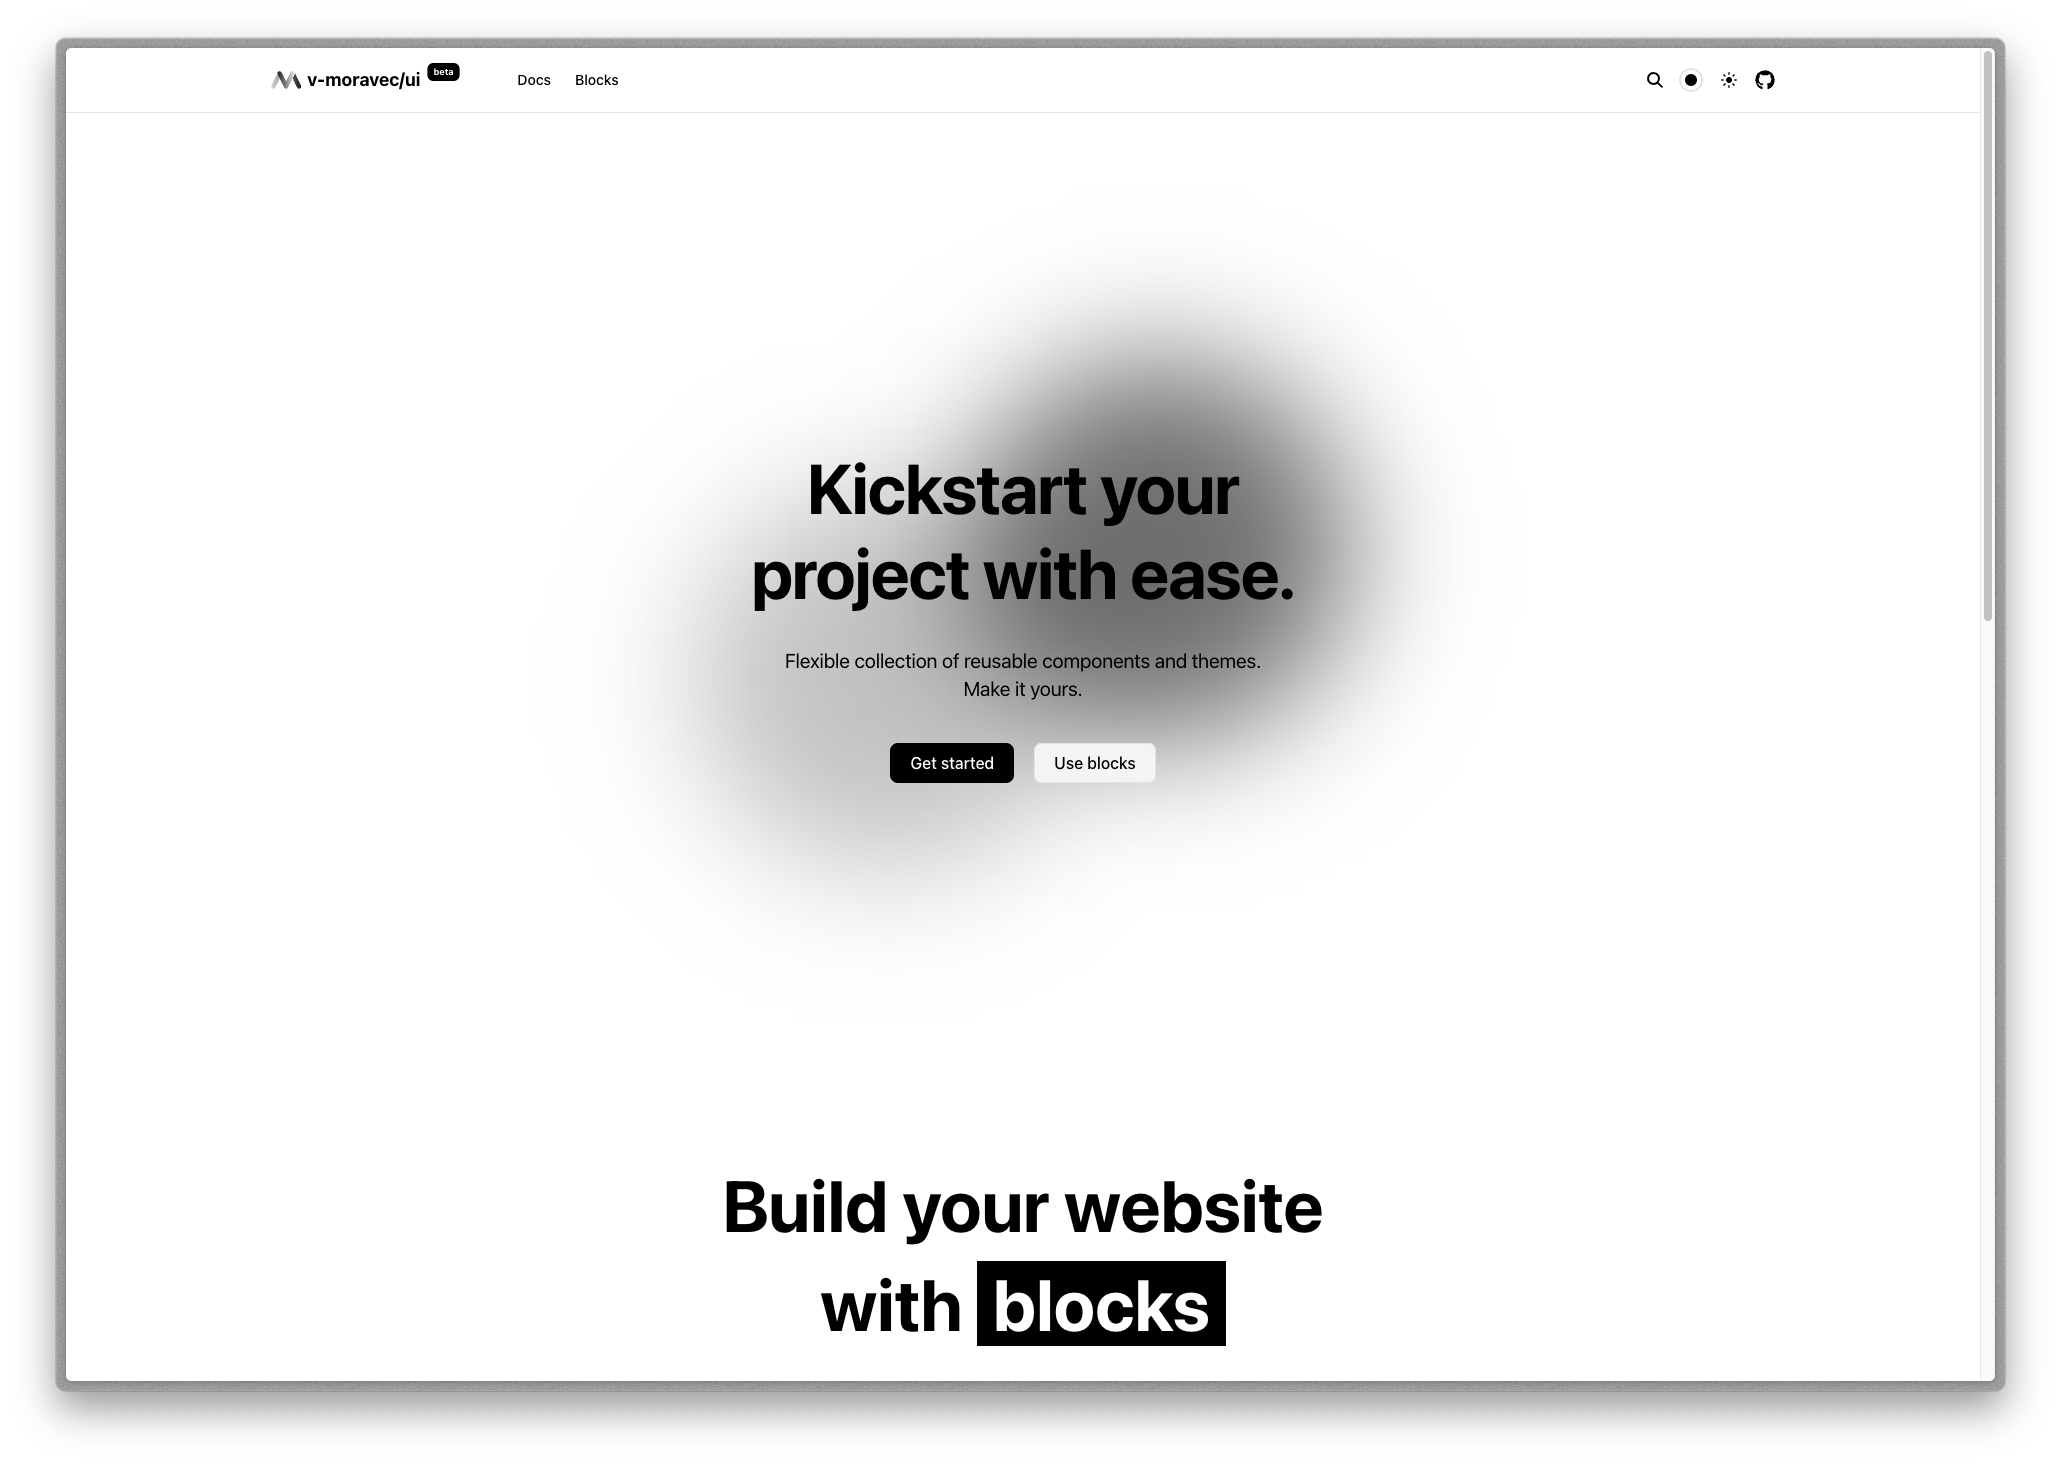
\includegraphics[width=\textwidth]{images/landing-page}
  \caption{Úvodní obrazovka} \label{picture:documentation:landing-page}
\end{figure}

\begin{figure}[h]
  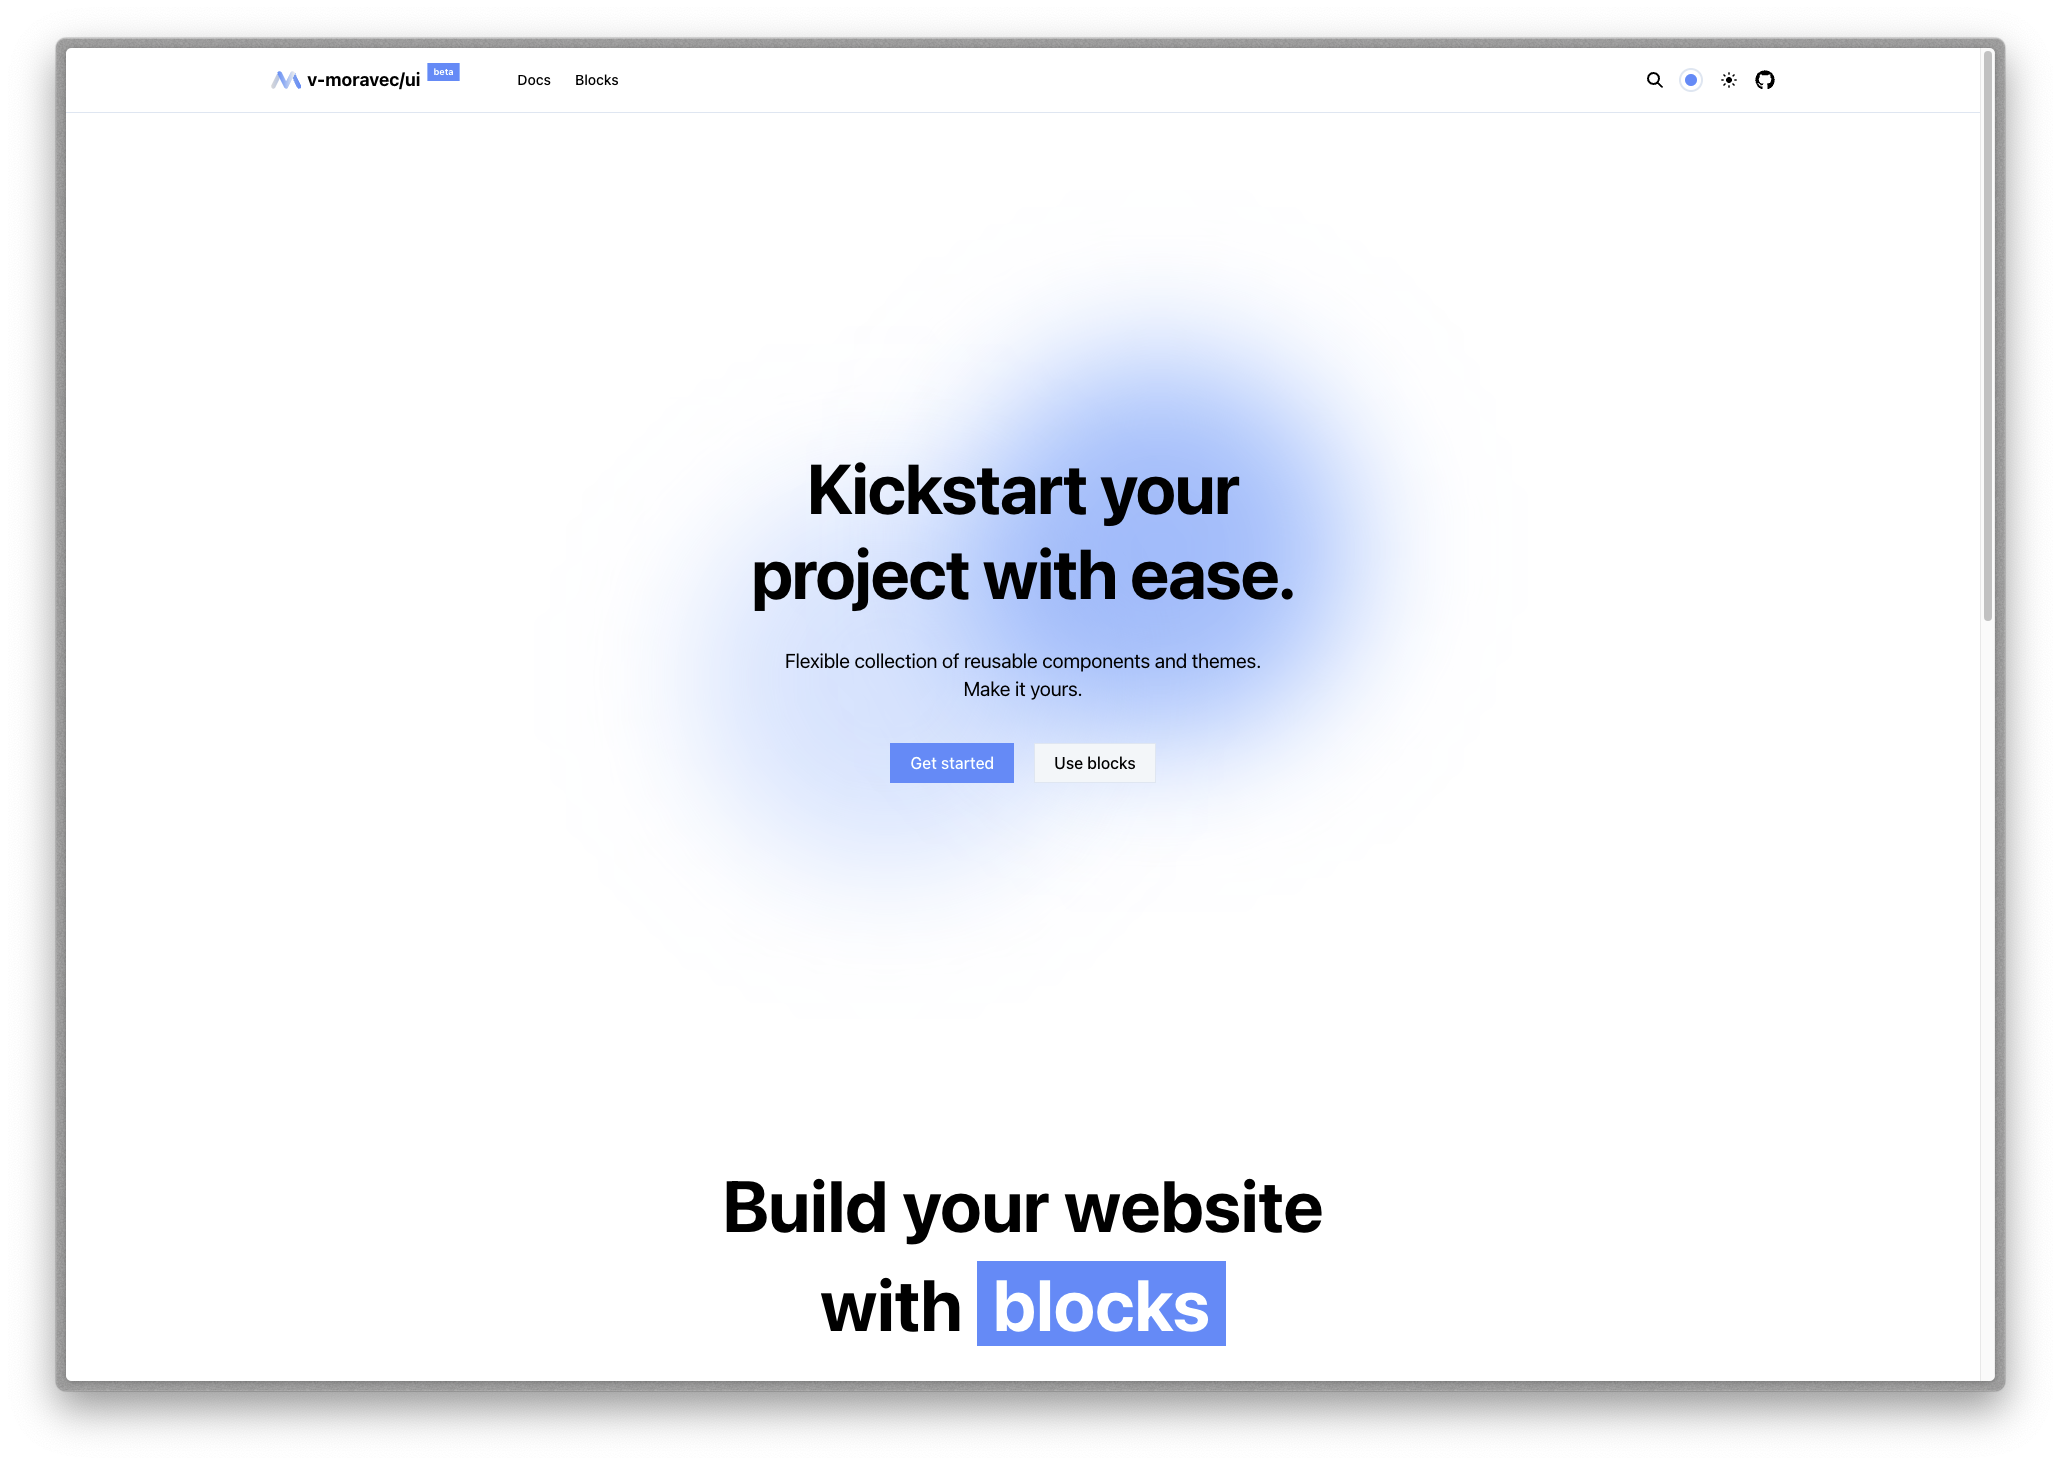
\includegraphics[width=\textwidth]{images/landing-page-blue}
  \caption{Úvodní obrazovka - modrá verze} \label{picture:documentation:landing-page-blue}
\end{figure}

\begin{figure}[h]
  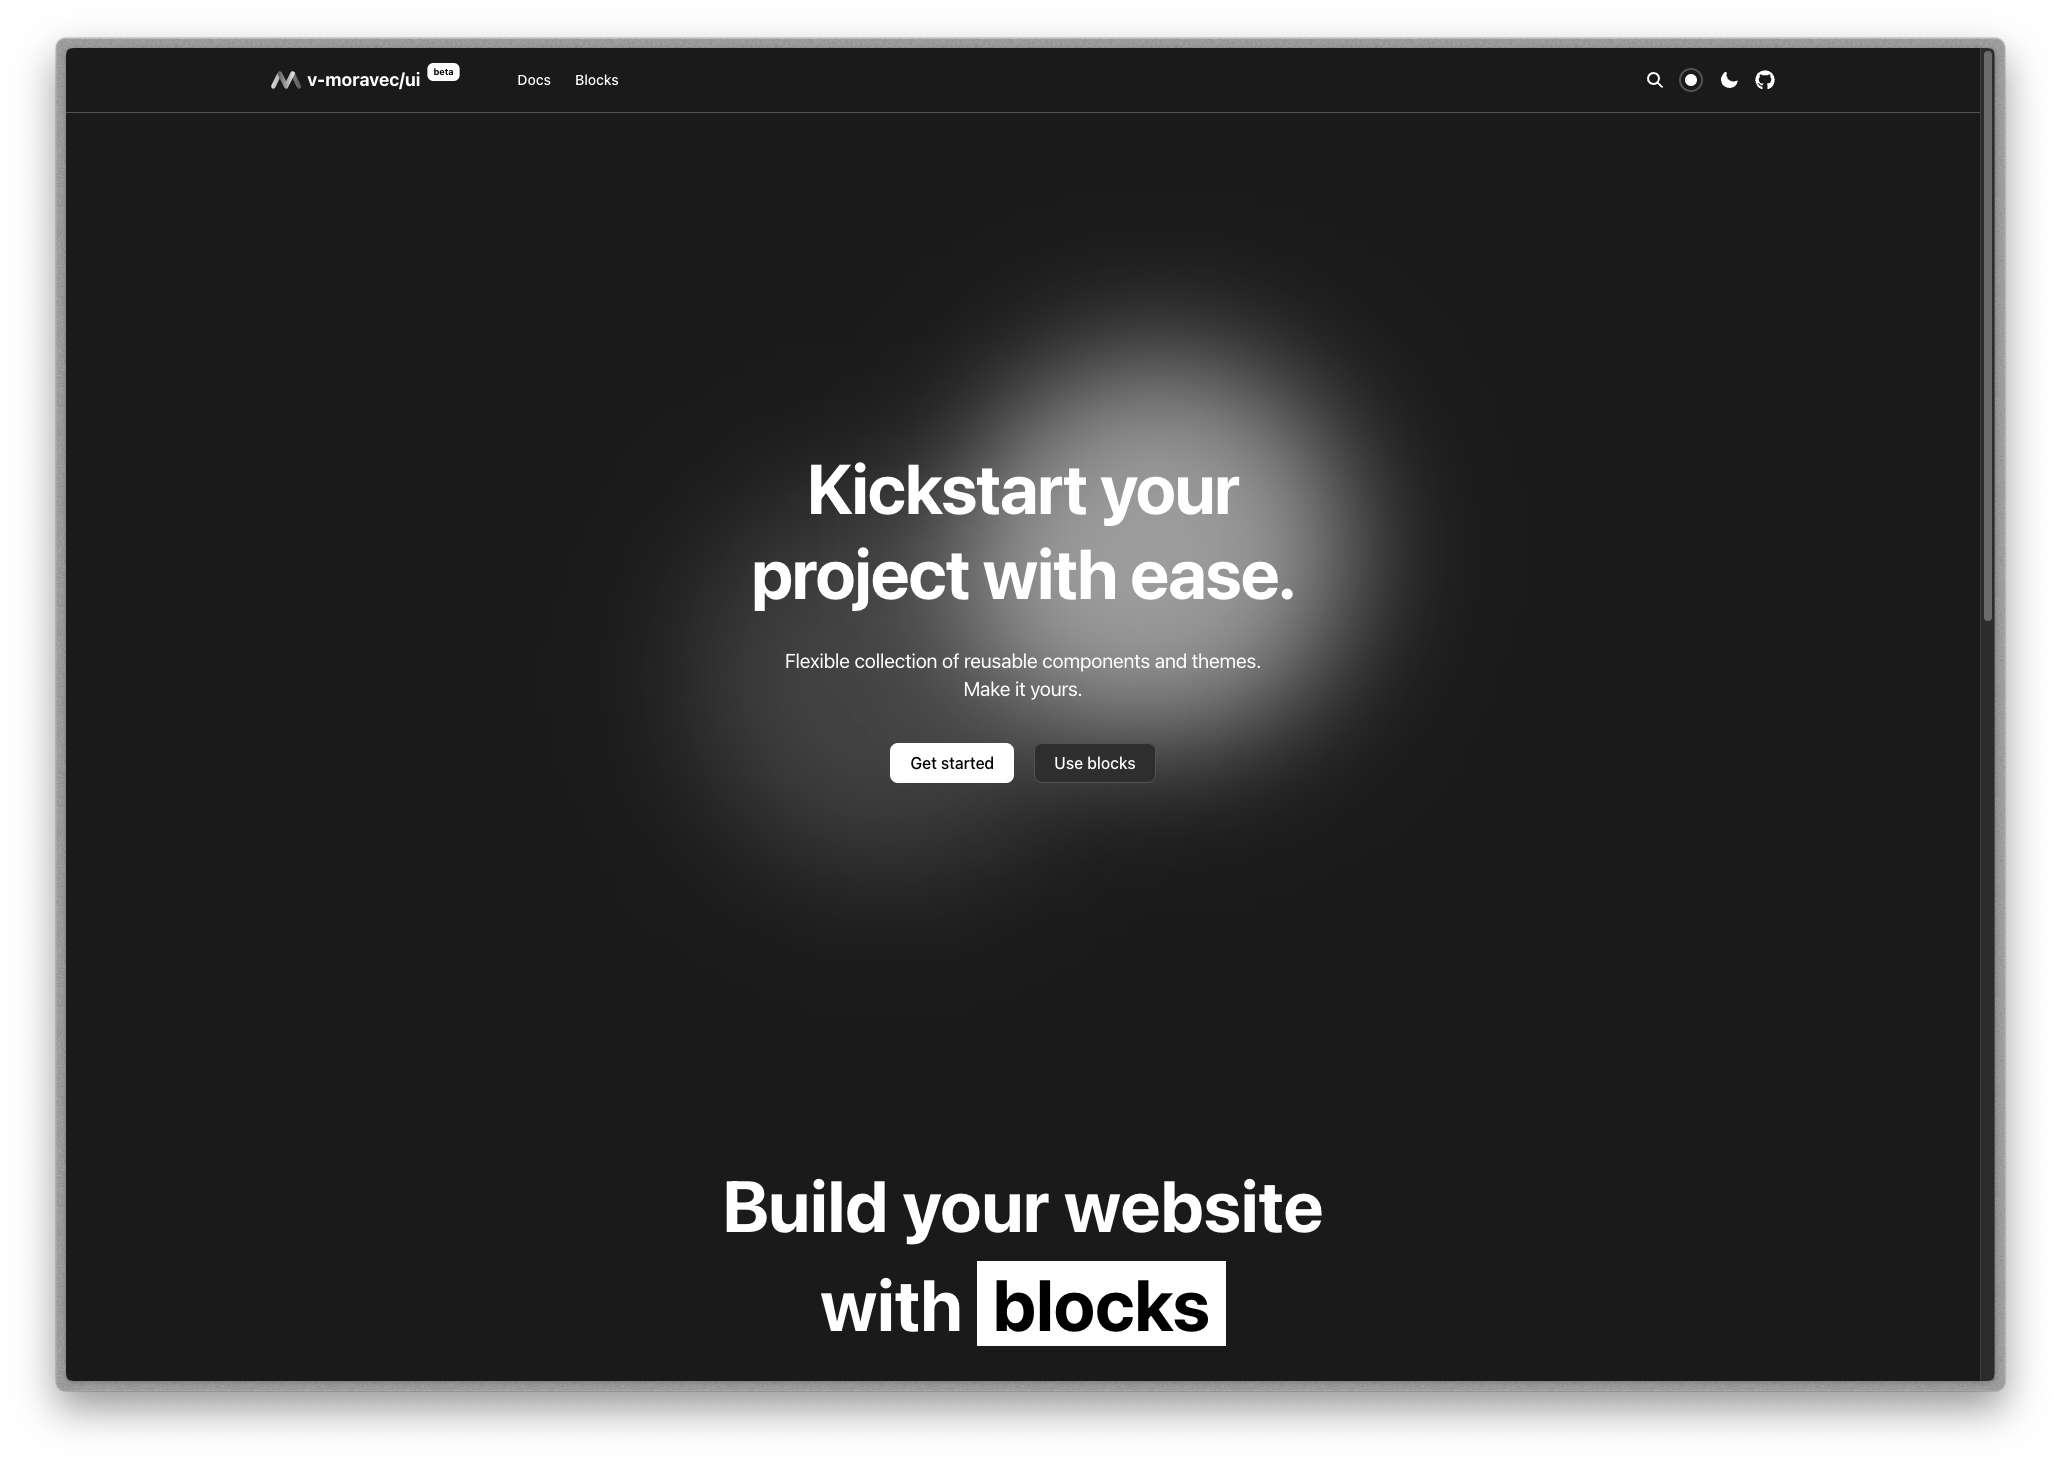
\includegraphics[width=\textwidth]{images/landing-page-dark}
  \caption{Úvodní obrazovka - tmavá verze} \label{picture:documentation:landing-page-dark}
\end{figure}

\begin{figure}[h]
  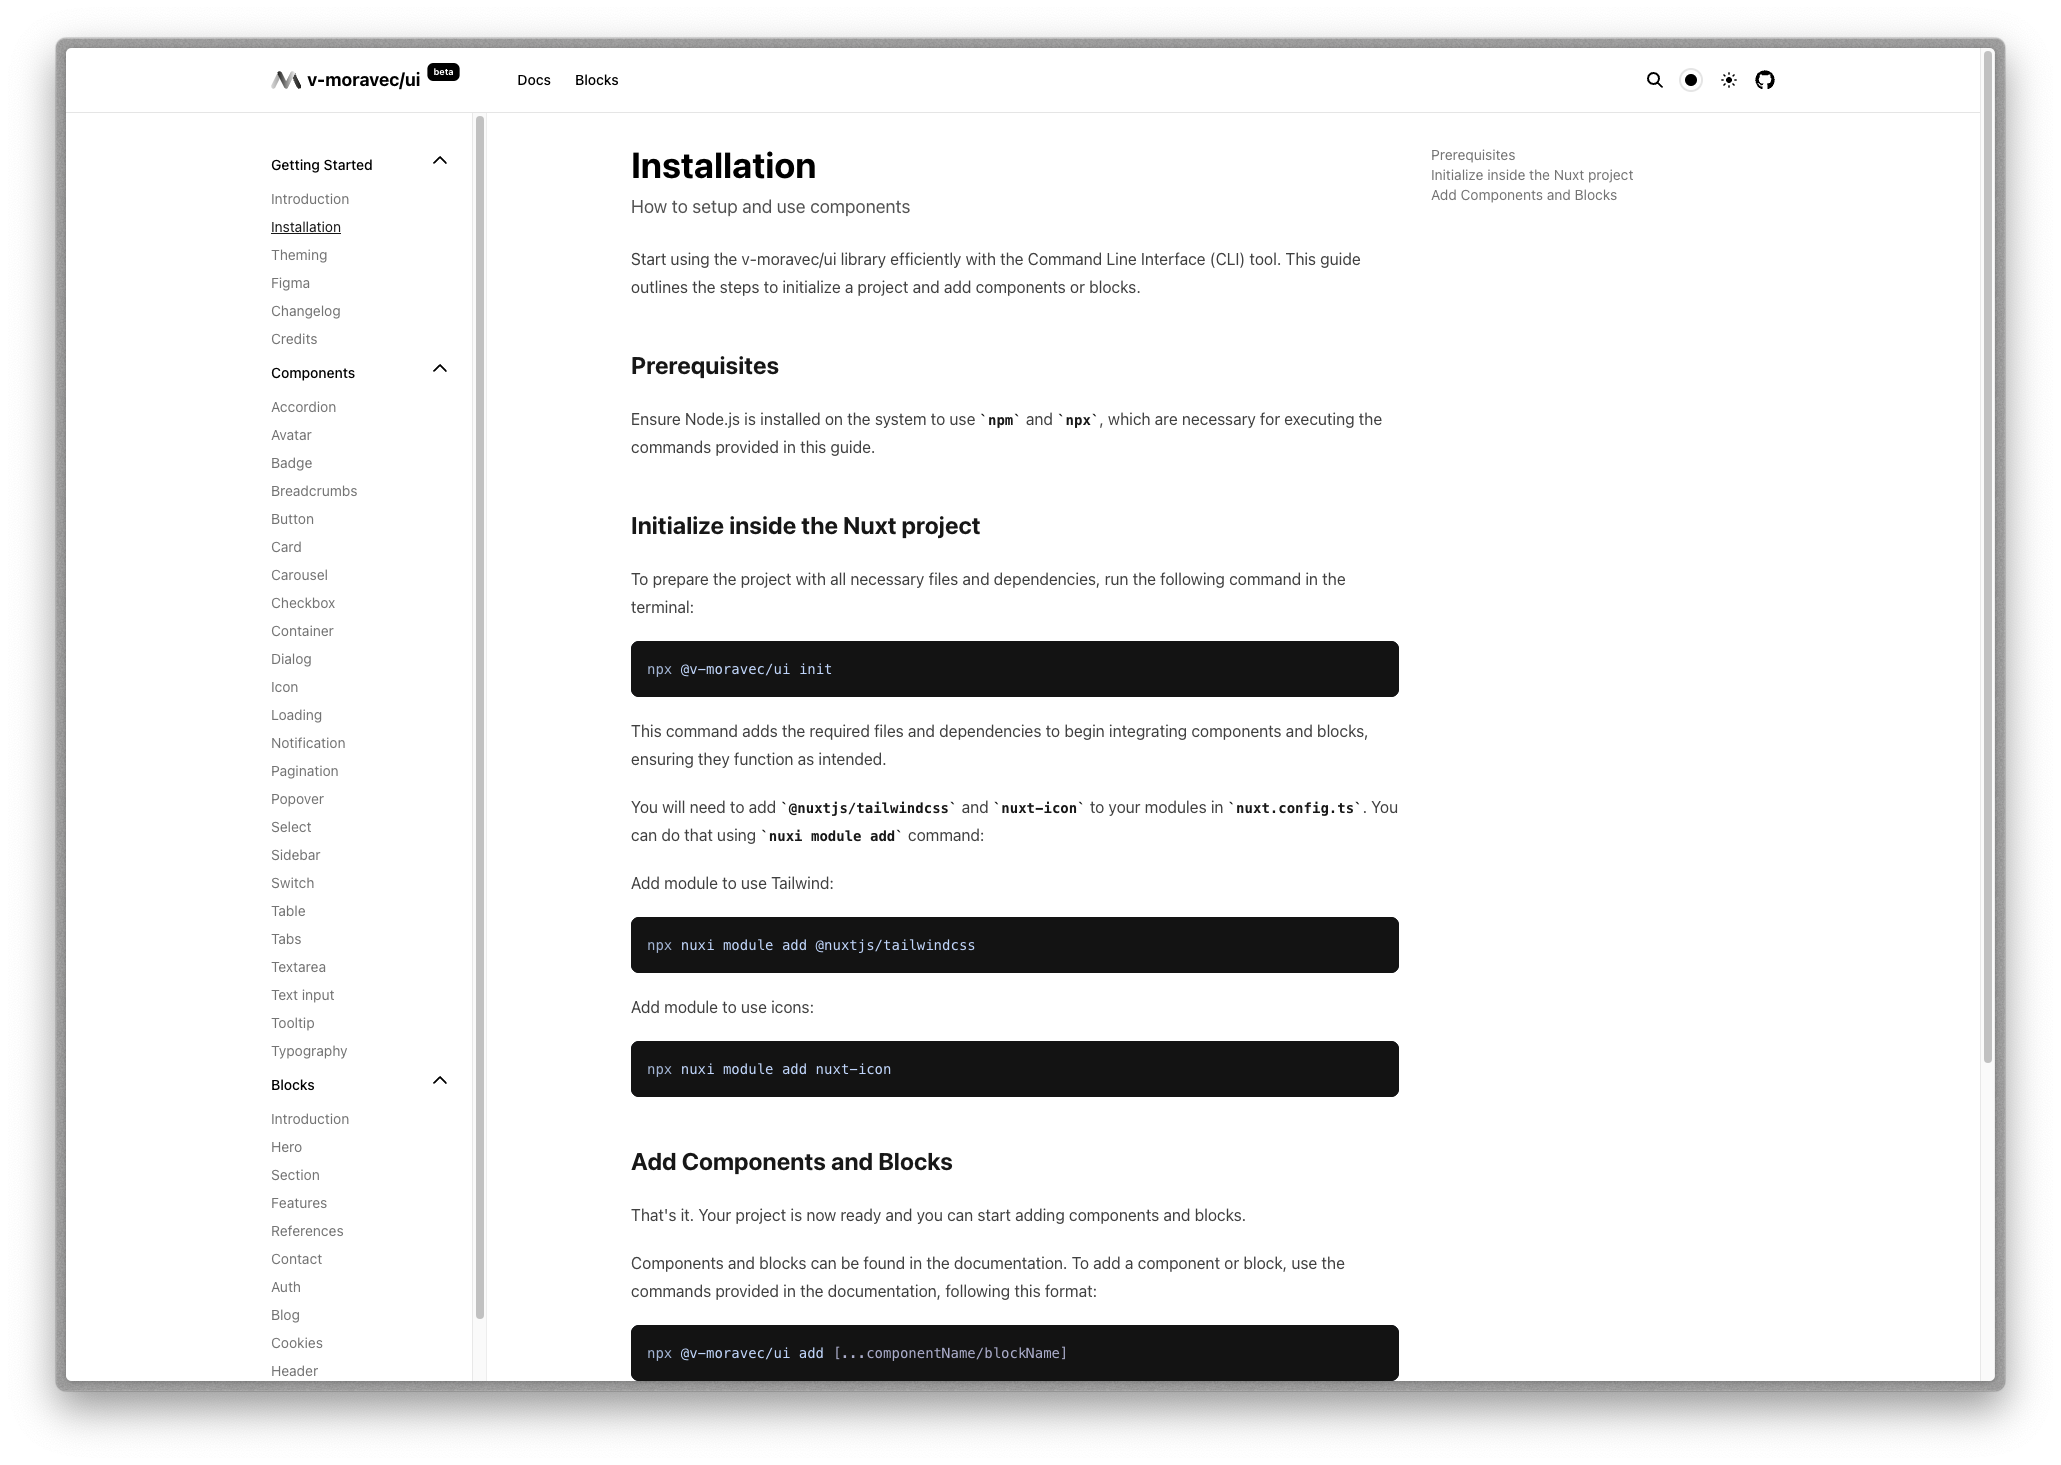
\includegraphics[width=\textwidth]{images/installation}
  \caption{Instalace} \label{picture:documentation:installation}
\end{figure}

\begin{figure}[h]
  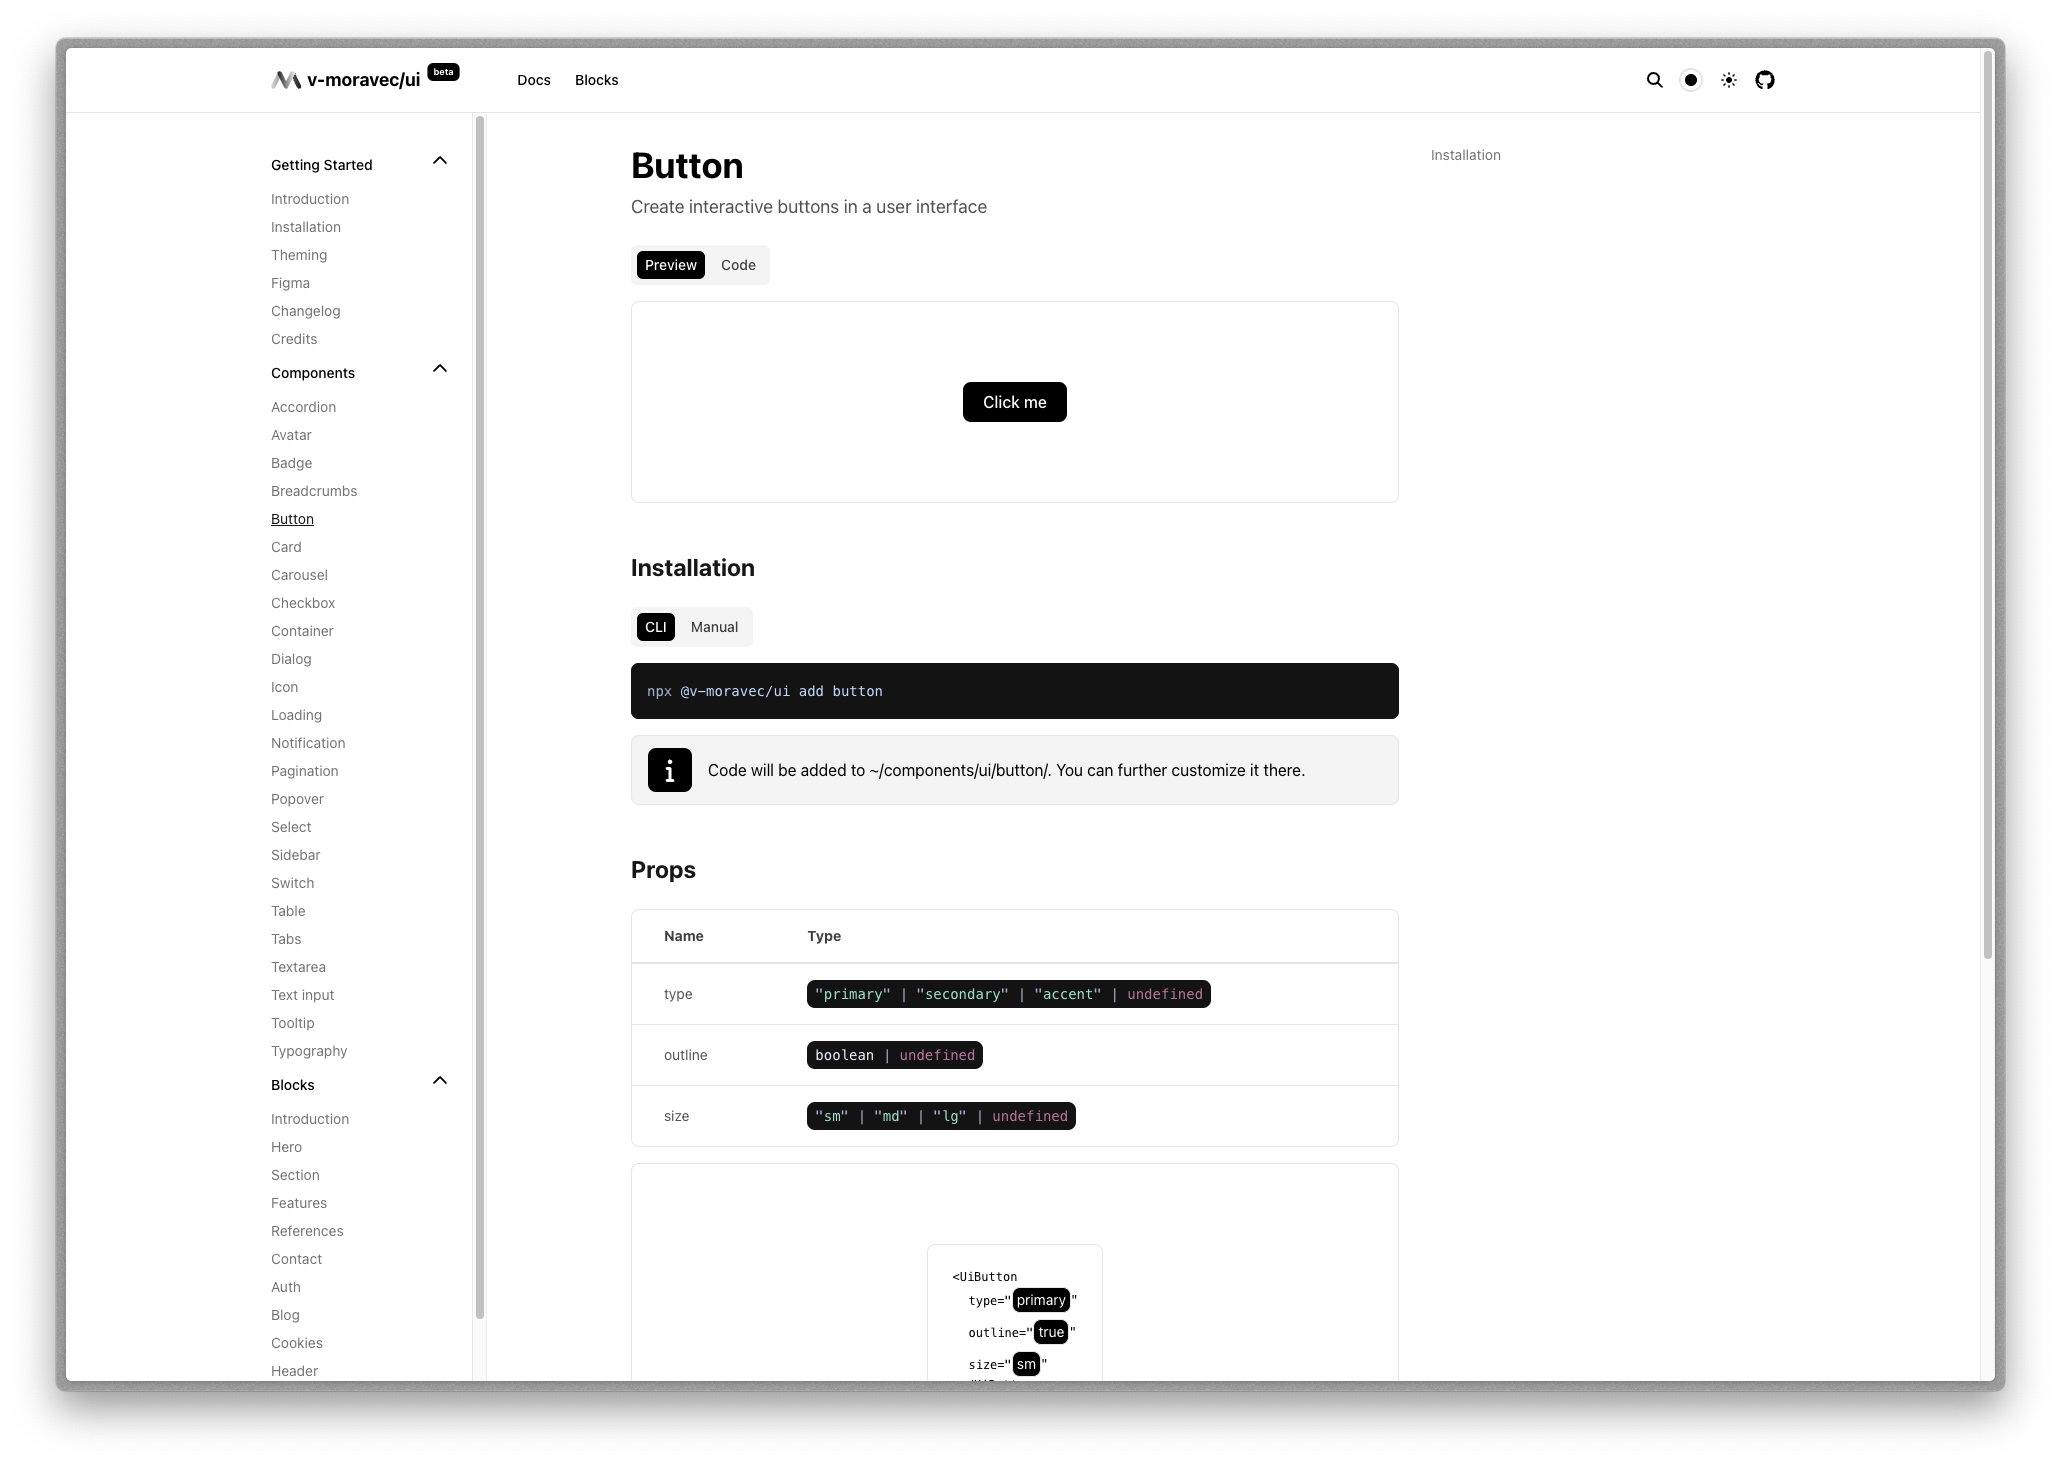
\includegraphics[width=\textwidth]{images/component-preview}
  \caption{Zobrazení komponenty} \label{picture:documentation:component-preview}
\end{figure}

\begin{figure}[h]
  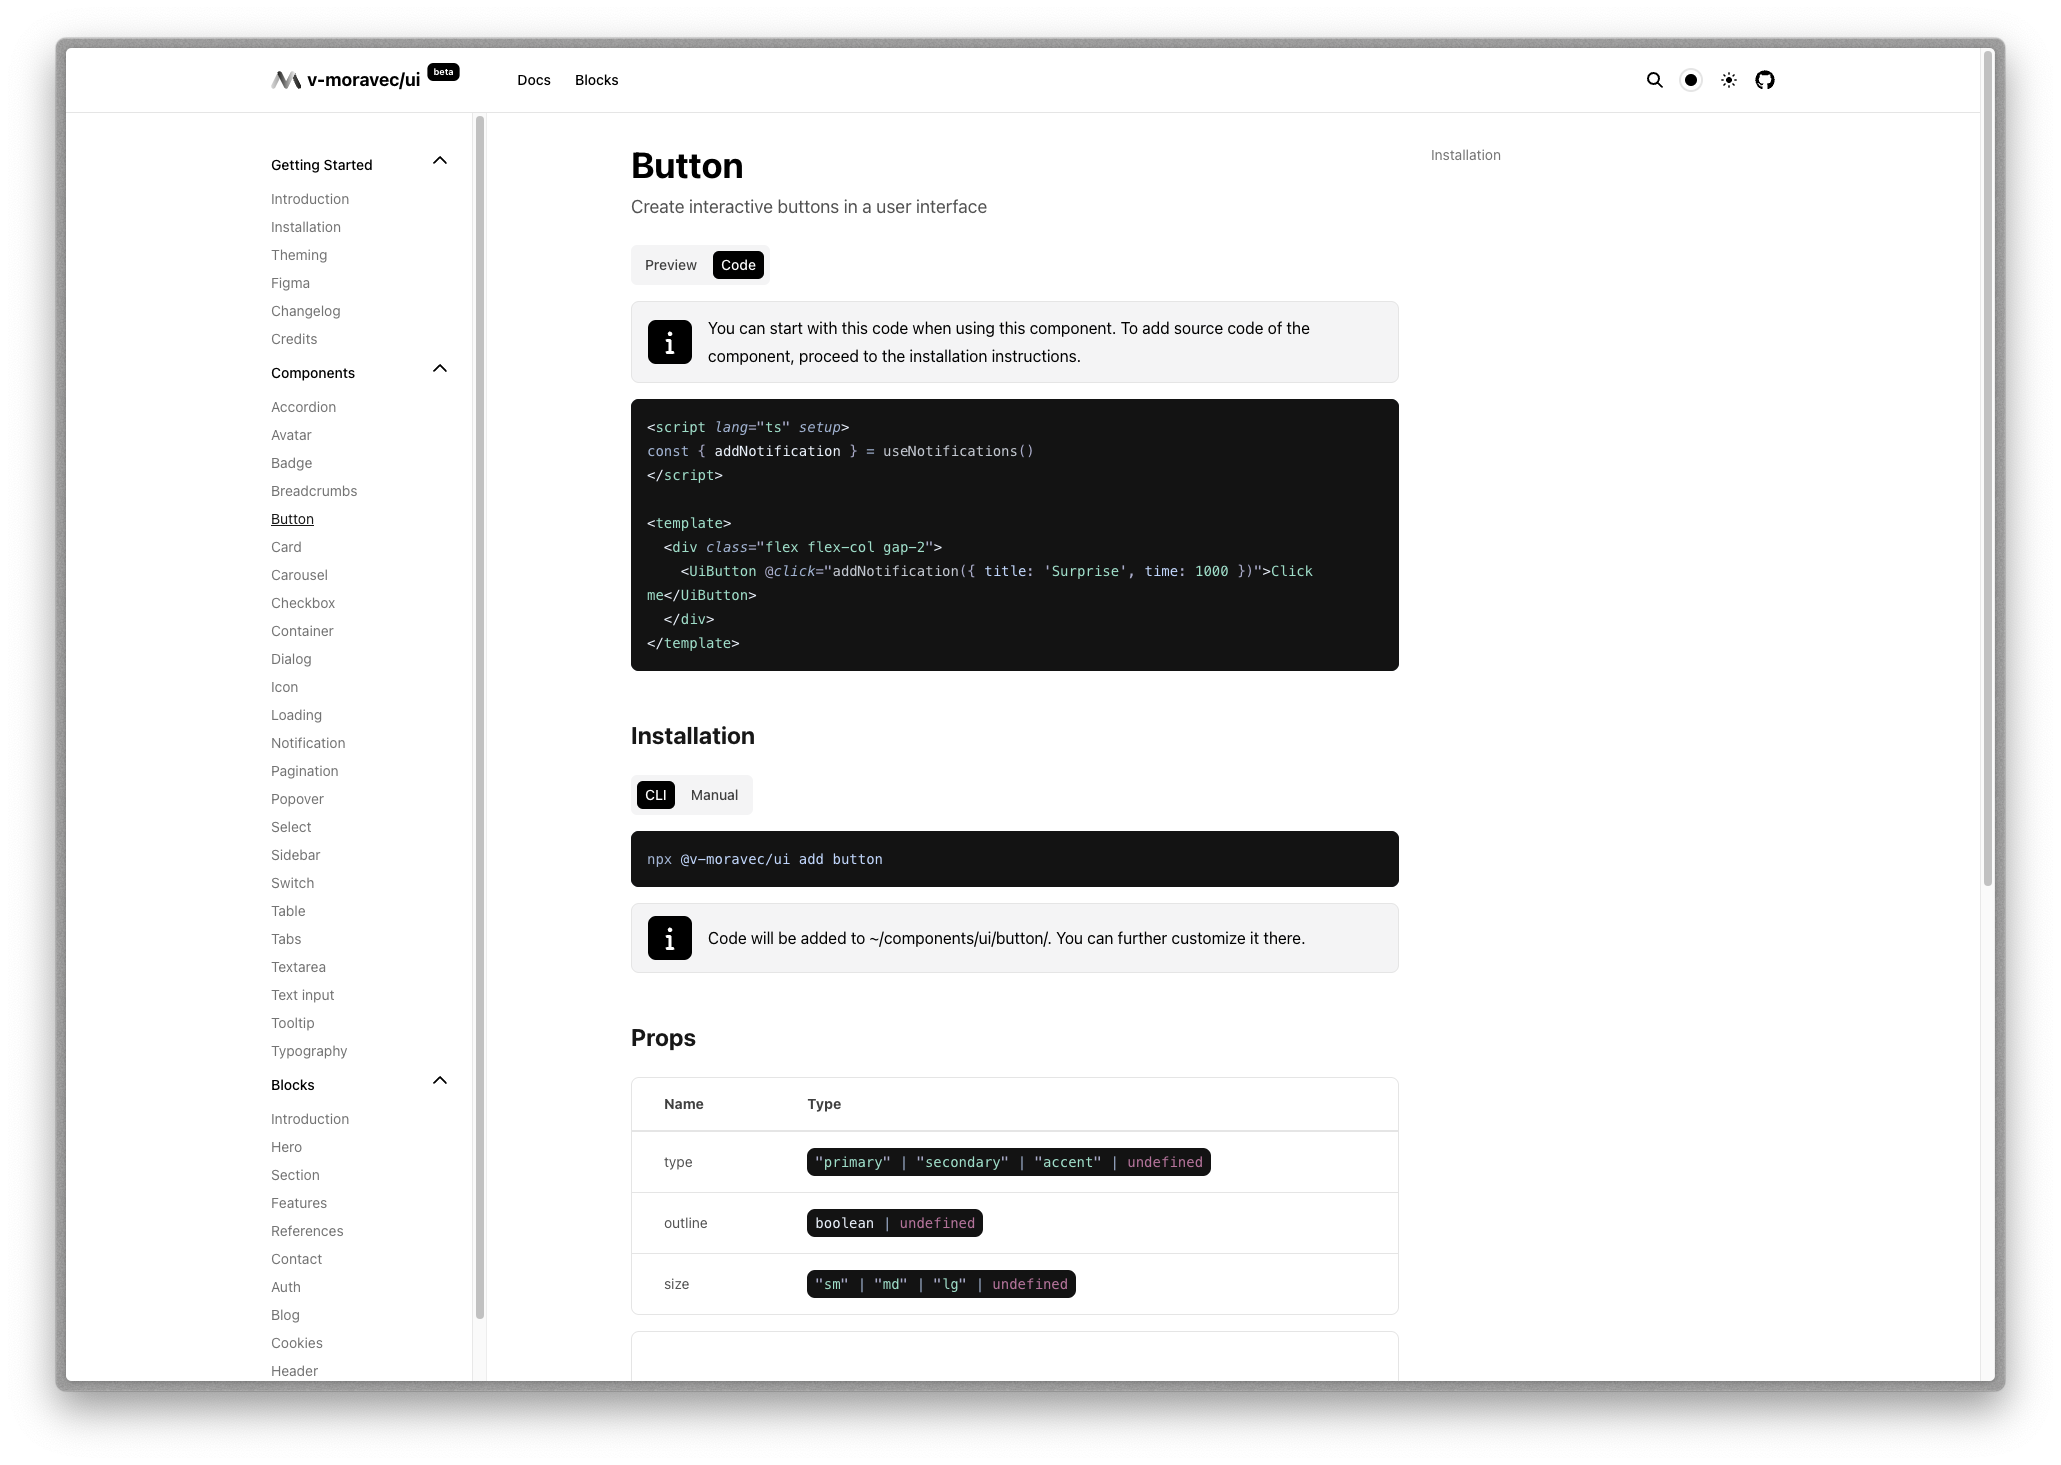
\includegraphics[width=\textwidth]{images/component-code}
  \caption{Kód komponenty} \label{picture:documentation:component-code}
\end{figure}

\begin{figure}[h]
  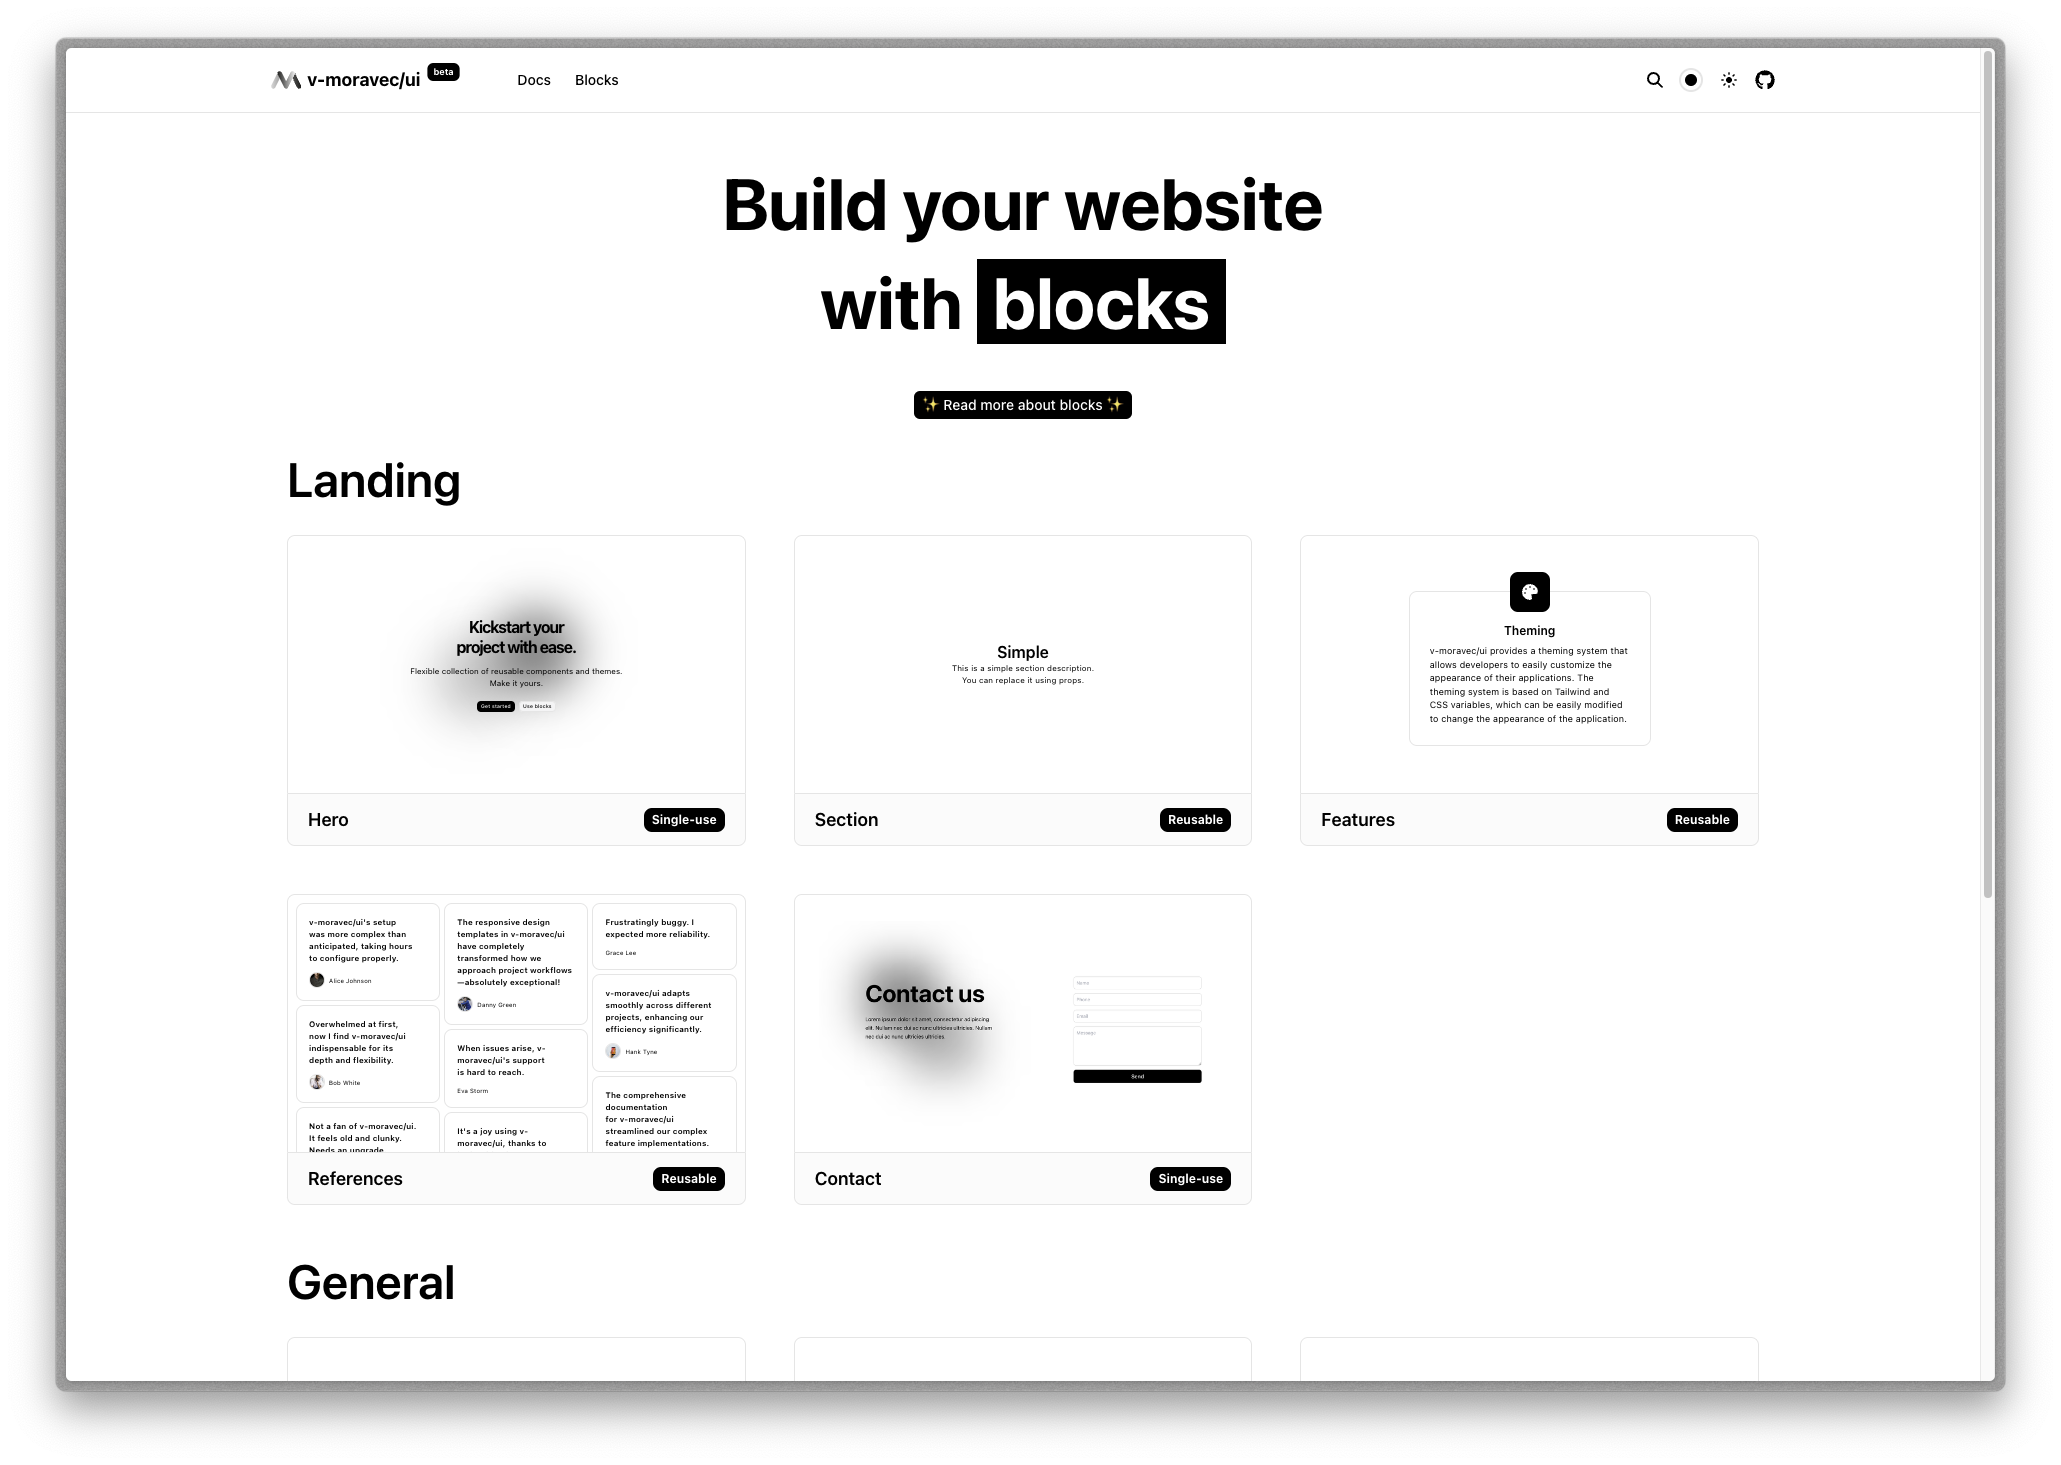
\includegraphics[width=\textwidth]{images/blocks}
  \caption{Seznam bloků} \label{picture:documentation:blocks}
\end{figure}

\begin{figure}[h]
  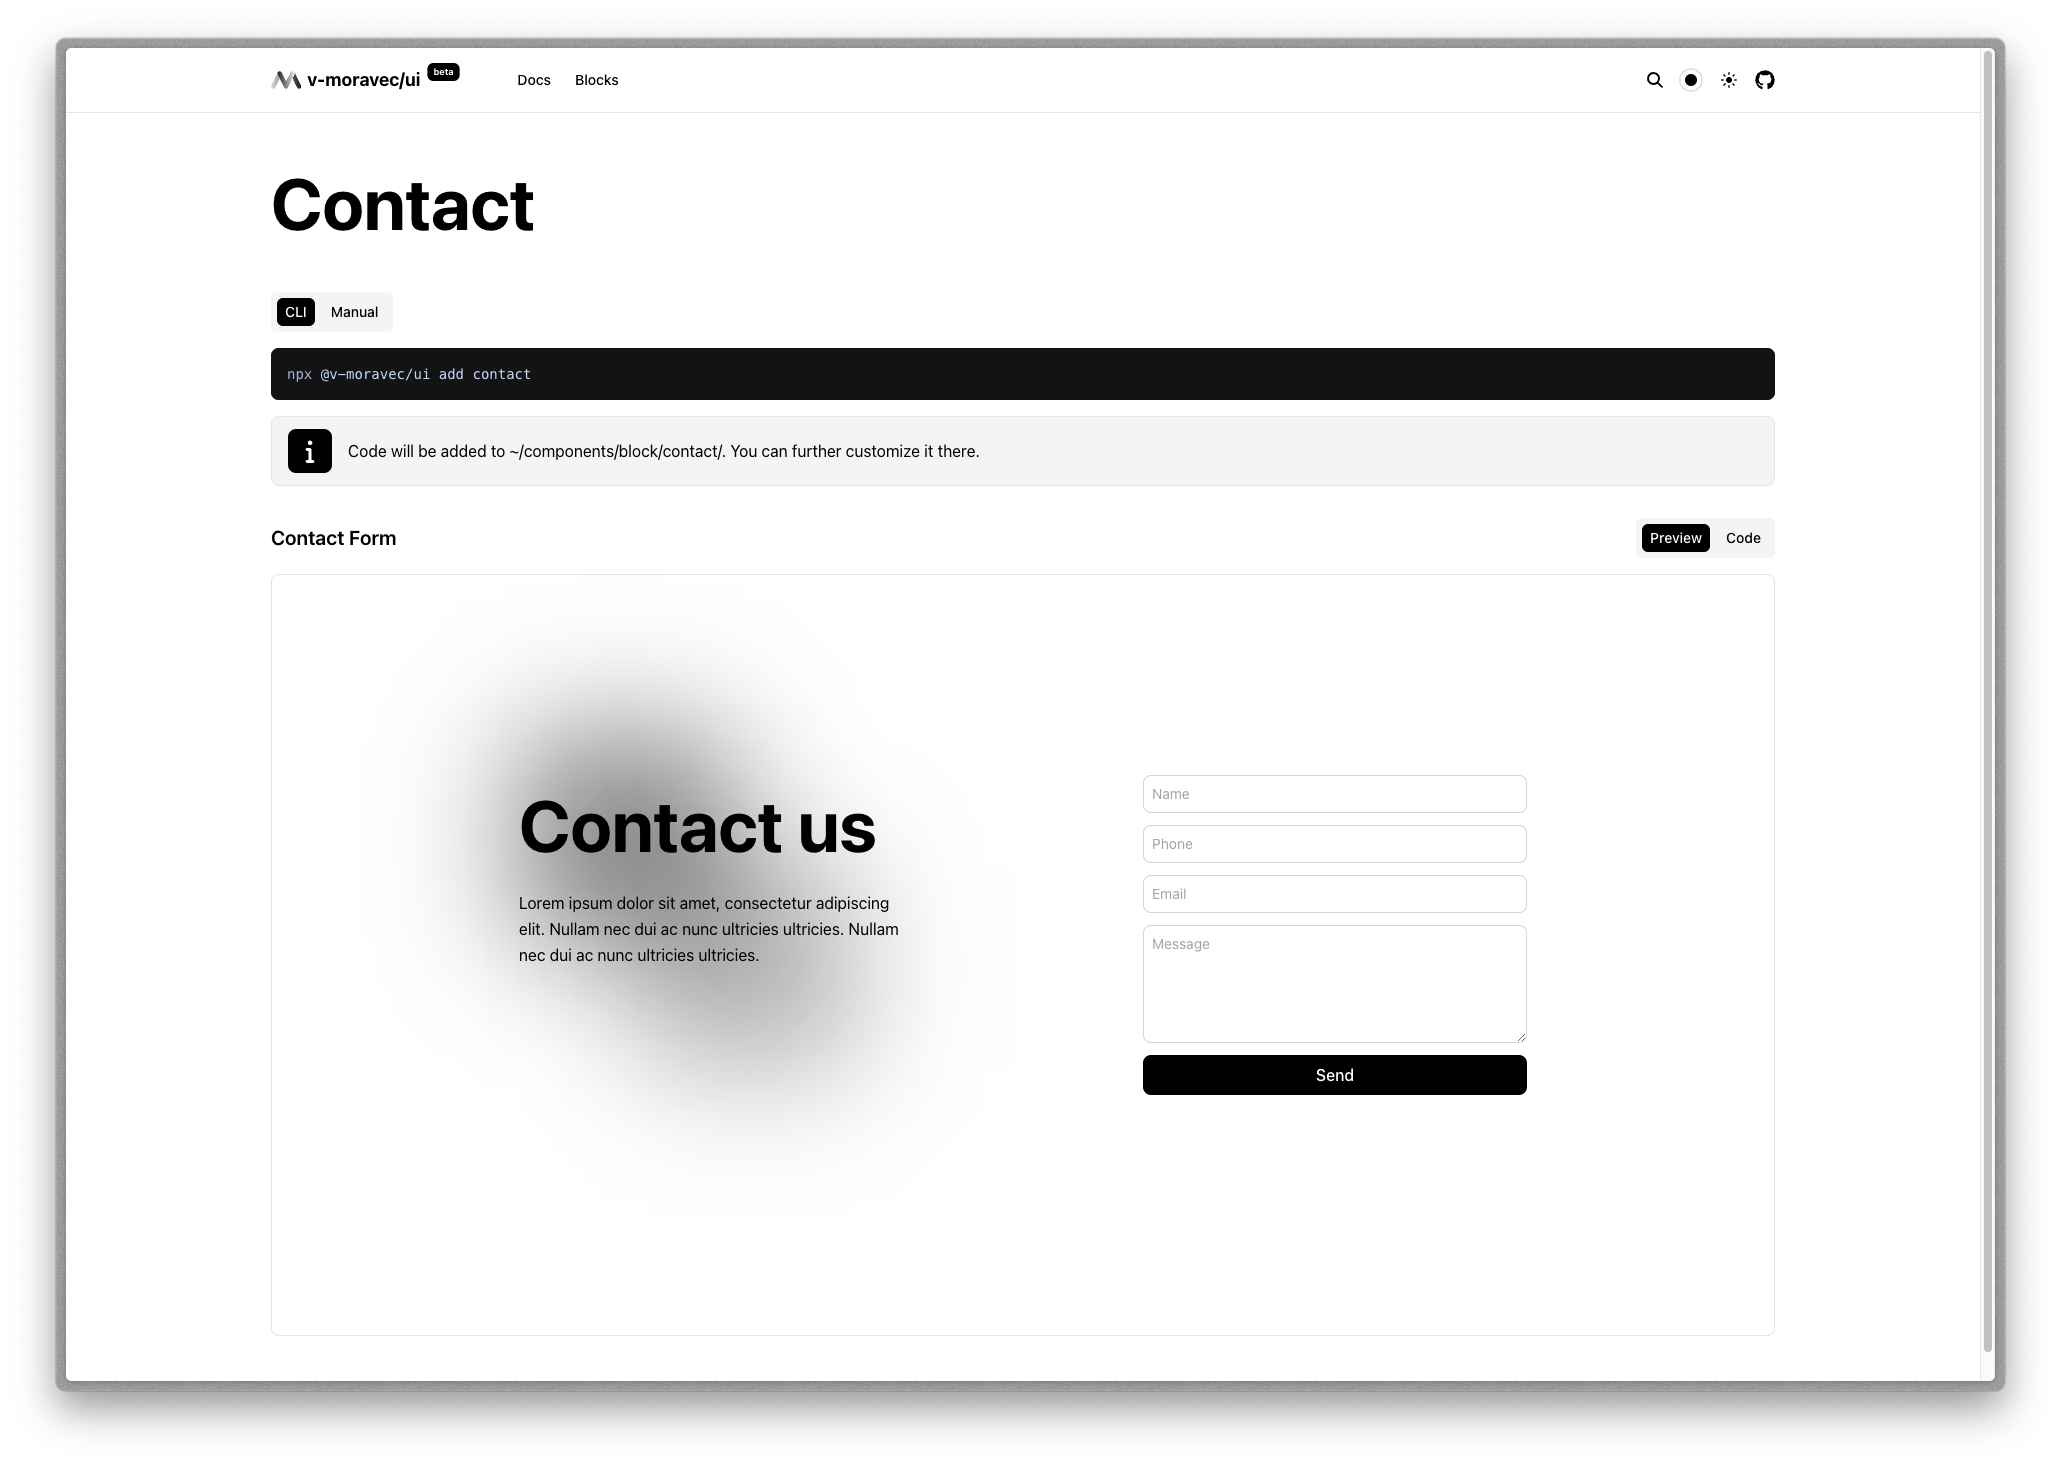
\includegraphics[width=\textwidth]{images/block-contact-docs}
  \caption{Blok kontaktní formulář} \label{picture:documentation:block-contact-docs}
\end{figure}

\chapter{Ukázky kódu}

\begin{listing}[h]
  \caption{Vytvoření endpointu pro získání kódu komponent}
  \label{lst:link-to-endpoint}
  \begin{code}
nuxt.hook('nitro:config', (nitroConfig) => {
nitroConfig.virtual = nitroConfig.virtual || {}
  nitroConfig.virtual['#component-list/nitro'] = () =>
      readFileSync(join(nuxt.options.buildDir, '/component-list.mjs'), 'utf-8')
})

addServerHandler({
  method: 'get',
  route: '/api/component-list/:component?',
  handler: resolver.resolve('../server/api/component-list.get'),
})
\end{code}
\end{listing}

\begin{listing}[h]
  \caption{Endpoint pro získání kódu komponent}
  \label{lst:code-example-endpoint}
  \begin{code}
import { defineEventHandler, createError, appendHeader } from 'h3'
import { pascalCase } from 'scule'
// @ts-expect-error
import components from '#code-examples/nitro'

export default defineEventHandler((event) => {
  appendHeader(event, 'Access-Control-Allow-Origin', '*')
  const componentName = (event.context.params['component?'] || '').replace(/\.json$/, '')
  if (componentName) {
    const component = components[pascalCase(componentName)]
    if (!component) {
      throw createError({
        statusMessage: 'Examples not found!',
        statusCode: 404,
      })
    }
    return component
  }
})  
\end{code}
\end{listing}

\begin{listing}[h]
  \caption{Transformace dat komponent a bloků pro využití v rámci CLI}
  \label{lst:cli-data-transform}
  \begin{code}
const code = await fsp.readFile(component.shortPath, 'utf-8')

const script = code.match(/<script[^]*?<\/script>/ms)?.[0]
const template = code.match(/<template[^]*?<\/template>/ms)?.[0]

const dependencies = script
  ? removeDuplicates(
      script
      .match(/import[^]*?from[^]*?['"]([^'"]+)['"]/gm)
      ?.map((dependency) => {
          return dependency.split('from')[1].trim().replace(/['";]/g, '')
      })
      .filter((v) => !v.startsWith('.') && !v.startsWith('~') && v !== 'vue' && v !== 'nuxt')
  )
  : undefined

const composableDependencies = script
  ? removeDuplicates(
      script
      .match(/use[a-zA-z]*?\(/gm)
      ?.map((dependency) => {
          return dependency.trim().replace(/['"();]/g, '')
      })
      .filter((v) => !v.startsWith('.') && !v.startsWith('~') && v !== 'vue' && v !== 'nuxt')
  )
  : undefined

const uiDependencies = template
  ? removeDuplicates(
      template.match(/<Ui[^>]+>/gm)?.map((v) =>
      v
          .slice(1, -1)
          .split(' ')[0]
          .trim()
          .split(/(?=[A-Z])/)[1]
          .toLowerCase()
      )
  )
  : undefined

components[component.pascalName] = {
  code,
  uiDependencies,
  dependencies,
  composableDependencies,
  shortPath: component.shortPath,
  pascalName: component.pascalName,
}
\end{code}
\end{listing}

\begin{listing}[h]
  \caption{Komponenta pro zvýraznění kódu}
  \label{lst:code-highlighter}
  \begin{code}[html]
<script lang="ts" setup>
import { transformContent } from '@nuxt/content/transformers'

const props = defineProps<{
  name: string
  class?: string
}>()

const data = await fetchCodeExample(props.name)

const hasCode = computed(() => data?.code)

const highlighter = await loadShiki()
const { data: ast } = await useAsyncData(`content-example-${props.name}-ast`, () =>
  transformContent('content:_markdown.md', `\`\`\`vue\n${data?.code ?? ''}\n\`\`\``, {
    markdown: {
      highlight: {
        highlighter,
        theme: {
          light: 'poimandres',
          default: 'poimandres',
          dark: 'poimandres',
        },
      },
    },
  })
)
</script>

<template>
  <div class="my-4" v-if="hasCode">
    <ContentRenderer :value="ast" class="[&>div>pre]:!mt-0 [&>div>pre]:overflow-auto [&>div>pre]:!rounded-t-none" />
  </div>
</template>
\end{code}
\end{listing}
 % include `appendix.tex' from `text/' subdirectory

\backmatter % do not remove this command

\printbibliography[title = {Zdroje}] % print out the BibLaTeX-generated bibliography list

\chapter{Obsah přiloženého média}

	\dirtree{%
		.1 README.md\DTcomment{stručný popis obsahu média}.
		.1 master-thesis\DTcomment{zdrojová forma práce ve formátu \LaTeX{}}.
		.1 DP\_Moravec\_Vojtech\_2024.pdf\DTcomment{text práce ve formátu PDF}.
		.1 CodingLab.xd\DTcomment{grafické návrhy v aplikaci Adobe XD}.
	}
 % include `medium.tex' from `text/' subdirectory

\end{document}
